\documentclass[
  11pt,
  open=any,           % Replaces 'openany'
  bibliography=totoc, % Adds Bibliography to TOC
  numbers=noenddot    % Removes trailing dots in headings (e.g., 1.1)
]{scrbook}

% Standard AMS math & theorem setup
\usepackage{amsmath}
\usepackage{amssymb}
\usepackage{amsthm}
\usepackage{bm}

% Force each \section to start on a new page
\AddToHook{cmd/section/before}{\clearpage}

\usepackage[numbers,sort&compress]{natbib}

\usepackage{graphicx}
\graphicspath{{figures/}} % Searches the figures/ subfolder automatically
\usepackage{esint}
\usepackage{xcolor}
\usepackage{multirow}
\usepackage{setspace}
\usepackage{framed}
\usepackage[english]{babel}
\usepackage{wrapfig}
\usepackage{epigraph}
\usepackage{enumitem}

\usepackage[margin=2.6cm]{geometry}
\usepackage{hyperref}
\usepackage{microtype}



% AMS theorem styles integrated into scrbook
\theoremstyle{plain}
\newtheorem{thm}{Theorem}[chapter]
\newtheorem{lem}[thm]{Lemma}
\newtheorem{pos}[thm]{Postulate}

% --- Custom Macros ---
%\newcommand{\bs}[1]{\symbf{#1}}

\newcommand{\ie}{{\emph{i.e.~}}}
\makeatletter
\newcommand{\rmnum}[1]{\romannumeral #1}
\newcommand{\Rmnum}[1]{\expandafter\@slowromancap\romannumeral #1@}
\makeatother
\newcommand{\alert}[1]{{\color{red}{#1}}}
\newcommand{\eg}{{\emph{e.g.~}}}
\newcommand{\etc}{{\emph{etc.~}}}

\newcommand{\p}[1]{{#1}^\prime}

\newcommand{\imth}{\hspace{1pt}\mathrm{i}\hspace{1pt}}
\newcommand{\mbz}{{\mathbb{Z}}}
\newcommand{\id}{\mathbb{I}}
\newcommand{\ce}{\mathcal{E}}
\newcommand{\ch}{\mathcal{H}}
\newcommand{\ct}{{\mathcal{T}}}
\newcommand{\fp}{{\symbf{P}_f}}

\newcommand{\sx}{\sigma_x}
\newcommand{\sy}{\sigma_y}
\newcommand{\sz}{\sigma_z}
\newcommand{\plash}[1]{#1\!\!\!/}

\newcommand{\bct}{\begin{center}}
\newcommand{\ect}{\end{center}}
\newcommand{\bpm}{\begin{pmatrix}}
\newcommand{\epm}{\end{pmatrix}}
\newcommand{\bal}{\begin{align}}
\newcommand{\eal}{\end{align}}
\newcommand{\bfr}{\begin{framed}}
\newcommand{\efr}{\end{framed}}
\newcommand{\re}{\operatorname{Re}}
\newcommand{\im}{\operatorname{Im}}
\newcommand{\dif}[1]{\mathrm{d}{#1}}

\newcommand{\dket}[1]{|{#1}\rangle}
\newcommand{\dbra}[1]{\langle{#1}|}
\newcommand{\expval}[1]{\langle{#1}\rangle}
\newcommand{\ketbra}[2]{\lvert #1\rangle\!\langle #2\rvert}
\newcommand{\proj}[1]{|#1\rangle\langle#1|}
\newcommand{\trace}{\operatorname{Tr}}

\newcommand{\arxiv}[1]{\href{http://arxiv.org/abs/#1}{#1}}


\newcommand{\sumr}{\sum_{\symbf{r}}}
\newcommand{\sumk}{\sum_{\symbf{k}}}
\newcommand{\referto}[1]{\begin{itemize}\item Refer to {#1}\end{itemize}}


\linespread{1}

% Section numbering depth
\setcounter{tocdepth}{2}
\setcounter{secnumdepth}{3}

% Hanging indents for publications
\def\rrr#1\\{\par
\medskip\hbox{\vbox{\parindent=2em\hsize=6.12in
\hangindent=4em\hangafter=1#1}}}

\def\CourseNo{7501}
\def\CourseTitle{Quantum Mechanics 1 (graduate core course)}
\def\Semester{Autumn 2026}
\def\Jobs{Professor}

\title{Physics \CourseNo\ (\Semester)\\ \CourseTitle}
\author{Yuan-Ming Lu}
\date{\today}

\begin{document}

\frontmatter

\begin{center}
{\LARGE Physics \CourseNo\ (\Semester)\par}
\vspace{0.5em}
{\LARGE \CourseTitle\par}
\vspace{1.5em}
{\large Yuan-Ming Lu\par}
\vspace{1em}
{\large \today\par}
\end{center}

\bigskip
\noindent\textbf{Abstract.} In this elementary course of quantum mechanics, we will learn the mathematical basis of quantum mechanics (i.e. linear algebra), the postulates of quantum theory, and how to use quantum mechanics to understand microscopic quantum phenomena.

\clearpage

\tableofcontents
\clearpage

\mainmatter
\setcounter{chapter}{-1}
\chapter{Course Information}

\minisec{Instructor}
\Jobs~\href{https://physics.osu.edu/people/lu.1435}{\textbf{Yuan-Ming Lu}}

\minisec{Contact Information}
\begin{itemize}
  \item \textbf{Email:} \href{mailto:lu.1435@osu.edu}{lu.1435@osu.edu}
  \item \textbf{Office Phone:} 614-292-3084
  \item \textbf{Office:} 2012 Physics Research Building (PRB)
\end{itemize}

\minisec{Office Hours}
Friday 2:00--3:00\,pm in PRB 2015

\minisec{Lecture Logistics}
\begin{itemize}
  \item \textbf{Location:} \href{https://www.osu.edu/map/building/148}{Scott Lab N050}
  \item \textbf{Time:} Wed. Fri. 11:10\,am -- 12:30\,pm
  \item \textbf{Schedule:} See \href{https://docs.google.com/spreadsheets/d/1czMLda2yYjPPWqLrT6RY-lmh-6S2gPE9/edit?usp=sharing&ouid=110786316698514501494&rtpof=true&sd=true}{Google Spreadsheet}
\end{itemize}

\minisec{Teaching Assistant \& Guided Group Work}
\begin{itemize}
  \item \textbf{Graduate Teaching Assistant (GTA):} Mr. Hyungjun Jeon (\href{mailto:jeon.258@osu.edu}{jeon.258@osu.edu})
  \item \textbf{GTA Office Hours:} Thursday 3:00--4:00\,pm in PRB 2015
  \item \textbf{Guided Group Work (GGW) Sessions:} Thursdays 9:30\,am -- 11:00\,am in PRB 0118. For questions regarding GGW sessions, please contact Dr. Beatriz E Burrola Gabilondo (\href{mailto:burrolagabilondo.1@osu.edu}{burrolagabilondo.1@osu.edu}).
\end{itemize}

\minisec{Prerequisites}
The course will assume physics and mathematics knowledge at the advanced undergraduate level (e.g., basic quantum mechanics, linear algebra, and differential equations), which we will review as needed.

\minisec{Lecture Notes}
Lecture notes will be uploaded to Carmen as PDF files generated from LaTeX sources at least 4 days before each lecture.

% --- Reference Short Macro Definitions ---
\newcommand{\shankar}{\href{https://link.springer.com/book/10.1007/978-1-4757-0576-8}{Shankar}}
\newcommand{\tongqm}{\href{http://www.damtp.cam.ac.uk/user/tong/quantum.html}{TongQM}}
\newcommand{\tongtopics}{\href{http://www.damtp.cam.ac.uk/user/tong/topicsinqm.html}{TongQMTopics}}
\newcommand{\sakurai}{\href{https://doi.org/10.1017/9781108587280}{S\&N}}
\newcommand{\nielsen}{\href{https://doi.org/10.1017/CBO9780511976667}{N\&C}}
\newcommand{\bebera}{\href{https://doi.org/10.1017/9781108525848}{B\&DD}}
\newcommand{\tong}{\href{https://www.cambridge.org/highereducation/books/quantum-mechanics/944A7CDD78F295264B05977DF3853352#overview}{Tong}}
\newcommand{\landau}{\href{https://power1.pc.uec.ac.jp/~toru/notes/LandauLifshitz-QuantumMechanics.pdf}{L$^2$}}
\newcommand{\weinberg}{\href{https://www.cambridge.org/core/books/lectures-on-quantum-mechanics/F739B9577D2473995024FA5E9ABA9B6C}{Weinberg}}
\newcommand{\anastopolous}{\href{https://www.cambridge.org/highereducation/books/quantum-theory/DCDC1557939E38C176EE7FF9334AB8D0#overview}{Anastopoulos}}
\newcommand{\zee}{\href{https://www.amazon.com/Group-Theory-Nutshell-Physicists-Zee/dp/0691162697}{Zee}}
\newcommand{\tinkham}{\href{https://store.doverpublications.com/products/9780486432472}{Tinkham}}
\newcommand{\dresselhaus}{\href{https://link.springer.com/book/10.1007/978-3-540-32899-5}{Dresselhaus}}
\newcommand{\arovas}{\href{https://courses.physics.ucsd.edu/2016/Spring/physics220/LECTURES/GROUP_THEORY.pdf}{Arovas}}

\minisec{Main Textbooks (Recommended but Not Required)}
\begin{itemize}
  \item \href{https://doi.org/10.1017/9781108587280}{\emph{Modern Quantum Mechanics}} by J.J. Sakurai and Jim Napolitano (3rd Edition, Cambridge University Press, 2020)
  \item \href{https://www.cambridge.org/highereducation/books/quantum-mechanics/944A7CDD78F295264B05977DF3853352#overview}{\emph{Quantum Mechanics} (Vol. 3, Lectures on Theoretical Physics)} by David Tong (Cambridge University Press, 2025). Problem sets available at \href{https://www.damtp.cam.ac.uk/user/tong/books/quantum.html}{https://www.damtp.cam.ac.uk/user/tong/books/quantum.html}.
  \item \href{https://link.springer.com/book/10.1007/978-1-4757-0576-8}{\emph{Principles of Quantum Mechanics}} by \href{https://campuspress.yale.edu/rshankar/}{Ramamurti Shankar} (2nd Edition, Plenum Press, 2011)
  \item \href{https://doi.org/10.1017/CBO9780511976667}{\emph{Quantum Computation and Quantum Information}} by Michael Nielsen and Isaac Chuang (Cambridge University Press, 2011)
\end{itemize}

\minisec{Other References}
\begin{itemize}
  \item \href{http://www.damtp.cam.ac.uk/user/tong/quantum.html}{\emph{Lectures on Quantum Mechanics and on Topics in Quantum Mechanics}}, David Tong, University of Cambridge
  \item \href{https://power1.pc.uec.ac.jp/~toru/notes/LandauLifshitz-QuantumMechanics.pdf}{\emph{Quantum Mechanics: Non-Relativistic Theory}} by Lev Landau and L. Lifshitz (2nd Edition, Pergamon Press)
  \item \href{https://www.cambridge.org/core/books/lectures-on-quantum-mechanics/F739B9577D2473995024FA5E9ABA9B6C}{\emph{Lectures on Quantum Mechanics}} by Steven Weinberg (Cambridge University Press, 2013)
  \item \href{https://www.cambridge.org/highereducation/books/quantum-theory/DCDC1557939E38C176EE7FF9334AB8D0#overview}{\emph{Quantum theory: a foundational approach}} by Charis Anastopoulos (Cambridge University Press, 2024)
  \item \href{https://doi.org/10.1017/9781108525848}{\emph{Quantum Mechanics}} by Arjun Berera and Luigi Del Debbio (Cambridge University Press, 2021)
\end{itemize}

\minisec{Reading Assignments}
For each lecture, you will be expected to complete reading assignments before class. These will be announced on Carmen. On days when reading assignments are discussed in class, you must answer questions about the reading using Carmen "Quizzes" by 10:00\,am the day of class. Your answers will not be graded for correctness; full credit is given for submitting on time. Late submissions will not be counted.

\minisec{Homework}
Homework will be assigned weekly on Carmen (except during holidays or exams). Submissions are due on Carmen by 11:59\,pm on Fridays (or occasionally Wednesdays).

\minisec{HW Quizzes}
To verify individual effort in solving homework problems, a 10-minute quiz will take place during the last 10 minutes (12:20--12:30\,pm) of lecture on homework due dates. Handwritten answers will be scanned and uploaded to Carmen/Gradescope.

\minisec{Grading Scheme}
All homework, quizzes, and exams will be graded by the GTA. Refer to Table~\ref{tab:grades} for the grading allocation.

\begin{table}[htbp]
\centering
\caption{Grading basis for the course.}\label{tab:grades}
\vspace{0.5em}
\begin{tabular}{cccc}
\hline
\textbf{Item} & \textbf{Time} & \textbf{Assignments} & \textbf{Percentage} \\
\hline
Reading Quizzes & 10:00\,am on lecture day & 23 & 6\% \\
Homework & Friday at 11:59\,pm & 12 & 18\% \\
HW Quizzes & Last 10 mins of Friday lecture & 12 & 18\% \\
Mid Term Exam & Oct. 9 (Fri.), 11:30\,am--1:30\,pm & 1 & 29\% \\
Final Exam & Dec. 17 (Thu.), 12:00--2:00\,pm & 1 & 29\% \\
\hline
\end{tabular}
\end{table}

\minisec{Exams}
\begin{itemize}
  \item \textbf{Mid Term Exam:} In-person exam scheduled for 11:30\,am--1:30\,pm on Friday, Oct. 9 in PRB 1080 (Smith Seminar Room).
  \item \textbf{Final Exam:} In-person exam scheduled for 12:00--2:00\,pm on Thursday, Dec. 17 in PRB 1080 (Smith Seminar Room).
\end{itemize}

\minisec{Course Topics}
\begin{itemize}
  \item Linear algebra: mathematics of quantum mechanics
  \item Postulates of quantum mechanics
  \item Quantum entanglement
  \item Schrödinger equation and quantum dynamics
  \item Heisenberg's uncertainty principle
  \item One-dimensional potentials
  \item The harmonic oscillator and coherent states
  \item Squeezed states and quantum optics
  \item Symmetry and conservation laws
  \item Rotational symmetry and angular momentum
  \item Central potentials and the hydrogen atom
  \item Variational methods and WKB approximation
  \item Perturbation theory: time-independent and time-dependent
  \item Scattering theory
\end{itemize}

\minisec{Shared Values}
Please note \href{https://www.osu.edu/shared-values}{The Ohio State University Shared Values}.

\minisec{Academic Misconduct}
Academic integrity is essential to maintaining an environment that fosters excellence in teaching, research, and other educational activities. The Ohio State University and the Committee on Academic Misconduct (COAM, \href{https://oaa.osu.edu/resources/policies-and-procedures/committee-academic-misconduct}{https://oaa.osu.edu/resources/policies-and-procedures/committee-academic-misconduct}) expect that all students understand the University's Code of Student Conduct (\href{https://trustees.osu.edu/bylaws-and-rules/code}{https://trustees.osu.edu/bylaws-and-rules/code}). Any activity that compromises academic integrity or subverts the educational process will be reported to COAM.

\minisec{Artificial Intelligence and Academic Integrity}
Generative AI tools are permitted as learning aids to support your understanding (\emph{e.g.}, asking for alternative explanations or math reviews). However, every calculation, derivation, and explanation submitted must reflect your own understanding. You may not copy or lightly modify AI-generated solutions. AI tools are strictly prohibited during timed assessments, exams, and quizzes. When AI is permitted and used for homework, include a brief acknowledgment detailing the tool and how you verified its output.

\minisec{Religious Accommodations}
Ohio State accommodates students' religious beliefs and practices. Requests for accommodations must be communicated in writing to the instructor within the first 14 days of the semester. See the official policy at \href{https://oaa.osu.edu/resources/policies-and-procedures/religious-holidays-holy-days-and-observances}{OAA Religious Holidays Policy}.

\minisec{Disability Statement \& Illness}
Students requesting disability accommodations should register with Student Life Disability Services (\href{https://slds.osu.edu/}{https://slds.osu.edu/}) and notify the instructor as early as possible. If you are ill and need to miss class, notify the instructor immediately.

\minisec{Intellectual Diversity}
Ohio State is committed to open inquiry and intellectual diversity. Classroom discussions aim to foster critical thinking on course material without promoting any single point of view.

\minisec{Grievances and Problem Solving}
To resolve grievances concerning grades or academic practices, contact the instructor first, followed by the department chairperson, college dean, and provost (Faculty Rule 3335-8-23).

\minisec{Creating an Environment Free from Harassment and Discrimination}
The Ohio State University does not tolerate harassment, discrimination, or sexual misconduct. Reports can be submitted to the Civil Rights Compliance Office (CRCO) at \href{http://civilrights.osu.edu/}{http://civilrights.osu.edu/}, by phone at 614-247-5838, or via email at \href{mailto:civilrights@osu.edu}{civilrights@osu.edu}.
\chapter{Postulates and Mathematics of Quantum Mechanics}
\label{sec:background+linear algebra}

\section{Key experiments that established quantum mechanics (8/26)}

\referto{\weinberg~Chap 1. For further reading, try \anastopolous~Chap 2, \shankar~3.}

Quantum mechanics was first motivated by a series of experiments that cannot be explained by classical mechanics and statistical physics. These exceptions to classical physics happen in the microscopic world, when the scale of physical quantities, such as energy, angular momentum and electric charge becomes comparable to certain characteristic scales.

The quantization of energy was observed in both light and atomic spectra, which motivated Planck, Einstein and others to propose a discretized (``quantized'') energy levels for photons and atoms. Bohr was able to explain the Rydberg formula\cite{Rydberg1890} of hydrogren atom spectral lines under the assumption of a quantized angular momentum for electrons, which was later observed in the Stern-Gerlach experiment\cite{Gerlach1922}. After de Broglie first proposed the wave nature of microscopic particles such as electrons, Davisson and Germer\cite{Davisson1927} were able to directly observe it in the diffraction pattern of electrons scattered by a nickel crystal. These experiments call for a new theory framework that defeats the intuition of classical physics. 

\subsection{Energy quantization of light in terms of photons}

Young's double-slit experiment clearly demonstrated the wave nature of light, whose energy should change continuously in classical electromagnetism. However, this point of view is seriously challenged by black-body radiation. 

\subsubsection{Black-body radiation and Planck's formula} 

Consider light in a cubic box (a simplified model of a black body) of volume $L^3$. A standing wave in the box satisfies the following condition for its wavevector $\vec k=(k_x,k_y,k_z)$:
\begin{align}
  \lambda_i=\frac{2\pi}{k_i}=\frac{2L}{n_i},~~~n_i=1,2,3,\cdots,~~~i=x,y,z  
\end{align}
Counting the number of standing wave modes in the box in terms of frequency $\nu=ck/2\pi$
\begin{align}
\int\text{d}k_x\text{d}k_y\text{d}k_z=\frac184\pi\int k^2\text{d}k=(\frac{\pi}{L})^3\sum_{\{n_i\}}=(\frac{\pi}{L})^3N_\text{modes}
\end{align}
we have the density of states for light-wave modes per unit volume:
\begin{align}
\frac{1}{L^3}\frac{\text{d}N}{\text{d}\nu}=(\frac{1}{\pi})^3\frac\pi2 k^2\frac{\dif k}{\dif\nu}=\frac{8\pi}{c^3}\nu^2
\end{align}
Assuming the equipartition theorem in classical physics, i.e. each mode carries an averaged energy of $k_BT$, the black-body radiation energy per unit volume is
\begin{align}
\frac{\dif E}{L^3\dif\nu}=\frac{k_BT}{L^3}\frac{\text{d}N}{\text{d}\nu}=\frac{8\pi k_BT}{c^3}\nu^2
\end{align}
This is known as the Rayleigh-Jeans formula and it correctly captures the long-wavelength (small $\nu$) behavior of universal black-body radiation, first established by Kirchhoff around 1860. However, it diverges in the short wavelength limit, known as the ultraviolet catastrophe. Experimentally the Wien's Distribution Law was observed at short wavelengths:
\begin{align}
\frac{\text{d}E}{L^3\text{d}\nu}\sim\nu^3e^{-\alpha(T)\nu}
\end{align}
In order to reconcile long-wavelength Rayleigh-Jeans formula to short-wavelength Wien's law, Planck came up with his famous formula:
\begin{align}\label{planck formula}
\frac{\text{d}E}{L^3\text{d}\nu}=\frac{8\pi\nu^2}{c^3}\frac{h\nu}{e^{\alpha\nu}-1},~~~\alpha=\frac{h}{k_BT}
\end{align}
where the Planck constant is 
\begin{align}
h=6.63\times10^{-34}~J\cdot s
\end{align}
Planck's formula (\ref{planck formula}) indicates that the statistical-averaged energy of light at frequency $\nu$ is given by
\begin{align}
U(\nu)=\frac{h\nu}{e^{h\nu/K_BT}-1}=\frac{\sum_{n\in\mbz_+}nh\nu e^{-nh\nu/K_BT}}{\sum_{n\in\mbz_+}e^{-nh\nu/k_BT}}
\end{align}
under Planck's quantization hypothesis that the microscopic states of light have energy $nh\nu$ where $n\in\mbz_+$ is a positive integer. 

\subsubsection{Einstein's ``light quantum'' and photoelectric effect}

Motivated by Planck's quantization hypothesis, based on the assumption that light gives out energy in multiples of energy quantum $h\nu$, Einstein predicted the photoelectric effect
\begin{align}
K_{\text{max}}=eV=h\nu-\Phi
\end{align}
where $K_{max}$ is the maximal kinetic energy of emitted photoelectrons when light of frequency $\nu$ shines on a metal, and $\Phi$ is the work function of the metal. $V$ is minimal voltage that is required to stop photoelectron emission. This experiment was carried out by Millikan\cite{Millikan1916}, who obtained Planck's constant
\begin{align}
h=e\frac{\dif V}{\dif\nu}
\end{align}


\subsubsection{Compton effect demonstrated quantization of light in terms of photons}

\begin{figure}
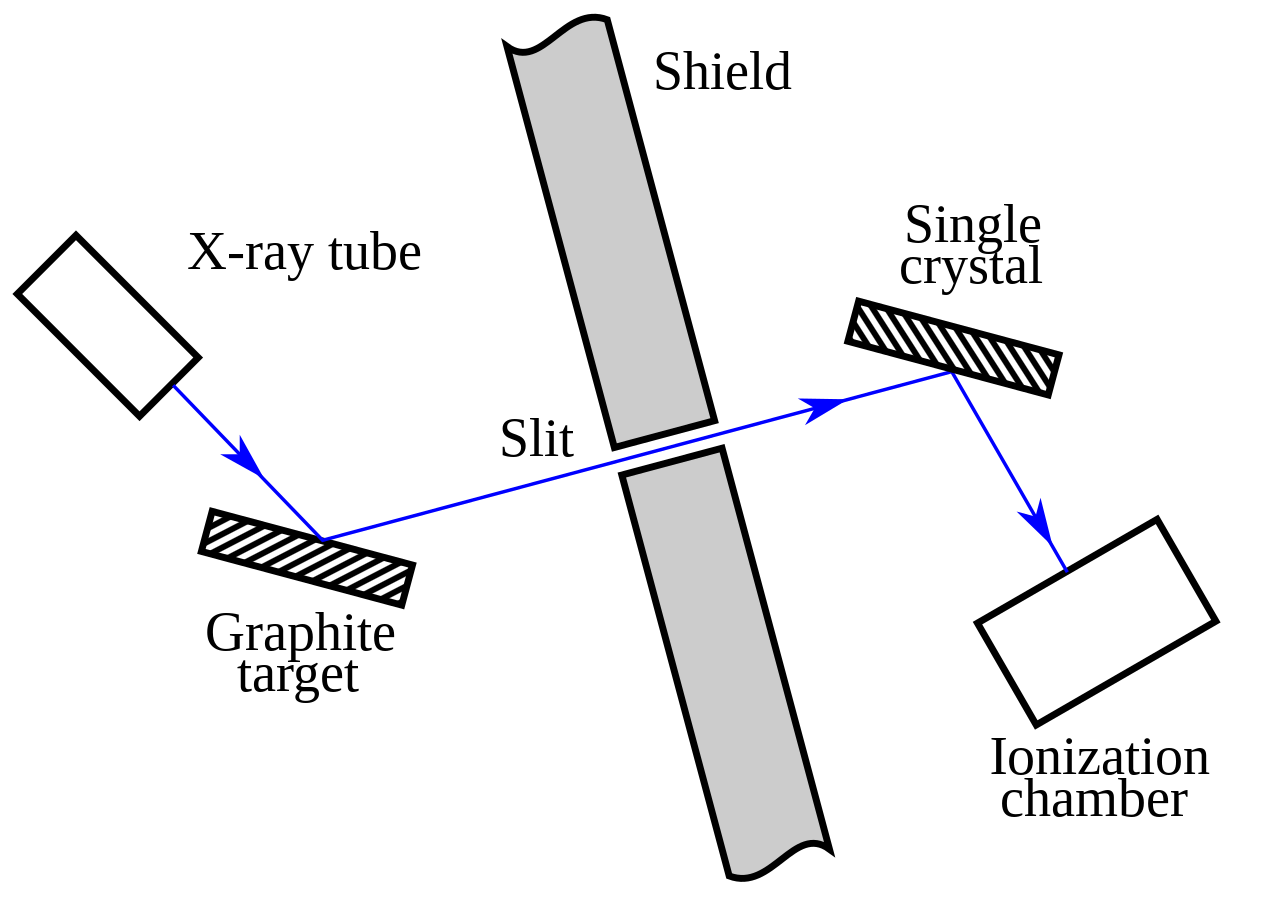
\includegraphics[width=0.45\columnwidth,alt={Schematic setup of Compton's experiment.}]{figures/compton1.png}%
\;~~~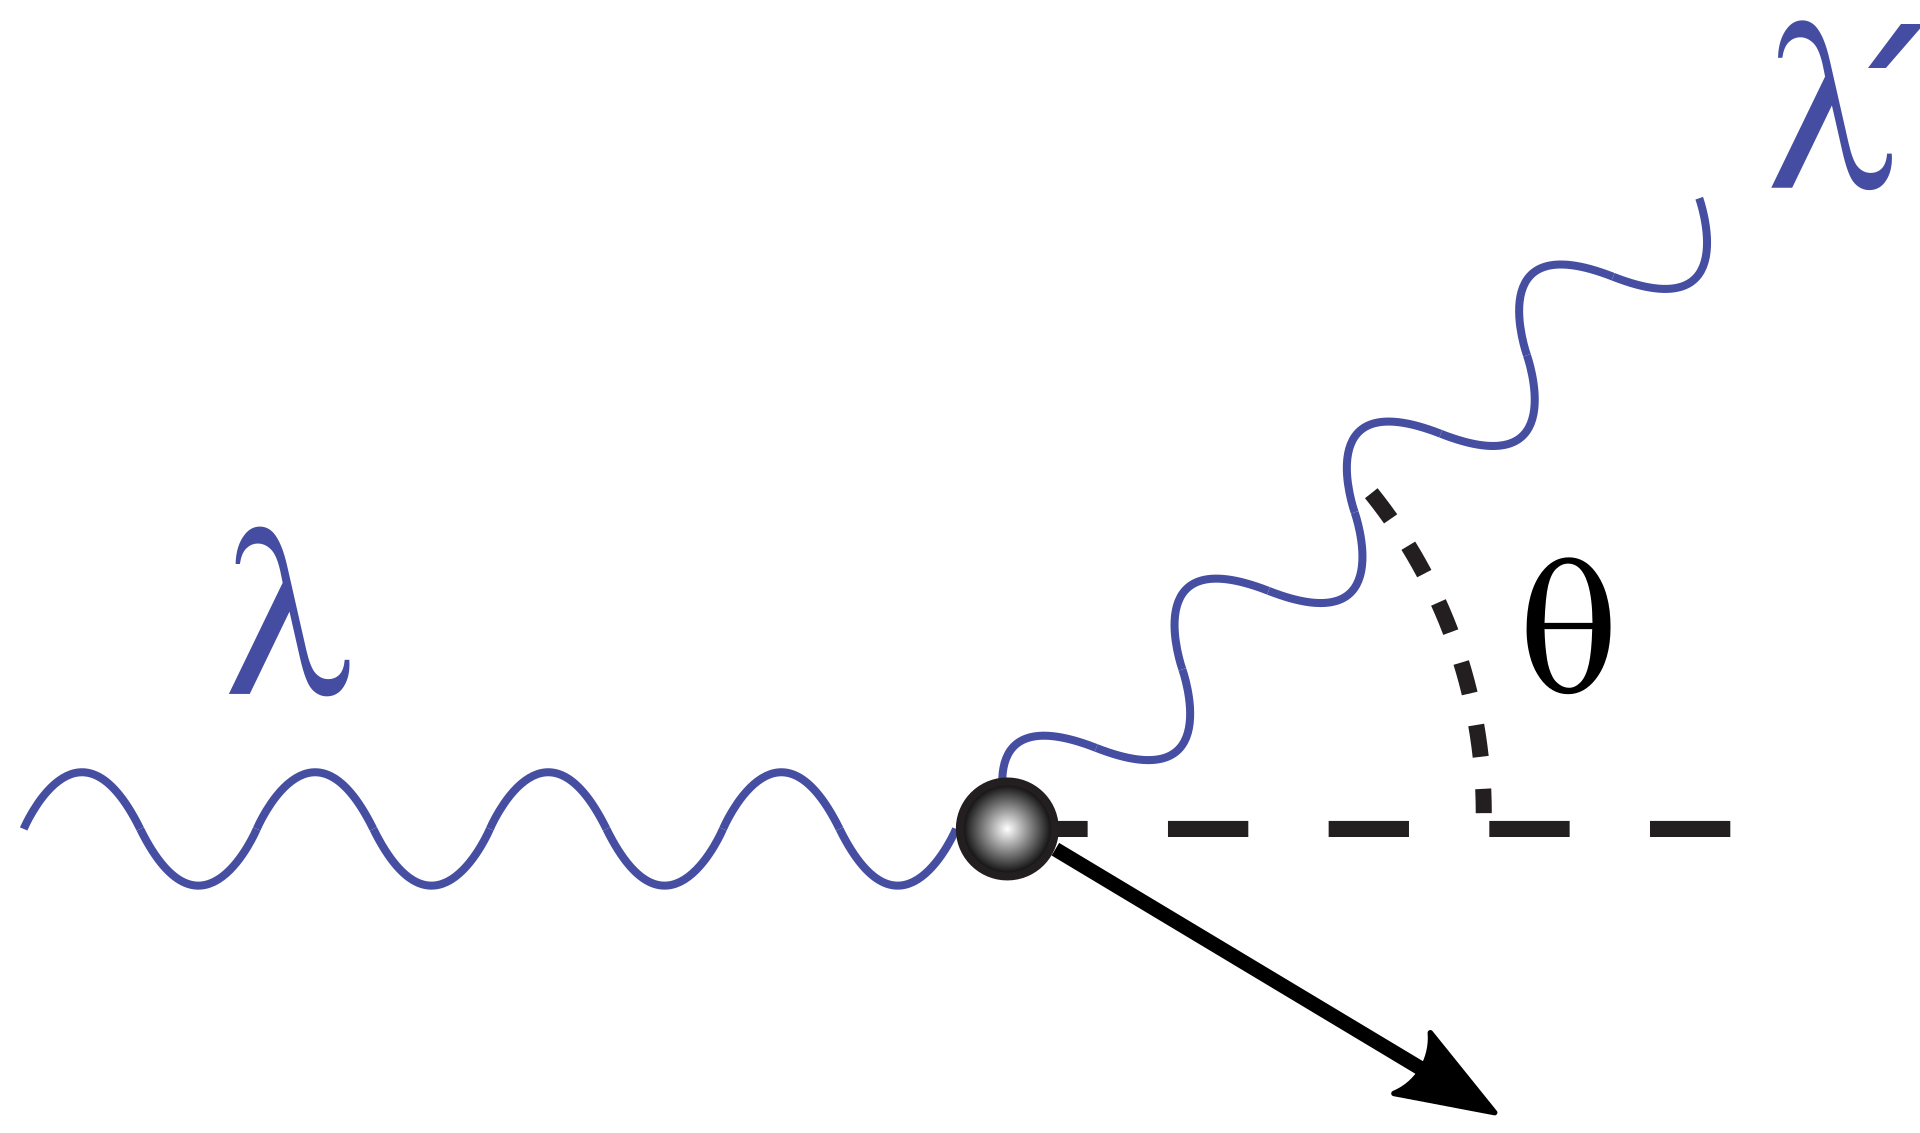
\includegraphics[width=0.45\columnwidth,alt={Photon–electron scattering diagram used to explain the Compton effect.}]{figures/compton2.png}
\caption{(Left) Schematic setup of Compton's experiment. (Right) The light-electron scattering process in the Compton experiment.}
\label{fig:compton}
\end{figure}

Discovered by Arthur Compton in 1923\cite{Compton1923}, when the energy of the X ray photon ($\sim$17 keV) was significantly larger than the binding energy of the atomic electron, the electrons could be treated as being free after scattering. In this case, a \emph{Compton shift} between the wavelengths of injected light ($\lambda$) and the scattered light ($\lambda^\prime$) was observed to satisfy the following relation with the scattering angle $\theta$ (see Fig. \ref{fig:compton}):
\begin{align}
\lambda^\prime-\lambda=\frac{h}{m_ec}(1-\cos\theta)
\end{align}
where $h$ is the Planck's constant.

The Compton shift can be explained by energy and momentum conservation, by assuming the photon energy of $E=h\nu=hc/\lambda$. 


\subsection{Quantization of atomic energy levels}


\subsubsection{Rydberg formula for the spectral lines in a hydrogen atom}

After the discovery of dark lines in the spectrum of the sun at the beginning of 18th century, it was later realized that hot atomic gases absorb and emit light only at certain definite frequencies. Building on works of Balmer and others, Rydberg discovered the following rule\cite{Rydberg1890} for the frequency of emitted light from hydrogen gases:
\begin{align}\label{rydberg rule}
\nu=\frac c\lambda=cR_H(\frac1{n^2}-\frac1{m^2}),~~~m,n\in\mbz_+.
\end{align}
This clearly demonstrated the discreteness of atomic energy levels $E_n\propto\frac1{n^2}$, further motivating Bohr's theory of the hydrogen atom. 

\subsubsection{Franck-Hertz experiment}

In the Franck-Hertz experiment (1914) illustrated in Fig. \ref{fig:franck-hertz}, in a vacuum tube fitted with three electrodes (an electron-emitting, hot cathode; a metal mesh grid; and an anode), when a grid voltage is applied between the cathode and the anode, the electric current through the tube filled with thin mecury vapours, due to electrons that pass through the grid and reach the anode, is measured in the experiment. As shown in the middle figure, the current increases rapidly at low voltages, and then sharply drops almost back to zero at 4.9 V, with similar effects observed as 9.8 V and other multiples of 4.9 V. This can be understood by the quantized energy levels of mercury atoms. inside the single mercury droplet in the vacuum tube, as shown in Fig. \ref{fig:franck-hertz}.

\begin{figure}
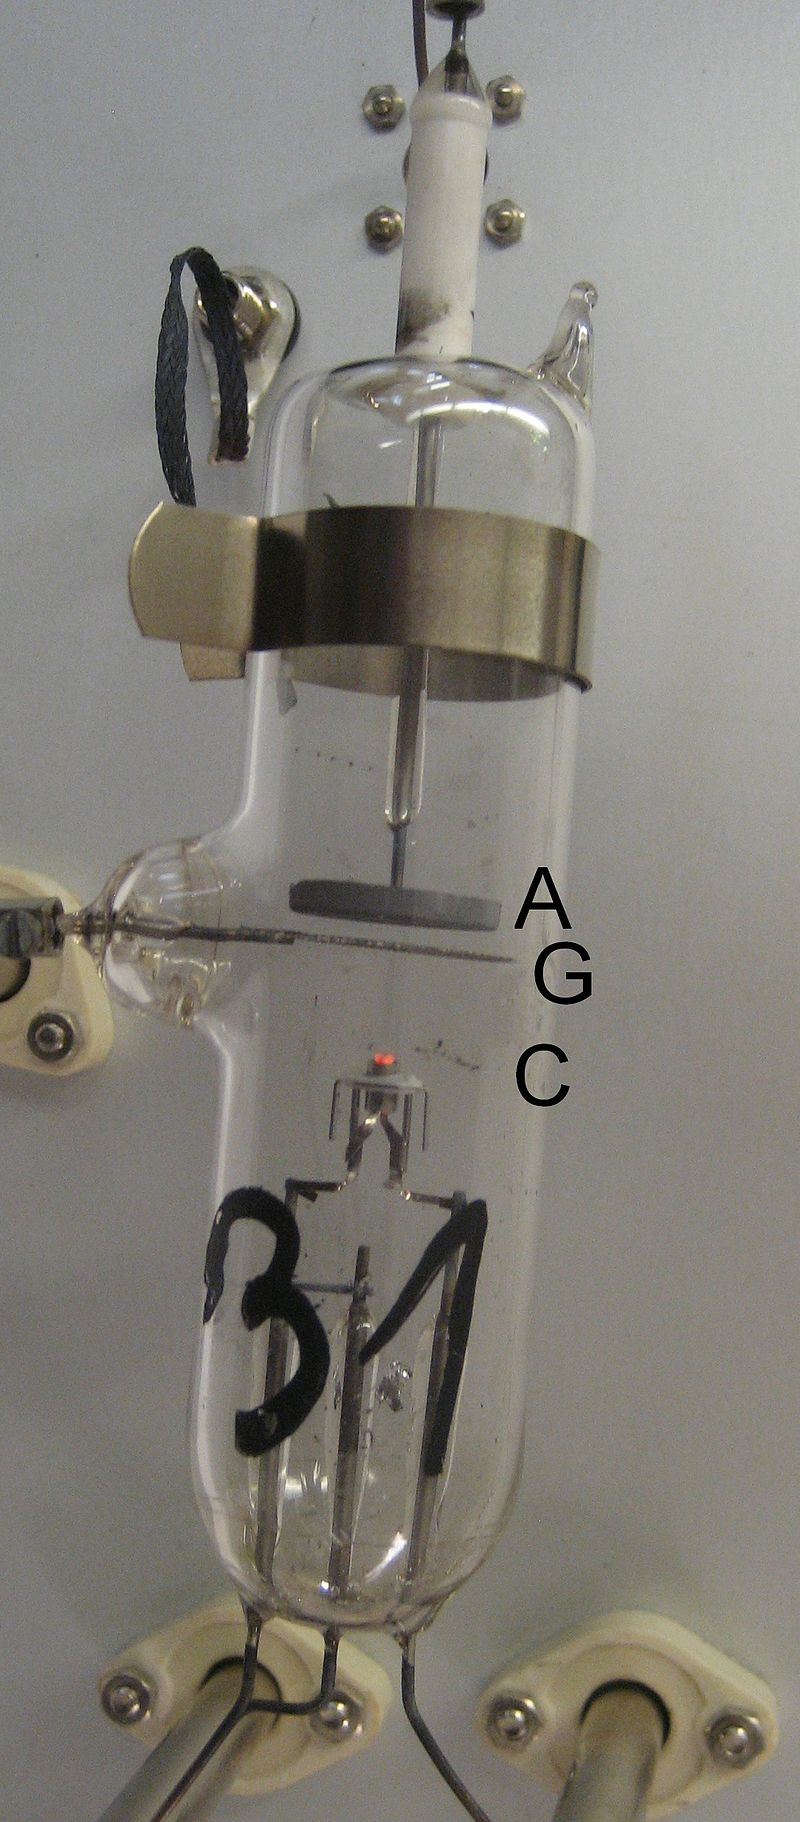
\includegraphics[width=0.2\columnwidth,alt={Photo of a vacuum tube used for the Franck–Hertz experiment.}]{figures/fh1.jpg}%
\;~~~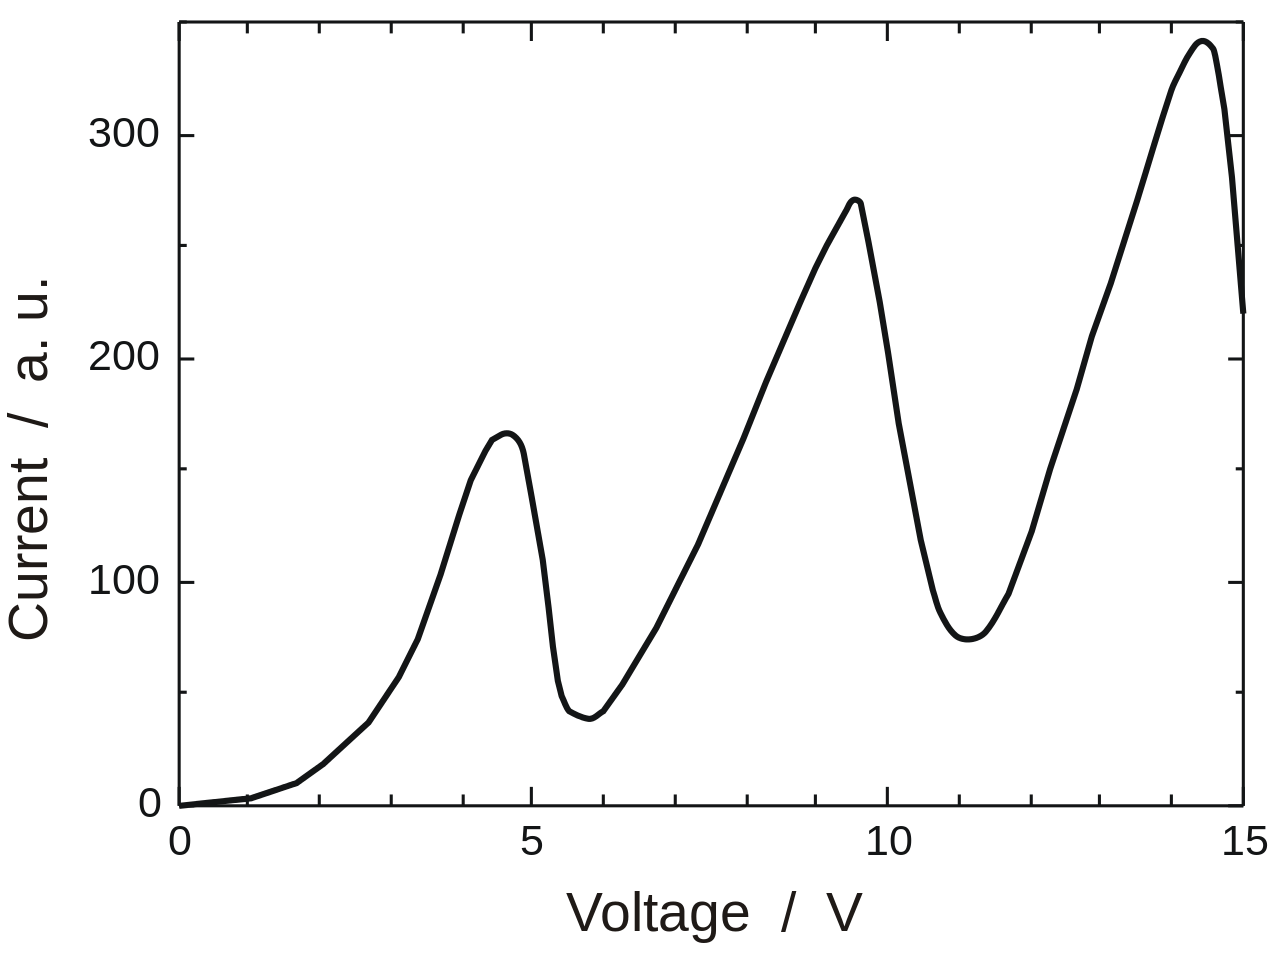
\includegraphics[width=0.45\columnwidth,alt={Anode current versus grid voltage showing peaks and drops at multiples of about 4.9 V.}]{figures/fh2.png}%
\;~~~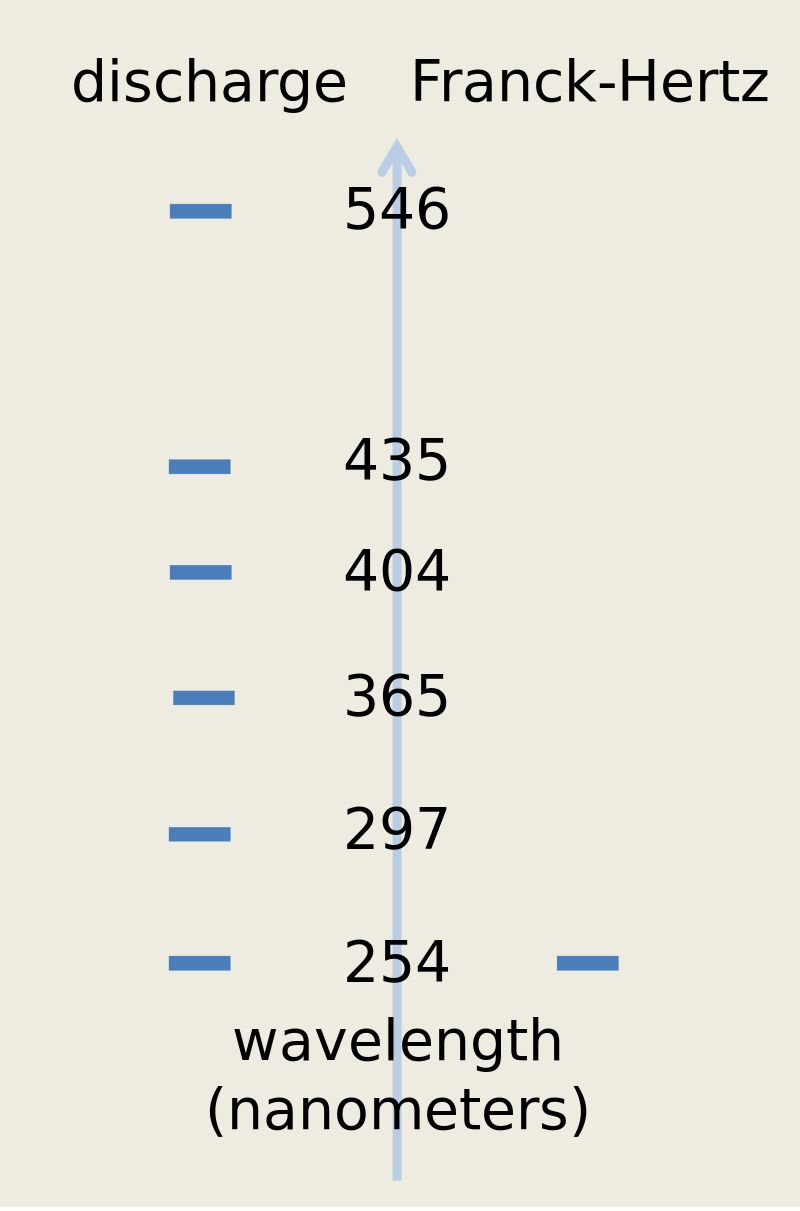
\includegraphics[width=0.25\columnwidth,alt={Mercury emission spectrum comparison for a discharge tube and a Franck–Hertz tube in operation.}]{figures/fh3.png}
\caption{(Left) Photograph of a vacuum tube used for the Franck-Hertz experiment. (Middle) Anode current (arbitrary units) versus the grid voltage relative to the cathode. (Right) Wavelengths of light emitted by a mercury vapor discharge and by a Franck-Hertz tube in operation at 10 V. (Picture from Wikipedia)}
\label{fig:franck-hertz}
\end{figure}



\subsection{Quantization of angular momentum}


\subsubsection{Bohr's explanation of hydrogen atom spectral lines}

Rydberg's rule\cite{Rydberg1890} indicates that the photon energy emitted by the hydrogen atom is given by
\begin{align}
h\nu=E_m-E_n,~~~E_n=-\frac{hcR_H}{n^2},~n\in\mbz_+.
\end{align}
How to explain the $1/n^2$ quantization of hydrogen atom energy levels? According to classical mechanics, for an electron in the Coulomb force field of hydrogen nucleus, its speed $v$ and radius $r$ satisfies
\begin{align}
\frac{mv^2}{r}=\frac{ke^2}{r^2}\Longrightarrow E=\frac12mv^2-\frac{ke^2}r=-\frac{ke^2}{2r}
\end{align}
where $k$ is the Coulomb constant. To fit the $n^2$ dependence of the orbit radius $r$, Niels Bohr came up with the following quantization condition for angular momentum:
\begin{align}
mvr=n\hbar
\end{align}
where $\hbar$ turns out to be $h/2\pi$. This quantization condition leads to the famous energy levels of electrons in a hydrogen atom:
\begin{align}
E_n=-\frac{mk^2e^4}{2\hbar^2}\frac1{n^2}=-\frac{13.6~\text{eV}}{n^2}
\end{align}

\subsubsection{Stern-Gerlach experiment demonstrated the quantization of angular momentum}

\begin{figure}
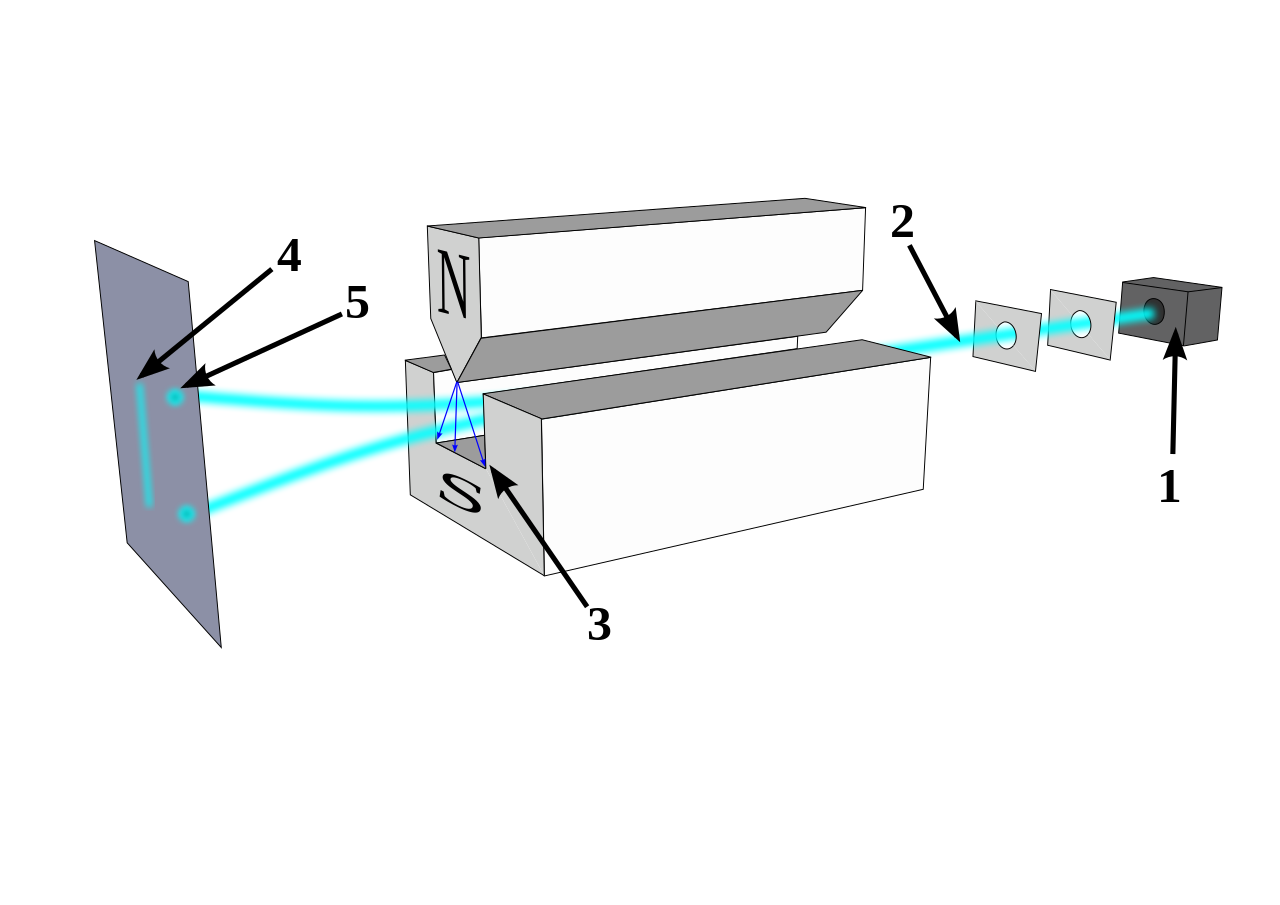
\includegraphics[width=0.8\columnwidth,alt={Stern–Gerlach apparatus showing a silver-atom beam split into two components in an inhomogeneous magnetic field.}]{figures/sg1.png}
\caption{Schematic setup of Stern-Gerlach experiment: Silver atoms travelling through an inhomogeneous magnetic field, being deflected up or down depending on their spin. (1) furnace, (2) beam of silver atoms, (3) inhomogeneous magnetic field, (4) the classically expected result, (5) the observed result.}
\label{fig:stern gerlach}
\end{figure}

In 1922 Stern and Gerlach performed an experiment\cite{Gerlach1922} measuring the deflection of silver atoms by an inhomogeneous magnetic field, as illustrated in Fig. \ref{fig:stern gerlach}. Due to the interaction energy $U=-\vec\mu\cdot\vec B$ of a magnetic moment $\vec\mu$ under a magnetic field $\vec B=B_z\hat z$, a non-uniform magnetic field exerts a force $\vec F=-\vec\nabla U=\mu_z\vec\nabla B_z$ on the moment-carrying silver atoms, therefore deflecting the silver atom beams in the inhomogenous magnetic field. As shown in Fig. \ref{fig:stern gerlach}, in contrast a continuous range of values of the magnetic moment as expected in classical mechanics, the experimental observations pointed to quantization of magnetic moment $\mu_z=g\mu_BS_z/\hbar$, where we defined $\mu_B$ as the Bohr magneton:
\begin{align}\label{Bohr  
   magneton}
\mu_B=\frac{\hbar e}{2m_e}
\end{align}
$g\approx 2$ as the electron $g$-factor and
\begin{align}
S_z=\pm\frac\hbar2
\end{align}
is the quantized spin angular momentum of a silver atom observed in Stern-Gerlach experiment.

This experiment demonstrated that in addition to energy level quantization, other physical observable such as spin angular momentum are also quantized in microscopic scales such as in silver atoms. Moreover, we can consider sequential Stern-Gerlach experiments shown in Fig. \ref{fig:stern gerlach sequentials}, where silver atoms are deflected by multiple inhomogeneous magnetic fields in a sequence. Remarkably, unlike the classical case of light passing through polarizers, which filter out everything after two polarizers with perpendicular polarization axes, two quantum mechanical ``beam splitters'' with perpendicular magnetic field directions still allows two splitted beams to pass through, as illustrated in the middle and bottom parts of Fig. \ref{fig:stern gerlach sequentials}.

\begin{figure}
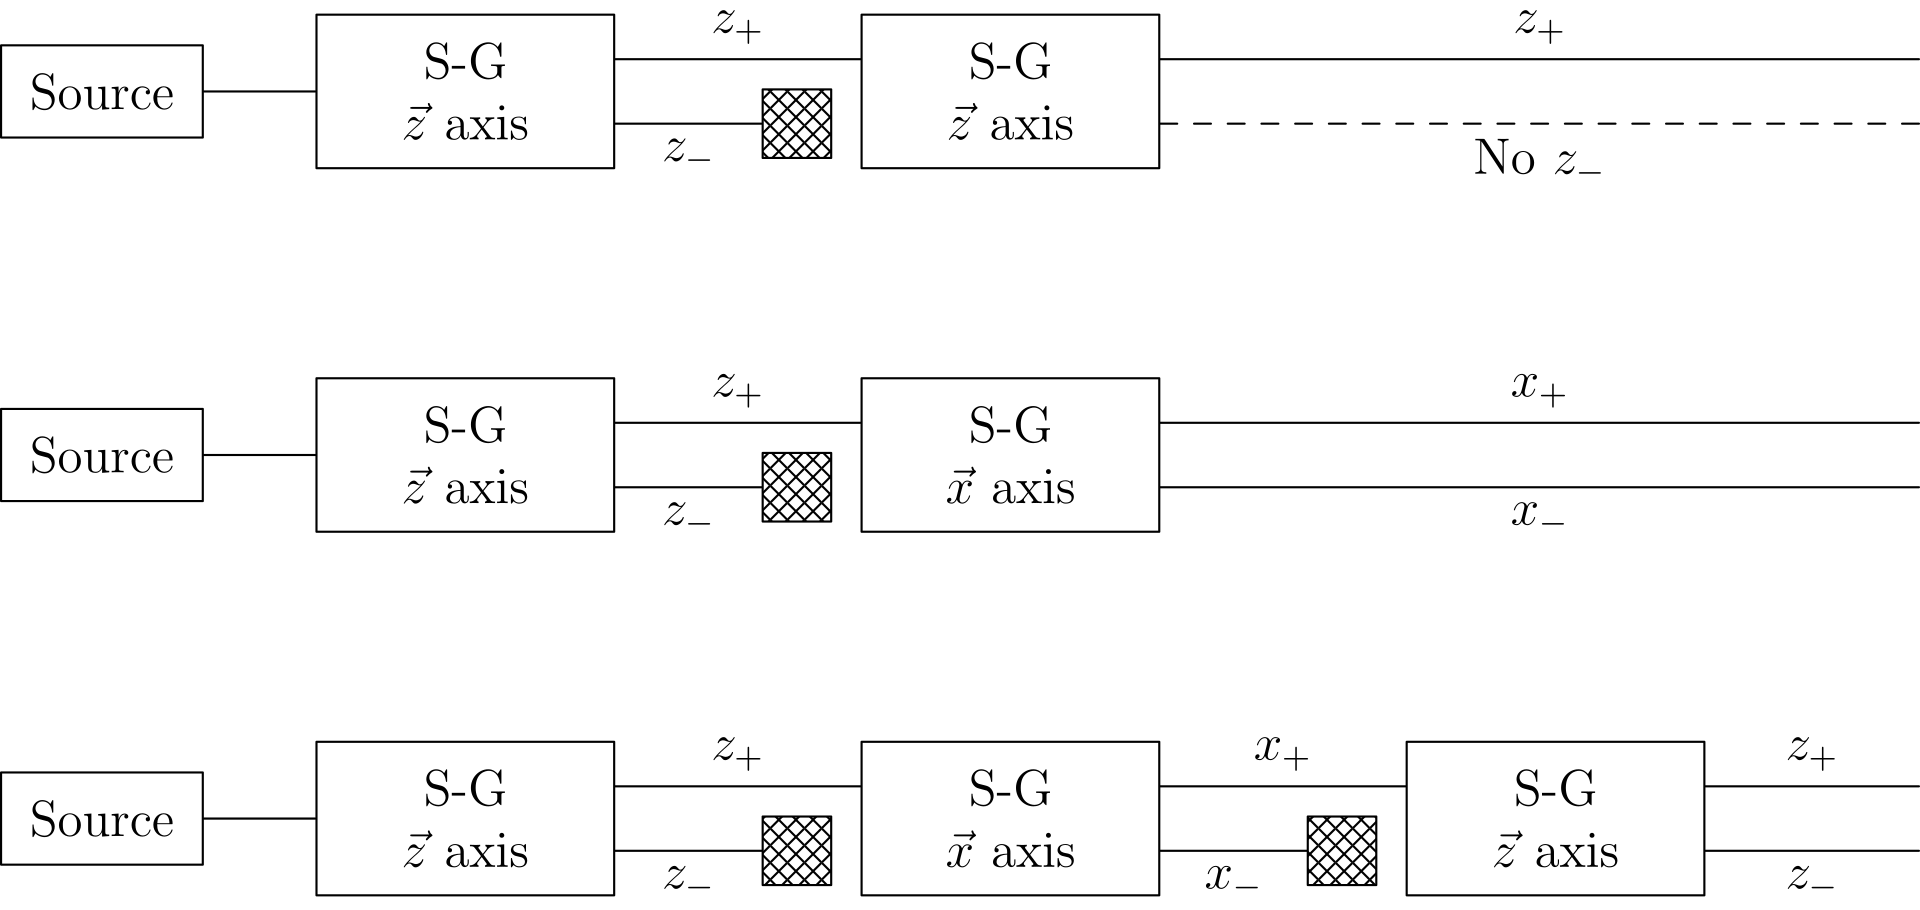
\includegraphics[width=0.9\columnwidth,alt={Sequential Stern–Gerlach setups illustrating outcomes for different magnetic-field orientations.}]{figures/sg2.png}
\caption{Sequential Stern-Gerlach experiments. (Picture from \sakurai)}
\label{fig:stern gerlach sequentials}
\end{figure}

\subsection{Davisson-Germer experiment demonstrated the wave nature of electrons}

In 1924 de Broglie formally proposed the wave nature of electrons and other particles, in terms of their de Broglie wavelengths:
\begin{align}\label{de Broglie wavelength}
\lambda=\frac{h}{p}
\end{align}
where $p$ is the momentum of the particle. If this proposal were true, it means that microscopic particles such as electrons should exhibit interference phenomena in the same way as acoustic and light waves. 

\begin{figure}
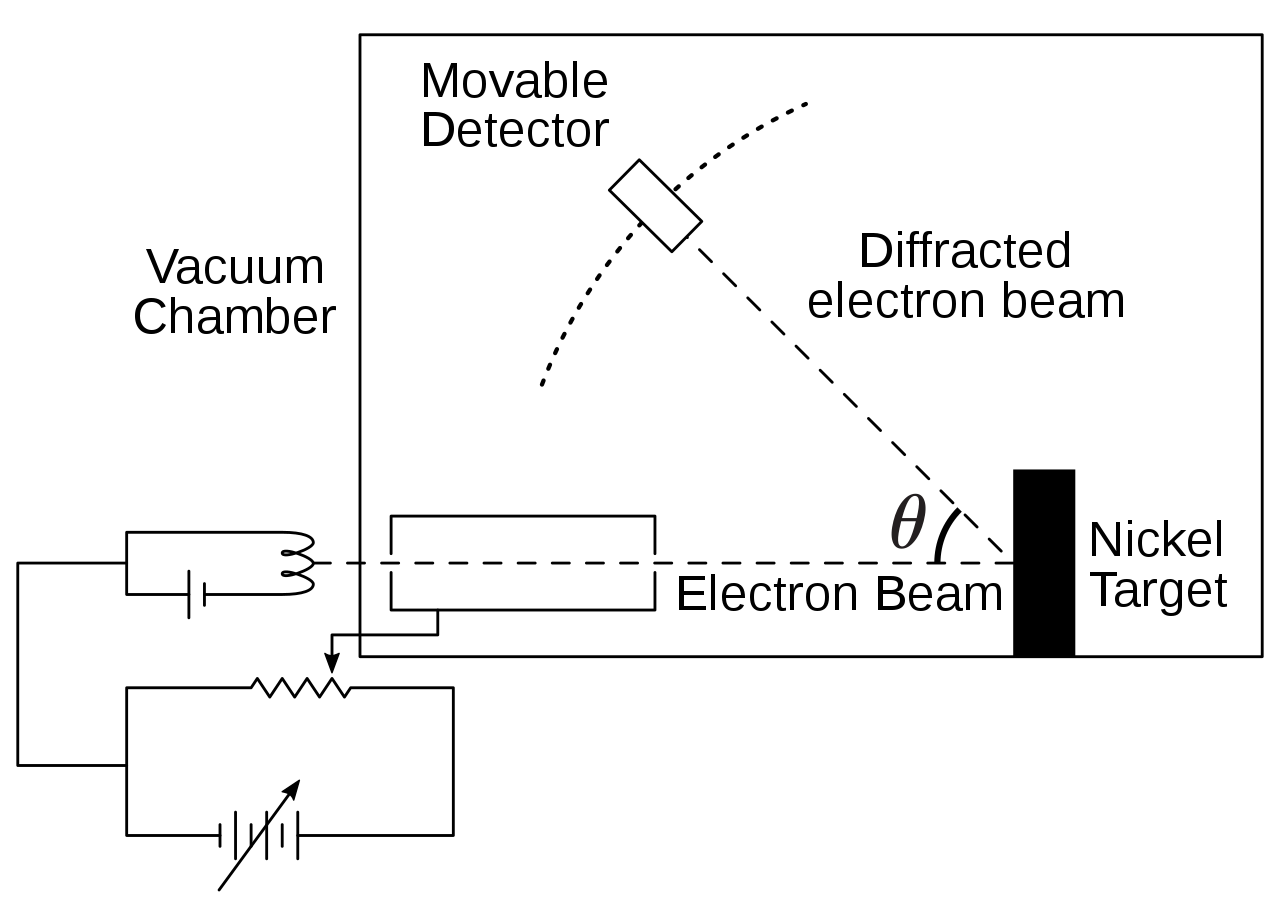
\includegraphics[width=0.45\columnwidth,alt={Davisson–Germer experimental setup schematic for electron diffraction from a crystal.}]{figures/dg1.png}%
\;~~~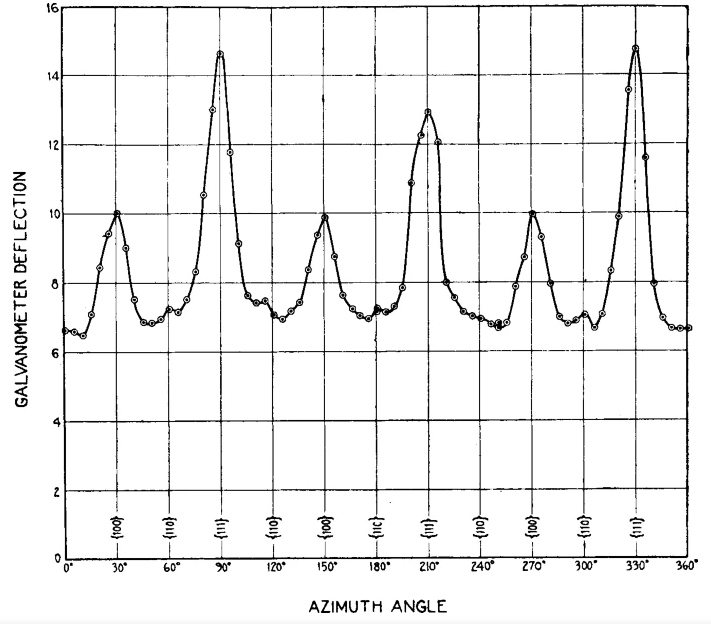
\includegraphics[width=0.4\columnwidth,alt={Plot of electron scattering intensity versus angle showing a diffraction peak at a given voltage.}]{figures/dg2.png}
\caption{(Left) Schematic setup of Davisson-Germer experiment. (Right) Intensity of electron scattering vs. azimuth angle at 54 volts, co-latitude $\theta=50^o$.}
\label{fig:davisson germer}
\end{figure}

In 1927 Davisson and Germer\cite{Davisson1927} performed an experiment to observe the diffraction pattern of electrons scattered by the surface of a crystal of nickel metal, as shown in Fig. \ref{fig:davisson germer}. The highest intensity was observed at an angle $\theta=50^o$ with a voltage of 54 V, giving the electrons a kinetic energy of 54 eV. To be compatible with the Bragg's law
\begin{align}\label{brag's law}
n\lambda=2d\sin(90^o-\theta/2),~~~n\in\mbz_+.
\end{align}
with the lattice spacing of nickel $d=0.091$ nm, the $n=1$ Bragg peak in (\ref{brag's law}) exactly corresponds to the de Broglie wavelength (\ref{de Broglie wavelength}) of electrons. We will examine the experimental results in Fig. \ref{fig:davisson germer} more carefully in Homework 1.
%\section{Hilbert space and state vectors (8/28)}

\referto{\nielsen~2.1, \tong~3.1, \shankar~1.1-1.4}

How to explain the above experimental observations? 4 postulates, derived (or more precisely, guessed) after a long process of trial and error, form the foundation for a theory framework that explains all observed experimental phenomena, known as quantum mechanics. Below we will introduce these postulates one by one, along the way of introducing linear algebra as the mathematics of quantum mechanics.

\begin{pos}\label{postulate 1}
    Associated to any isolated physical system is a complex vector space with inner product (i.e. a Hilbert space) known as the {state space} of the system. The system is completely described by its state vector, which is a unit vector in the system's state space.
\end{pos}

The key mathematical framework for quantum mechanics is linear algebra. The basic objects of linear algebra are vector spaces:

A \emph{vector space} over a \emph{scalar field} $\mathbb{F}$ is a set $\mathbb{V}$ of objects (called \emph{vectors}) equipped two binary operations: a \emph{vector addition} ($``+''$)
\begin{align}
\dket{v}+\dket{w}\in\mathbb{V},~~~\forall~\dket{v},\dket{w}\in\mathbb{V}.
\end{align}
and a \emph{scalar multiplication}:
\begin{align}
a\dket{v}\in\mathbb{V},~~~\forall~\dket{v}\in\mathbb{V},~a\in\mathbb{F}.
\end{align}
Mathematically, the set $\mathbb{V}$ forms an abelian group under vector addition operation and the scalar multiplication defines a ring homomorphism from the field $\mathbb{F}$ into the endomorphism ring of this abelian group. We will break down these terminology below. 

It is worthwhile to define a group since we will study symmetry in quantum mechanics later. A group is a set $V=\{u,v,\cdots\}$ equipped with a \emph{closed} binary operation $+$: $V\times V\rightarrow V$
\begin{align}
u+v=w\in V,~~~\forall~u,v\in V.
\end{align}
where 3 group axioms are satisfied:

(1) \emph{Identity element}:
\begin{align}
\exists~0\in V,~\text{s.t.}~\forall~u\in V,~u+0=0+u=u.
\end{align}

(2) \emph{Inverse}:
\begin{align}
\forall~u\in V,~\exists~(-u)\in V,~\text{s.t.}~u+(-u)=0.
\end{align}

(3) \emph{Associativity}:
\begin{align}
(u+v)+w=u+(v+w),~~~\forall~u,v,w\in V.
\end{align}
An Abelian group is a group whose addition operation is commutative:
\begin{align}
u+v=v+u,~~~\forall~u,v\in V.
\end{align}

The scalar multiplication is another map $\mathbb{F}\times\mathbb{V}\rightarrow\mathbb{V}$ that is \emph{associative}
\begin{align}
    a(b\dket{v})=(ab)\dket{v},~~~\forall~a,b\in\mathbb{F},~\dket{v}\in\mathbb{V}
\end{align}
and \emph{distributive in both the vectors and the scalars}:
\begin{align}
   &a(\dket{u}+\dket{v})=a\dket{u}+a\dket{v},\\
   &(a+b)\dket{v}=a\dket{v}+b\dket{v},~~~\forall~a,b\in\mathbb{F},~\dket{u},\dket{v}\in\mathbb{F}.
\end{align}
The above conditions satisfied by vector addition and scalar multiplication are summarized well in Chapter 1.1 of \shankar.

Of particular interests to quantum mechanics is a \emph{Hilbert space}, which is a ($n$-dimensional) vector space $\mathbb{C}^n$ over the field $\mathbb{C}$ of complex numbers, equipped with a map $\mathbb{V}\times\mathbb{V}\rightarrow\mathbb{C}$ known as an \emph{inner product}:
\begin{align}
\expval{u|v}\in\mathbb{C},~~~\forall~\dket{u},\dket{v}\in\mathbb{V}.
\end{align}
In the Dirac notation, $\dbra{u}$ is known as a \emph{bra}, and $\dket{v}$ is known as a \emph{ket}. The inner product is \emph{skew-symmetric}
\begin{align}
    \expval{u|v}=\expval{v|u}^\ast
\end{align}
\emph{positive semidefinite}
\begin{align}
    \expval{v|v}\geq0,~~~\expval{v|v}=0\Longleftrightarrow\dket{v}=0.
\end{align}
and \emph{linear in ket}
\begin{align}
    \dbra{u}(\sum_i\lambda_i\dket{v_i})=\sum_i\lambda_i\expval{u|v_i}
\end{align}
These properties are summarized in Chapter 1.2 of \shankar~and Chapter 2.1.4 of \nielsen.

Note that an inner product also defines a norm for each vector in vector space $\mathbb{V}$:
\begin{align}
|\dket{v}|\equiv\sqrt{\expval{v|v}}
\end{align}
Two important properties of an inner product are

(1) \textbf{ Cauchy-Schwarz inequality}:
\begin{align}
\expval{v|v}\expval{u|u}\geq|\expval{u|v}|^2
\end{align}
The equality holds if and only if $\dket{v}$ and $\dket{w}$ are linearly dependent.\\

(2) \textbf{ Triangle inequality} for the norms of vectors:
\begin{align}
|\dket{v}+\dket{w}|\leq|\dket{v}|+|\dket{w}|
\end{align}
Triangle inequality can be derived from the Cauchy-Schwarz inequality, which is a part of Homework 2. 

Strictly speaking, in addition to being a vector space equipped with an inner product (known as an inner product space), a Hilbert space must also be \emph{complete} in the sense that every Cauchy sequence $\{v^{(k)}\}$ of vectors in $\mathbb{V}$ has a limit that also lies in $\mathbb{V}$:
\begin{align}
\lim_{k\rightarrow\infty}v^{(k)}\in\mathbb{V},~~~\text{if}~\forall~\epsilon>0,~~~\exists~N\in\mbz_+,~\text{s.t.}~|v^{(m)}-v^{(n)}|<\epsilon,~~\forall~m,n>N.
\end{align}
For an inner product space of finite dimensions on any complete field $\mathbb{F}$, such as real and complex numbers $\mathbb{F}=\mathbb{R},\mathbb{C}$, it is automatically a Hilbert space. Below are a few examples of Hilbert spaces, and inner product spaces that are not Hilbert spaces:
\begin{itemize}
    \item $n$-dimensional Hilbert space on complex numbers: $\mathbb{V}\simeq \mathbb{C}^n$
    \item $n\times n$ complex matrices equipped with the Hilbert-Schmidt inner product forms a Hilbert space $L_{\mathbb{C}^n}$ (see Homework 1)
    \item $n$-dimensional Hilbert space on real numbers: $\mathbb{V}\simeq \mathbb{R}^n$
    \item $n$-dimensional vector space $\mathbb{V}\simeq \mathbb{Q}^n$ on rational numbers is not a Hilbert space because it is not complete, since a Cauchy sequence of rational numbers can converge to an irrational number.
    \item The inner product space of continuous square-integrable complex functions on interval $[a,b]$ with the following $L^2$ inner product:
    \begin{align}
   \expval{f_1|f_2}\equiv\int_a^bf_1^\ast(x)f_2(x)\text{d}x
    \end{align}
    is not a Hilbert space due to its incompleteness: a Cauchy sequence of continuous functions can be discontinuous. Its completion is the Hilbert space $L^2[a,b]$.
    \item For the same reason of incompleteness, the inner product space of polynomials on $[a,b]$ with the same $L^2$ inner product is not a Hilbert space, even though it's a subspace of $L^2[a,b]$.
\end{itemize}

A Hilbert space forms the \emph{state space} described in Postulate \ref{postulate 1}. With the help of the inner product structure, we can always choose a complete set of orthonormal basis $\{\dket{i}\}$ that expands the full state space $\mathbb{V}$, such that
\begin{align}
\dket{v}=\sum_iv_i\dket{i},~\forall~\dket{v}\in\mathbb{V};~~~\expval{i|j}=\delta_{i,j}
\end{align}
where $\delta_{i,j}$ is the Kronecker delta function. Given a $n$-dimensional vector space $V$, one can always find a set of $n$ linearly independent vectors $\{e_j|1\leq j\leq n\}$, known as a basis of vector space $V$, such that any vector $v\in V$ can be uniquely expressed as a linear superposition of the basis vectors: $v=\sum_{j}v_je_j$ with $v_j\in\mathbb{F}$. Given the inner product structure in a Hilbert space, a set of complete orthonormal basis can be constructed following the Gram-Schmidt procedure, discussed in details in Chapter 1.2 of \shankar~and Chapter 2.1.4 of \nielsen. In such a complete orthonormal basis of Hilbert space $\mathbb{V}=\mathbb{C}^n$, a Dirac ket $\dket{v}$ can be represented by a column vector $\vec v=(v_1,\cdots,v_n)^T$, a Dirac bra represented by a row vector, and the inner product reduces to the familiar form in $\mathbb{C}^n$:
\begin{align}
\expval{u|v}=\sum_iu_i^\ast v_i=\bpm u_1^\ast,\cdots,u_n^\ast\epm\bpm v_1\\ \cdots\\v_n\epm
\end{align}
%\section{Linear operators and observables (9/2)}

\referto{\nielsen~2.1; \tong~3.2, 4.1; \sakurai~1.3-1.4; \shankar~1.5-1.6}

Given two vector spaces $\mathbb{V}$ and $\mathbb{W}$, we can also define a linear operator $\hat O$ as any function that maps the vector space $\mathbb{V}$ to $\mathbb{W}$, which is linear in its inputs:
\begin{align}
\hat O(\sum_ia_i\dket{v_i})=\sum_ia_i\hat O(\dket{v_i})
\end{align}
In the case of $\mathbb{V}=\mathbb{W}$ we call it a linear operator $\hat O\in\mathbb{L}_\mathbb{V}$ on vector space $\mathbb{V}$, which is of particular interest to quantum mechanics.

Using a complete set of orthonormal basis $\{\dket{j}|1\leq j\leq\text{dim}\mathbb{V}\}$ for Hilbert space $\mathbb{V}$, each linear operator has a matrix representation:
\begin{align}
\hat O=\sum_{a,b}O_{a,b}\dket{a}\dbra{b},~~~O_{a,b}\equiv\expval{a|\hat O|b}
\end{align}
In particular, for the identity matrix which maps every vector to itself, we have the \textbf{completeness relation} for basis $\{\dket{i}\}$, also known as the \textbf{resolution of identity}:
\begin{align}
\sum_i\dket{i}\dbra{i}=\hat 1.
\end{align}
In the case of continuous variables, e.g. coordinates for a particle in free space, the summation will be replaced by integral:
\begin{align}
    \int\dif x\dket{x}\dbra{x}=\hat1
\end{align}
where $\dket{x}$ is an eigenstate of position operator $\dket{x}$ with eigenvalue $x$. 

We can also define the product of two linear operators $\hat M,\hat N\in\mathbb{L}_\mathbb{V}$:
\begin{align}
\hat M\hat N=\sum_{a,b,c}M_{a,b}N_{b,c}\dket{a}\dbra{c}
\end{align}
their commutator
\begin{align}
[\hat M,\hat N]=\hat M\hat N-\hat N\hat M
\end{align}
and anti-commutator
\begin{align}
\{\hat M,\hat N\}=\hat M\hat N+\hat N\hat M
\end{align}
and the \emph{Hermitian conjugate} (or \emph{Hermitian adjoint}) of an operator
\begin{align}
\hat O^\dagger=\sum_{a,b}O^\ast_{b,a}\dket{a}\dbra{b}=(O^T)^\ast=(O^\ast)^T
\end{align}
Specifically in Postulate \ref{postulate 3:projective measurements} about quantum (projective) measurements, each physical observable corresponds to a Hermitian linear operator, represented as a Hermitian matrix in the orthonormal basis:
\begin{align}
\hat M=\hat M^\dagger=\sum_{a,b}M_{a,b}\dket{a}\dbra{b},~~~(M^\dagger)_{a,b}=M^\ast_{b,a}=M_{a,b}\equiv\expval{a|\hat M|b}.
\end{align}

The diagonal form
\begin{align}\label{diagonal form}
\hat O=\sum_a O_a\dket{a}\dbra{a}
\end{align}
where $\{\dket{a}\}$ is a complete set of orthonormal basis of the Hilbert space, is also known as the \emph{spectral decomposition} of a matrix $\hat O$. If there is a complete set of orthonormal basis $\{\dket{a}\}$ such that the linear operator $\hat O$ can be rewritten as the diagonal form (\ref{diagonal form}), the matrix $\hat O$ is called ``diagonalizable''.

Not all matrices are diagonalizable (i.e. have a diagonal form), two non-diagonalizable examples are
\begin{align}
\hat M_1=\bpm1&1\\0&1\epm,~\hat M_2=\bpm1&1\\0&0\epm,~~~
\end{align}
$\hat M_1$ is known as a Jordan block with only 1 eigenvector, while $\hat M_2$ has two eigenvectors with different eigenvalues, but not orthogonal to each other. Generally, any complex square matrix can be decomposed into tensor sums of Jordan blocks by similarity transformations.\\

Below are a few useful theorems on the diagonalization of matrices:

\begin{thm}
    \textbf{The spectral decomposition theorem}: A linear operator $\hat O$ on vector space $\mathbb{V}$ is diagonal w.r.t. some orthonormal basis of $\mathbb{V}$ if and only if operator $\hat O$ is \emph{normal} i.e. $\hat O^\dagger\hat O=\hat O\hat O^\dagger$. 
\end{thm}
Refer to \nielsen~Box 2.2 for proof of this theorem.\\

\begin{thm}
    A normal matrix is Hermitian if and only if it has real eigenvalues.
\end{thm}

\begin{thm}
    The eigenkets corresponding to different eigenvalues of a Hermitian matrix are orthogonal.
\end{thm}

\begin{thm}
   A positive linear operator must be Hermitian. 
\end{thm}

\begin{thm}
    \textbf{Simultaneous diagonalization theorem}: Two Hermitian linear operators $\hat A$ and $\hat B$ can be diagnoalized simultaneously if and only if $[\hat A,\hat B]=0$.
\end{thm}
 In other words, there is a complete set of simultaneous eigenket $\{\dket{a,b}\}$ such that
\begin{align}
\hat A\dket{a,b}=a\dket{a,b},~~~\hat B\dket{a,b}=b\dket{a,b}.
\end{align}
if and only if $[\hat A,\hat B]=0$.\\

An Hermitian operator can be diagonalized into a special orthonormal basis $\{\dket{i}\}$, known as its eigenbasis, in which the linear operator is represented by a diagonal matrix
\begin{align}
\label{eigen basis}
\hat M=\sum_i\lambda_i\dket{i}\dbra{i}
\end{align}
If we use the set $\{m\}$ to label all different (real) eigenvalues of matrix $\hat M$, we can rewrite the above diagonal form (\ref{eigen basis}) as
\begin{align}
\hat M=\sum_m m\hat P_m,~~~\hat P_m=\sum_{j}\delta_{\lambda_j,m}\dket{j}\dbra{j}
\end{align}
where operators $\hat P_m$ are known as \emph{projection operators} (or \emph{projectors}) onto the eigenspace of $\hat M$ with eigenvalue $m$. Mathematically, a projector $\hat P$ is defined as a linear operator satisfying:
\begin{align}
\hat P^2=\hat P
\end{align}
You will learn more about projectors in HW2.

Given a state $\dket{\psi}$ and a physical observable $\hat M$, the (probability-weighted) \emph{expectation value} $\expval{\hat M}$ of operator $\hat M$ w.r.t. state vector $\dket{\psi}$ is
\begin{align}
\label{expval}
\expval{\hat M}\equiv\frac{\expval{\psi|\hat M|\psi}}{\expval{\psi|\psi}}
\end{align}
Naturally, the expectation value of any physical observable ia a real number, since any physical observable corresponds to a Hermitian operator.

We note that the expectation value (\ref{expval}) of any observable is the same for two linearly dependent states $\dket{\psi}$ and $\alpha\dket{\psi}$ for any complex scalar $\alpha\in\mathbb{C}$. This means $\dket{\psi}$ and $\alpha\dket{\psi}$ describe the same physical state. In other words, in a $N$-dimensional Hilbert space $\mathbb{V}=\mathbb{C}^N$, for a generic state
\begin{align}
\dket\psi\equiv\sum_{j=1}^N\psi_j\dket{j}
\end{align}
where $\{\dket{j}|1\leq j\leq N\}$ is a complete set of orthonormal basis of $\mathbb{V}$, although $\{\psi_j\in\mathbb{C}|1\leq j\leq N\}$ correspond to $2N$ independent real variables, only $2N-2$ of them are physically measurable, because the global phase factor and normalization leads to 2 redundancies that cannot be physically observed.

In the simplest example of a single qubit, we have $\mathbb{V}=\mathbb{C}^2$ for the $N=2$-dimensional Hilbert space. There are 4 linearly independent Hermitian operators in $\mathbb{C}^2$, whose matrix representations are
\begin{align}
\hat 1=\bpm1&0\\0&1\epm,~~~\hat\sigma_x=\bpm0&1\\1&0\epm,~~~\hat\sigma_y=\bpm0&-\imth\\ \imth&0\epm,~~~\hat\sigma_z=\bpm1&0\\0&-1\epm.
\end{align}
As you will learn in HW1, they (up to normalization) form a complete set of orthonormal basis for the Hilbert space $L_{\mathbb{C}^2}$ of linear operators. In the matrix representation, a generic state vector can be written as
\begin{align}
\dket{\psi}=\alpha\bpm\cos\theta e^{\imth\phi}\\ \sin\theta\epm,~~~\alpha\in\mathbb{C}
\end{align}
$\theta$ and $\phi$ are the two variables in the state vector that can be physically measured. One can carry out measurements for two observables to extract $\theta$ and $\phi$:
\begin{align}
\expval{\hat\sigma_z}=\cos(2\theta),~~~\expval{\hat\sigma_x}=\sin(2\theta)\cos\phi
\end{align}

\subsection{Appendix: Functions of operators/matrices}
\label{app:function of matrices}

A function $f(\hat M)$ of a square matrix $\hat M$ can be defined by the following Taylor expansion
\begin{align}
f(\hat M)=\sum_{n=0}^\infty\frac{\hat M^n}{n!}\frac{\text{d}^nf(x)}{\text{x}^n}|_{x=0}
\end{align}
if the Taylor expansion converges at $x=0$. In quantum mechanics we will mostly encounter square matrices that can be diagonalized, such as Hermitian and unitary matrices. 

For a diagonalizable matrix $\hat M$ with eigenkets $\{\dket{j}\}$ and eigenvalues $\{\lambda_j\}$, the matrix can be written as
\begin{align}
\hat M=\sum_j\lambda_j\dket{j}\dbra{j}
\end{align}
and a function of this diagonalizable matrix can be defined as
\begin{align}
f(\hat M)=\sum_jf(\lambda_j)\dket{j}\dbra{j}
\end{align}
%\section{Projective measurements (9/4)}

\referto{\nielsen~2.2.5, 2.2.7, \tong~3.4, 4.2, 16.4.1}

\begin{pos}\label{postulate 3:projective measurements}
    A \textbf{projective measurements} is described by a physical observable, $\hat M=\hat M^\dagger$ on the Hilbert space of the system being observsed. The observable has a specral decomposition
    \begin{align}
\hat M=\sum_m m\hat P_m
    \end{align}
    where $\hat P_m$ is the projector onto the eigenspace of $M$ with eigenvalue $m$. The possible outcomes of the measurement correspond to the eigenvalues $m$ of the observable. Upon measuring state $\dket{\psi}$, the probability of getting result $m$ is given by
    \begin{align}
p(m)=\expval{\psi|\hat P_m|\psi}
    \end{align}
    If the outcome $m$ occured, the state of the quantum system collapsed into a new state
    \begin{align}
    \hat P_m\dket{\psi}/\sqrt{p(m)}
    \end{align}
    immediately after the measurement.
\end{pos}

Postulate \ref{postulate 3:projective measurements} is in fact only a special form of quantum measurements, which will be discussed in detail in later parts of this course. Most generally, a generalized quantum measurement is described as follows:

\textbf{Postulate 2b}: A \textbf{generalized quantum measurement} is described by a collection $\{M_m\}$ of measurement operators. These are operators acting on the state space of the system being measured. The index $m$ refers to the measurement outcomes that may occur in the experiment. If the (normalized) state of the quantum system is $\dket{\psi}$ immediately before the measurements, then the probability that result $m$ occurs is given by
    \begin{align}
    p(m)=\expval{\psi|M_m^\dagger M_m|\psi}
    \end{align}
    and the state of the system after the measurement is $\frac{M_m\dket{\psi}}{\sqrt{\expval{\psi|M_m^\dagger M_m|\psi}}}$. The measurement operators satisfy the completeness equation
    \begin{align}\label{completeness equation}
    \sum_mM_m^\dagger M_m=\hat 1.
    \end{align}

When we choose $\hat M_m$ to be projector $\hat P_m$ into the eigenspace of observable $\hat M$ with eigenvalue $m$, the above generalized measurement reduces to the a projective measurement. Now it also becomes clear that the expectation value of observable $\hat M$ w.r.t. to (normalized) state vector $\dket{\psi}$ is nothing but the probability-weighted average of measurement outcomes:
\begin{align}
\expval{\hat M}\equiv\expval{\psi|\hat M|\psi}=\sum_m m\times p(m)
\end{align}
One can also find out the \emph{standard deviation} of measuring observable $\hat M$ in state $\dket{\psi}$:
\begin{align}
\Delta(M)\equiv\sqrt{\expval{(\hat M-\expval{\hat M})^2}}=\sqrt{\expval{\hat M^2}-\expval{\hat M}^2}
\end{align}

A significant consequence of the collapse part in Postulate \ref{postulate 3:projective measurements} is the following: starting from any state vector $\dket{\psi}$, if we measure the same observable $\hat M$ multiple times, the measurement outcome does not change any more after the 1st measurement. This is because the state already collapse into an eigenstate of $\hat M$ with some eigenvalue $m$ after the 1st measurement.

Another interesting aspect comes from \emph{incompatible measurements} of physical observables that do not commute with each other. If we perform two measurements $\hat A$ and $\hat B$ that satisfy $[\hat A,\hat B]\neq0$, for a generic quantum state, the measurement outcome depend on the order of the two measurements: i.e. measuring $\hat A$ after $\hat B$ versus $\hat B$ after $\hat A$ will yield different results. For example, starting from the eigenstate $\dket{\uparrow}$ of Pauli matrix $\sigma_z$, if we measure $\sigma_z$ and then $\sigma_x$, there is a probability of $1/2$ for us to end up with $+1$ outcomes for both measurements. However, if $\sigma_x$ is measured before the $\sigma_z$ measurement, there is only a probability of $1/4$ of $+1$ outcomes for both measurements.
%\section{Unitary evolution of a closed quantum system (9/9)}

\referto{\sakurai~2.1; \tong~3.3; \nielsen~2.1.8, 2.2.2, 4.2; \shankar~4.3}

In addition to Postulates \ref{postulate 1} and \ref{postulate 3:projective measurements} introduced earlier, we have two more postulates, one regarding how a quantum system evolves with time:
\begin{pos}\label{postulate 2}
    The time evolution of the state of a closed quantum system is described by the Schrodinger equation:
    \begin{align}\label{schrodinger eq}
    \imth\hbar\frac{\text{d}\dket{\psi}}{\text{d}t}=\hat H\dket{\psi}
    \end{align}
    where $\hbar=h/2\pi\approx1.05\times10^{-34}$ J$\cdot$s is a constant, and $\hat H$ is a fixed Hermitian operator known as the Hamiltonian of the closed system.
\end{pos}

Postulate \ref{postulate 2} states that the state vector associated with a closed quantum system evolves following the Schrodinger equation (\ref{schrodinger eq}). This postulate can be states in an equivalent manner:

\textbf{Postulate 3a} \emph{The evolution of a closed quantum system is described by a unitary transformation. That is, the state $\dket{\psi(t_2)}$ of the system at time $t_2$ is related to the state $\dket{\psi(t_1))}$ at time $t_1$ by a unitary operator $U$ which only depends on the times $t_1$ and $t_2$:}
\begin{align}
\dket{\psi(t_2)}=U(t_1,t_2)\dket{\psi(t_1)},~~~U(t_1,t_2)=e^{-\imth(t_2-t_1)\hat H/\hbar}
\end{align}
One can further generalize this to a time-dependent Hamiltonian $\hat H(t)$ where we have
\begin{align}
U(t_1,t_2)=\mathcal{T}e^{-\imth\int_{t_1}^{t_2}\hat H(t)\text{d}t/\hbar}
\end{align}
where $\mathcal{T}$ denotes time ordering in the integral, as explained in \sakurai~2.1.

In linear algebra, a unitary operator $\hat U$ is defined as any linear operator satisfying
\begin{align}
\hat U^\dagger\hat U=\hat 1.
\end{align}
which also implies $\hat U\hat U^\dagger=\hat 1$. Due to the spectrum decomposition theorem, a unitary operator can be diagonalized, and its eigenvalues all have modulus 1:
\begin{align}
\hat U\dket{\psi}=e^{\imth\theta}\dket{\psi}
\end{align}

\begin{table}[t]
\centering
\begin{tabular}{|c|c|c|}
\hline
Single-qubit gate&Symbol&Unitary matrix\\
\hline
Pauli-X (bit flip)&$X$&$\bpm0&1\\1&0\epm$\\
\hline
Pauli-Y&$Y$&$\bpm0&-\imth\\ \imth&0\epm$\\
\hline
Pauli-Z (phase flip)&$Z$&$\bpm1&0\\0&-1\epm$\\
\hline
Hadamard&$H$&$\frac1{\sqrt2}\bpm1&1\\1&-1\epm$\\
\hline
Phase&$S$&$\bpm1&0\\0&\imth\epm$\\
\hline
$\pi/8$&$T$&$\bpm1&0\\0&e^{\imth\pi/4}\epm$\\
\hline
\end{tabular}
\caption{Common single-qubit gates and associated unitary matrices.}\label{tab:single qubit gate}
\end{table}

Three examples of unitary operators in quantum mechanics are the following: (1) unitary time evolution operator $U(t_1,t_2)=e^{-\imth(t_2-t_1)\hat H/\hbar}$ for a closed quantum system discussed above; (2) a symmetry operator in a quantum system as we will discuss later in this course; (3) a quantum (logic) gate in quantum computing. For instance, in a two-dimensional closed quantum system, also known as a qubit, the common quantum gates are summarized in Table \ref{tab:single qubit gate}.

Starting from a complete set of orthonormal basis vectors $\{\dket{i}\}$ of Hilbert space $\mathbb{V}$, after the action of a unitary operator $\hat U$, we can obtain another complete set of orthonormal basis vectors $\{\dket{i}^\prime=\hat U\dket{i}\}$ of the same Hilbert space. In other words, each unitary operator implements a change of basis in the Hilbert space. Therefore, the unitary time evolution merely performs a rotation for vectors in the Hilbert space, since it only changes the state itself but not the inner product of any two states.  

In the case of unitary time evolution $U(t_1,t_2)$, the Hamiltonian $\hat H$ of a closed quantum system plays a crucial role. In its spectral decomposition:
\begin{align}
\hat H=\sum_aE_a\dket{a}\dbra{a}
\end{align}
the eigenkets $\dket{a}$ are called the \emph{energy eigenstates}, or \emph{stationary states}, and the eigenvalue $E_a$ is called the energy of state $\dket{a}$. In particular, the eigenstate with the lowest energy is known as the \emph{ground state}, while other states with higher energy are known as \emph{excited states}. According to Schrodinger equation (\ref{schrodinger eq}), a generic state vector
\begin{align}
\dket{\psi}=\sum_ac_a\dket{a}
\end{align}
evolves as
\begin{align}
\dket{\psi(t)}=e^{-\imth t\hat H/\hbar}\dket{\psi}=\sum_ac_ae^{-\imth E_at/\hbar}\dket{a}
\end{align}
and the different oscillation frequency $\omega_a=E_a/\hbar$ in different components of state $\dket{\psi(t)}$ can result in oscillations of physical observables. Two such examples, i.e. (1) spin precession; and (2) neutrino oscillation are discussed in detail in \sakurai~2.1, and will be a part of HW3. In particular, a physical observable you will encounter a lot in the future is the \emph{transition probability}:
\begin{align}
P(i\rightarrow f)\equiv|\expval{f|e^{-\imth\hat Ht/\hbar}|i}|^2
\end{align}
which measures the probability that an initial state $\dket{i}$ evolves into a final state $\dket{f}$ after time $t$. This quantity is directly related to the outgoing beam intensity in scattering experiments.

The transition probability is the modulus square of the \emph{propagator}
\begin{align}
    G(i,f:t)\equiv\expval{f|e^{-\imth\hat Ht/\hbar}|i}
\end{align}
which plays very important conceptual and computational roles in quantum mechanics. We will learn more about the propagator in HW3. 

\subsection{Schrodinger vs. Heisenberg pictures}

Regarding the time dependence of physical observables, such as the expectation value of a Hermitian operator $\hat O$ at time $t$, there are two equivalent ways to approach this problem. 

In the Schrodinger picture, where the state vector $\dket{\psi}$ evolves with time while the operator $\hat O$ remains a constant:
\begin{align}
    \dket{\psi_S(t)}=\hat U(t,0)\dket{\psi_0},~~~\hat O_S(t)=\hat O
\end{align}
In the Heisenberg picture, on the other hand, the state vector remains a constant while the operator evolves with time:
\begin{align}
    \dket{\psi_H(t)}=\dket{\psi_0},~~~\hat O_H(t)=\hat U^\dagger(t,0)\hat O\hat U(t,0)
\end{align}
It is straightforward to show that both pictures yield the same physical observable
\begin{align}
    \expval{O(t)}=\expval{\psi_S(t)|\hat O_S(t)|\psi_S(t)}=\expval{\psi_H(t)|\hat O_H(t)|\psi_H(t)}=\expval{\psi_0|\hat U^\dagger(t,0)\hat O\hat U(t,0)|\psi_0}
\end{align}

In general, it is more convenient to use the Heisenberg picture to compute expectation values of an observable, while the Schrodinger picture is more convenient to extract time dependence of the state vector and its related properties, such as entanglement entropy.

\subsection{Quantum Zeno effect}

Consider a quantum system under repeated measurements of a physical observable $\hat O$ with the following spectral decomposition:
\begin{align}
    \hat O=\sum_q q~\dket{q}\dbra{q}
\end{align}
Without loss of generality, let's assume the initial state of the system is $\hat O$ eigenstate $\dket{0}$ with eigenvalue $q_0$. 

Now consider a generic Hamiltonian
\begin{align}
    \hat H=H_{0,0}\dket0\dbra0+\sum_{q\neq0}(H_{q,0}\dket{q}\dbra0+h.c.)+\sum_{p,q\neq0}H_{p,q}\dket{p}\dbra{q}
\end{align}
that governs the time evolution of the system. We used $h.c.$ as a shorthand notation for ``hermitian conjugate''. 

Starting from the initial state $\dket0$, after a very short time $\Delta t$, the state evolves into
\begin{align}
    \dket{\psi(t)}=e^{-\imth \hat Ht/\hbar}\dket0=(1-\frac\imth\hbar H_{0,0}\Delta t)\dket0-\frac\imth\hbar\Delta t\sum_q H_{q,0}\dket{q}+O(\Delta t^2)
\end{align}
Therefore at time $\Delta t$, the probability of measurement outcome $\hat O=q_0$ is given by
\begin{align}
    |\expval{0|\psi(t)}|^2=1-\alpha(\Delta t)^2+O(\Delta t^3),~~~\alpha>0
\end{align}
where the constant $\alpha$ depends on the Hamiltonian $\hat H$. 

One can further show that if we repeat this 2-step procedure of small time evolution for $\Delta t=\frac TN$ followed by a measurement of operator $\hat O$, after $N$ repetitions, the probability for the state to come back to itself approaches 1 in the large $N$ limit:
\begin{align}
    \text{Pr}(\dket{0}\rightarrow\dket0)\geq\lim_{N\rightarrow\infty}\big(|\expval{0|\psi(\frac TN)}|^2\big)^N=\lim_{N\rightarrow+\infty}e^{-\alpha T^2/N}=1
\end{align}
This is known as the quantum Zeno effect. 
%\section{Composite quantum systems and tensor product (9/11)}
\label{sec:composite system}

\referto{\nielsen~2.1.7, 2.2.8, 4.3; \tong~3.6}

Previously we have focused on a single closed quantum system. When two closed quantum systems are combined together e.g. through some interactions b/w the two systems, how to describe such as composite quantum system? The last postulate addresses this issue, under the mathematical frameworks of \emph{tensor product}:
\begin{pos}\label{postulate 4}
    The state space of a composite physical system is the tensor product of the state spaces of the component physical systems. Moreover, if we have systems numbered 1 through $n$, and the system number $i$ is prepared in the state $\dket{\psi_i}$, then the joint state of the total system is $\dket{\psi_1}\otimes\dket{\psi_2}\otimes\cdots\otimes\dket{\psi_n}$.
\end{pos}

Specifically, consider two quantum systems with Hilbert space $V$ of dimension $m$ and $W$ of dimension $n$, their composite system is described by the tensor product of the two Hilbert spaces:
\begin{align}
V\otimes W\equiv\{\dket{v}\otimes\dket{w}|\dket{v}\in V, \dket{w}\in W\}
\end{align}
which is a Hilbert space of dimension $mn$. Linear operators on $V\otimes W$ are given by $A\otimes B$, where $A$ is a linear operator on $V$ and $B$ is a linear operator on $W$, satisfying
\begin{align}
(A\otimes B)\dket{v}\otimes\dket{w}=A\dket{v}\otimes B\dket{w}
\end{align}
An inner product on $V\otimes W$ is naturally defined as
\begin{align}
(\sum_ia_i\dket{v_i}\otimes\dket{w_i},\sum_jb_j\dket{v_j^\prime}\otimes\dket{w_j^\prime})=\sum_{i,j}a^\ast_ib_j\expval{v_i|v_j^\prime}\expval{w_i|w_j^\prime}
\end{align}
One can therefore define a complete set of orthonormal basis $\{\dket{v_i}\otimes\dket{w_j}\}$ for $V\otimes W$, and the matrix representation of linear operators in $V\otimes W$ is given by
\begin{align}
(A\otimes B)_{i,j}=A_{i_1,j_1}B_{i_2,j_2},~~~A\in L_V,~B\in L_W.
\end{align}
Since $A\otimes B$ is a matrix of dimension $mn$, where $m$ and $n$ are dimensions of matrices $A$ and $B$ respectively, the row and column index of matrix $A\otimes B$ can be written as
\begin{align}
i=(i_1-1)n+i_2,~~~j=(j_1-1)n+j_2.
\end{align}
More properties of tensor product can be found in \nielsen~section 2.1.7.

\begin{table}[t]
\centering
\begin{tabular}{|c||c|c|c|}
\hline
Name&Controlled-Z (CPHASE)&CNOT&SWAP\\
\hline
Unitary matrix&$\bpm1&0&0&0\\0&1&0&0\\0&0&1&0\\0&0&0&-1\epm$&$\bpm1&0&0&0\\0&1&0&0\\0&0&0&1\\0&0&1&0\epm$&$\bpm1&0&0&0\\0&0&1&0\\0&1&0&0\\0&0&0&1\epm$\\
\hline
\end{tabular}
\caption{Common 2-qubit gates and associated unitary matrices.}\label{tab:2-qubit gate}
\end{table}

\begin{table}[t]
\centering
\begin{tabular}{|c||c|c|}
\hline
Name&Toffoli (Controlled-CNOT)&Fredkin (Controlled-SWAP)\\
\hline
Unitary matrix&$\frac{1+Z_1}2\otimes\text{CNOT}_{23}+\frac{1-Z_1}2\otimes\hat 1_{23}$&$\frac{1+Z_1}2\otimes\text{SWAP}_{23}+\frac{1-Z_1}2\otimes\hat 1_{23}$\\
\hline
\end{tabular}
\caption{Common 3-qubit gates and associated unitary matrices.}\label{tab:3-qubit gate}
\end{table}

With the help of tensor product, we can define Hamiltonian and unitary operators for a composite quantum system. We will study the transverse field Ising model for a 2-qubit system
\begin{align}
\label{tfim}
H_\text{TFIM}=-JX_1\otimes X_2-h(Z_1\otimes\hat 1_2+\hat 1_2\otimes Z_2)
\end{align}
as a demonstration. Due to a conserved quantity $Z_1\otimes Z_2$ that commutes with the Hamiltonian, it can be diagonalized in the $Z_1\otimes Z_2=\pm1$ subspaces respectively.

A good set of examples of unitary operators in a composite system are 2-qubit and 3-qubit quantum gates, shown in Table \ref{tab:2-qubit gate} and \ref{tab:3-qubit gate} respectively, such as a controlled-$U$ gate in the 2-qubit system.
\chapter{Density matrix formulation of quantum mechanics}
\label{chap:density matrix}



\section{Density matrix and mixed states (9/16)}\label{sec:schmidt decomposition}

\referto{\nielsen~2.4, 2.5; \tong~16.3.3, 16.4}


If we think of a physical system (with Hilbert space $A$) and its environment (with Hilbert space $B$) combined together as a (composite) closed quantum system, any state therein is described by a state vector
\begin{align}\label{system+environment}
\dket{\psi}=\sum_{i,j}\psi_{i,j}\dket{a_i}\otimes\dket{b_j}
\end{align}
where $\{\dket{a_i}|1\leq i\leq m=\text{dim}A\}$ is a complete set of orthonormal basis for $A$, while $\{\dket{b_j}|1\leq j\leq n=\text{dim}B\}$ is a complete set of orthonormal basis for $B$. 

To study physical properties of system $A$, the composite state $\dket\psi$ in (\ref{system+environment}) is an overkill because it also contains all information about the environment, in which we are not interested at all. It turns out the following quantity, known as the \emph{density matrix} (or \emph{density operator}) for subsystem $A$
\begin{align}\label{reduced density matrix}
\hat\rho=\trace_B\dket{\psi}\dbra{\psi}=\sum_{i_1,i_2=1}^{m}\rho_{i_1,i_2}\dket{a_{i_1}}\dbra{a_{i_2}},~~~\rho_{i_1,i_2}=\sum_{j=1}^n\psi_{i_1,j}\psi^\ast_{i_2,j}
\end{align}
encodes all information about physical system $A$ in composite state $\dket\psi$. As shown above it is obtained by tracing out subsystem $B$ in state $\dket\psi$. Any physical observable of the system $A$ corresponds to a Hermtian operator $\hat O_A\times\hat 1_B$ in the composite system $A\times B$, and its expectation value is nothing but
\begin{align}
    \expval{\hat O}_A\equiv\expval{\psi|\hat O_A\otimes\hat1_B|\psi}=\text{Tr}(\hat\rho\hat O)
\end{align}

Instead of directly computing the partial trace, there is another efficient way to obtain the density matrix (\ref{reduced density matrix}), known as \emph{Schmidt decomposition}, which we describe below. This approach is especially informative for understanding entanglement between subsystem $A$ and $B$. 

We can treat the wavefunction $\psi_{i,j}$ in (\ref{system+environment}) as a matrix of dimension $m\times n$, which has the following singular value decomposition (SVD):
\begin{align}
\psi=U^\dagger DV,~~~U^\dagger U=V^\dagger V=\hat 1,~~~D_{i,j}=\delta_{i,j}\lambda_i,~\lambda_i\geq0.
\end{align}
where $U,V$ are two unitary matrices of dimensions $m\times m$ and $n\times n$ respectively. $D$ is a $m\times n$ matrix whose matrix elements all vanish except for positive diagonal elements $\{\lambda_i>0|1\leq i\leq r,~r\leq\min({m,n)}\}$, known as singular values of matrix $\psi$. The positive integer $r\leq\min{(m,n)}$, is the rank of matrix $\hat\psi$. 

Since unitary matrices implement the change of basis, the SVD procedure introduced a new set of orthonormal basis (known as the Schmidt basis) for both the system $A$ and environment $B$:
\begin{align}
\dket{A_i}=\sum_{i^\prime}U^\ast_{i,i^\prime}\dket{a_{i^\prime}},~~~\dket{B_j}=\sum_{j^\prime}V_{j,j^\prime}\dket{b_{j^\prime}}
\end{align}
such that the state vector (\ref{system+environment}) can be written as
\begin{align}
\dket{\psi}=\sum_{i=1}^r\lambda_i\dket{A_i}\otimes\dket{B_i},~~~\lambda_i>0
\end{align}
This is known as the Schmidt decomposition of state vector $\dket{\psi}$ in a composite Hilbert space, which is the tensor product of $A$ and $B$. The rank $r$ of matrix $\psi$ is known as the Schmidt rank (or Schmidt number), and the positive numbers $\{\lambda_i>0|1\leq i\leq r\}$ are known as Schmidt coefficients. 



Note that normalization of state vector $\dket{\psi}$ implies that $\{p_i\equiv\lambda_i^2\}$ leads to a normalized probability distribution:
\begin{align}
\expval{\psi|\psi}=\sum_{i=1}^r\lambda_i^2=1=\sum_{i=1}^r p_i
\end{align}


In the Schmidt basis $\{\dket{A_i}\}$, the density matrix (\ref{reduced density matrix}) has the following diagonal form:
\begin{align}\label{ensemble of state}
\hat\rho=\sum_{i=1}^r\lambda_i^2\dket{A_i}\dbra{A_i}=\sum_{i=1}^rp_i\dket{A_i}\dbra{A_i}
\end{align}
which has the physical meaning as an ensemble $\{p_i,\dket{A_i}\}$ of pure states. $p_i$ is the probability for the system $A$ to fall into pure state $\dket{A_i}$. 

Mathematically, a density matrix is defined as a linear operator $\hat\rho$ satisfying 2 conditions:

(1) \textbf{Trace condition} 
\begin{align}
\trace\hat\rho=1
\end{align}

(2) \textbf{Positivity condition}
\begin{align}
\hat\rho\geq0
\end{align}
The positivity of $\hat\rho$ already implies that it is a Hermitian operator i.e. $\hat\rho=\hat\rho^\dagger$. 

All density matrices form a convex set in the sense that $x\rho_1+(1-x)\rho_2,~\forall~0\leq x\leq1$ is also a density matrix if $\rho_{1,2}$ are density matrices. 

In the diagonal basis (\ref{ensemble of state}) of density matrix $\hat \rho$, if the Schmidt rank $r>1$ i.e. there are at least two independent pure states in the ensemble, we call $\hat\rho$ a \emph{mixed state}. If $r=1$, instead we call $\hat\rho=\dket{A_1}\dbra{A_1}$ to be a \emph{pure state}. 
\begin{thm}
    A density matrix $\hat\rho$ corresponds to a pure state if and only if 
\begin{align}
    {\hat\rho}^2=\hat\rho
\end{align}
\end{thm}





As a simplest example of Schmidt decomposition, we consider a single-qubit physical system $A$ and a single-qubit environment $B$, where a pure state of the combined closed system has the following general form:
\begin{align}
\dket{\psi}=\alpha\dket{00}+\beta\dket{01}+\gamma\dket{10}+\delta\dket{11}
\end{align}
where we have used $\dket{0}\equiv\dket{\uparrow}$ and $\dket{1}\equiv\dket{\downarrow}$ (known as the computational basis) to label eigenstates of the Pauli-$\hat Z$ operator. We also used a shorthand notation for tensor product states:
\begin{align}
\dket{ab}\equiv\dket{a}_A\otimes\dket{b}_B,~~~a,b=0,1.
\end{align}
In this case we have the matrix $\psi_{a,b}$ as
\begin{align}
\hat\psi=\bpm \alpha&\beta\\ \gamma&\delta\epm
\end{align}
for the SVD procedure.  
\section{Entanglement and quantum teleportation (9/18)}

\referto{\nielsen~1.3.6-1.3.7, 2.4.3; \tong~16.2.3, 16.3.2, 16.3.4. Use \nielsen~11.3 for further readings on entropy.}

\subsection{Entanglement entropy}

In the Schmidt decomposition described in section {\ref{sec:schmidt decomposition}}, if the density matrix $\hat\rho$ is obtained by a partial trace over $B$ from state $\rho_{AB}$ in the composite system $A\otimes B$:
\begin{align}
\hat\rho_A=\trace_B\hat\rho_{AB}
\end{align}
it is called a \emph{reduced density matrix}. Importantly, the reduced density matrix characterizes the correlation and entanglement between subsystem $A$ and $B$, as we illustrate below. 


Consider the following Hamiltonian in a composite system of two qubits $A$ and $B$:
\begin{align}
H=-JX_A\otimes X_B-hZ_A\otimes Z_B,~~~h,J>0
\end{align}
It can be simultaneously diagonalized with the conserved quantities $Z_A\otimes Z_B$ and $X_A\otimes X_B$. Its ground state with the lowest energy $E_0=-h-J$ is given by
\begin{align}
\dket{Bell_0}=\frac{\dket{00}+\dket{11}}{\sqrt2}
\end{align}
while the 3 excited states are given by
\begin{align}
&\dket{Bell_1}=\frac{\dket{01}+\dket{10}}{\sqrt2},\\
&\dket{Bell_2}=\frac{\dket{01}-\dket{10}}{\sqrt2},\\
&\dket{Bell_3}=\frac{\dket{00}-\dket{11}}{\sqrt2}.
\end{align}
These 4 states are known as \emph{Bell states} or \emph{EPR pairs}. They are all examples of bipartite \emph{maximally entangled states} in the two-qubit system, in the sense that their reduced density matrix is proportional to the identity operator:
\begin{align}
\hat\rho_A=\trace_B\dket{Bell_j}\dbra{Bell_j}=\frac12\hat 1_A,~~~j=0,1,2,3.
\end{align}
Generally, a bipartite pure state $\dket{\psi_{AB}}$ is maximally entangled if and only if
\begin{align}\label{maximally entangled state}
\hat\rho_A\equiv\trace_B\dket{\psi_{AB}}\dbra{\psi_{AB}}=\frac1{\text{dim} A}\hat 1_A
\end{align}
In order to quantitatively measure the quantum entanglement between two subsystems, we need to introduce the concept of von Neumann entropy for a density matrix $\hat\rho$:
\begin{align}
S(\hat\rho)\equiv-\trace\hat\rho\log\hat\rho
\end{align}
In the diagonal form (\ref{ensemble of state}) of density matrix $\hat\rho$, the von Neumann entropy defined above reduces to the Shannon entropy 
\begin{align}
S=-\sum_jp_j\log p_j
\end{align}
for a probability distribution $\{p_j\}$, an important concept in information theory. If we take the equilibrium density matrix $\hat\rho\propto e^{-\hat H/k_BT}$, the von Neumann entropy is nothing but the thermodynamic entropy of the corresponding quantum system described by Hamiltonian $\hat H$. 

Now for a pure state $\dket{\psi_{AB}}$ in our bipartite system $A\otimes B$, if we consider the reduced density matrix $\hat\rho_A$ for subsystem $A$, its associated von Neumann entropy is called the \emph{entanglement entropy}, because it quantitatively captures the entanglement (or more precisely, correlation) between subsystems $A$ and $B$. The entanglement entropy has the following properties: 

(1) Positivity: $S(\hat\rho)\geq0$. In particular, $S(\hat\rho)=0$ if and only if $\hat\rho$ is a pure state. 

(2) Upper bound: $S(\hat\rho_A)\leq\log(\text{dim}A)$, which is saturated by $\hat\rho_A=\hat 1_A/\text{dim} A$. This is why (\ref{maximally entangled state}) is called a maximally entangled state. 

(3) $S(\hat\rho_A)=S(\hat\rho_B)$, which comes directly from Schmidt decomposition of pure state $\dket{\psi_{AB}}$. If $S(\hat\rho_A)=S(\hat\rho_B)>0$, we say that $A$ and $B$ subsystems are entangled in a pure state $\dket{\psi_{AB}}$.

(4) Subadditivity: $S(\rho_{AB})\leq S(\rho_A)+S(\rho_B)$ for a mixed state $\rho_{AB}$. The equality holds if and only if $\rho_{AB}=\rho_A\otimes\rho_B$, which is called a bipartite \emph{product state}. This property allows for defining the \emph{mutual information} between subsystems $A$ and $B$
\begin{align}
I(A:B)\equiv S(\rho_A)+S(\rho_B)-S(\rho_{AB})\geq0
\end{align}
which is a measure of entanglement (or quantum correlations) between $A$ and $B$ in a mixed state. The mutual information reduces to twice the entanglement entropy for a pure state. 

(5) Araki-Lieb inequality: $S(\rho_{AB})\geq|S(\rho_A)-S(\rho_B)|$.

(6) Concavity: $S(\sum_i p_i\rho_i)\geq\sum_ip_iS(\rho_i)$ for any probability distribution $\{p_i\}$ and any density matrices $\{\rho_i\}$.

(7) Strong subadditivity: refer to \nielsen~11.4. 

\subsection{Quantum teleportation}

The quantum entanglement between subsystems is an important resource to transfer quantum information. One striking example of such is the quantum teleportation. Consider a general pure state of a single qubit
\begin{align}\label{teleportation:single qubit state}
\dket{\psi}=\alpha\dket{0}+\beta\dket{1}
\end{align}
It encodes an infinite number of classical bits because $\alpha,\beta$ are both generic complex numbers. In order for Alice to send the information encoded in this qubit to Bob, an infinite amount of classical bits will be needed if the information is sent via classical communication. Remarkably, the quantum entanglement allows Alice to teleport the qubit to Bob by only sending 2 classical bits using classical communication. The procedure is as follows. Alice has two qubits 1 and 2 where qubit 1 encodes the desired state $\dket{\psi}_1$, while Bob has a single qubit 3. Initially qubit 2 and qubit 3 are in a maximally entangled state (i.e. a Bell state), say $\dket{Bell_0}_{23}$. Alice first implements a CNOT gate on qubit 1 and 2 (qubit 1 being the controlled qubit), followed by a Hadamard gate on qubit 1:
\begin{align}
&\dket{\psi}_1\otimes\dket{Bell_0}_{23}\overset{CNOT_{12}}\longrightarrow\frac{(\alpha\dket{00}+\beta\dket{11})\dket{0}+(\alpha\dket{01}+\beta\dket{10})\dket{1}}{\sqrt2}\\
&\overset{H_1}\longrightarrow\frac12\big[\alpha(\dket{0}+\dket{1})(\dket{00}+\dket{11})+\beta(\dket{0}-\dket{1})(\dket{10}+\dket{01})\big]\\
&=\frac12\big[\dket{00}(\alpha\dket{0}+\beta\dket{1})+\dket{01}(\alpha\dket{1}+\beta\dket{0})+\dket{10}(\alpha\dket{0}-\beta\dket{1})+\dket{11}(\alpha\dket{1}-\beta\dket{0})\big]
\end{align}
Next, Alice makes measurements of Pauli $\hat Z$ operator on qubits 1 and 2, with registered measurement outcome $M_{1,2}=0,1$ (i.e. $\hat Z_{1,2}=(-1)^{M_{1,2}}=\pm1$). After the measurement, Bob's qubit 3 collapsed into the following state:
\begin{align}
\dket{\psi_{M_1,M_2}}=\alpha\dket{M_2}+\beta(-1)^{M_1}\dket{1-M_2}
\end{align}
She further sends the two bits of measurment outcomes $M_{1,2}$ to Bob via classical communication. According to the two classical bits, Bob further implements a unitary operation $\hat Z^{M_1}\hat X^{M_2}$ on the 3rd qubit, and he will successfully recover the desired single qubit state (\ref{teleportation:single qubit state}) in qubit 3:
\begin{align}
\hat Z^{M_1}\hat X^{M_2}\dket{\psi_{M_1,M_2}}=\dket{\psi}=\alpha\dket0+\beta\dket1
\end{align}

\chapter{A quantum particle in one dimension}
\label{chap:1d schrodinger eq}

\section{Position, momentum and translation operators (9/30)}


\section{Solving one-dimensional potentials (10/2)}

\referto{\tong~2.1.1, 2.3.2, 2.4.1; \sakurai~Appendix B on ``Elementary Solutions to Schr\"odinger Wave Equation"}

\subsection{General Properties of stationary Schr\"odinger equations}

The stationary Schr\"odinger equation is
\begin{equation}
 \dbra{x}\hat H\dket{\psi}=E\expval{x}{\psi}.
\end{equation}
For a particle of mass $m$ in a one-dimensional potential $V(x)$,
\begin{equation}
 \boxed{
 -\frac{\hbar^2}{2m}\psi''(x)+V(x)\psi(x)=E\psi(x).}
\end{equation}
This is a linear, second-order ordinary differential equation.

\textbf{Linearity:}

If $\psi_1(x)$ and $\psi_2(x)$ are solutions with the same energy $E$, then
any linear combination
\begin{equation}
 c_1\psi_1(x)+c_2\psi_2(x),
 \qquad c_1,c_2\in\mathbb C,
\end{equation}
is also a solution with energy $E$.

\textbf{Complex conjugation and time reversal symmetry}

If $V(x)$ is real and $\psi(x)$ is a solution with energy $E$, then
$\psi^*(x)$ is also a solution with the same energy. For
\begin{equation}
 \hat H=\frac{\hat p^{\,2}}{2m}+V(\hat x),
\end{equation}
this follows from
\begin{equation}
 \hat H^*=\hat H.
\end{equation}
This is the stationary manifestation of time-reversal symmetry for a
spinless particle in a real scalar potential.

\textbf{Real eigenfunctions}

Energy eigenfunctions can be chosen to be real. Starting from a complex
solution $\psi(x)$, define
\begin{equation}
 \psi_1(x)=\psi(x)+\psi^*(x),
 \qquad
 \psi_2(x)=\imth\bigl(\psi(x)-\psi^*(x)\bigr).
\end{equation}
Both $\psi_1$ and $\psi_2$ are real solutions with the same energy. A
nonzero member of this pair can therefore be used as a real eigenfunction.

\textbf{Smoothness and matching conditions}

If $V(x)$ is smooth, then solutions of the Schr\"odinger equation are smooth.
If $V(x)$ has a finite discontinuity, integration of the equation across the
discontinuity shows that both $\psi(x)$ and $\psi'(x)$
are continuous. Singular potentials, such as a delta function, require a
modified derivative matching condition.

\subsection{Examples}

\subsubsection{Free particle}
For a free particle,
\begin{equation}
 V(x)=0.
\end{equation}
The plane-wave solutions are
\begin{equation}
 \psi_k(x)\propto e^{\imth kx},
 \qquad
 E=\frac{\hbar^2k^2}{2m}.
\end{equation}
These are scattering states and are not square-normalizable on the entire
real line. The two waves $\psi_{+k}$ and $\psi_{-k}$ have the same energy.
Real eigenfunctions may be chosen as $\cos(kx)$ and $\sin(kx)$. 

To properly normalize these plane waves, we have to utilize the Dirac delta function:
\begin{align}
    \expval{k_1|k_2}=\int\dif{x}~\psi_{k_1}^\ast(x)\psi_{k_2}(x)=\delta(k_1-k_2)
\end{align}
which means
\begin{align}
    \psi_k(x)=\frac1{\sqrt{2\pi}}e^{\imth kx}
\end{align}


\textbf{Periodic boundary condition:}

If we consider a plane wave on a periodic ring of length $L$, we need to enforce the \emph{periodic boundary condition} 
\begin{align}
    \psi_k(x)\equiv\psi_k(x+L)
\end{align}
which quantizes the wavevector $k$ as 
\begin{align}
    k=\frac{2\pi}{L}n_k,~~~n_k\in\mbz.
\end{align}


\subsubsection{Step potential}
Consider
\begin{equation}
 V(x)=
 \begin{cases}
 0, & x<0,\\
 U, & x>0,
 \end{cases}
 \qquad U>0.
\end{equation}
Because $V(x)\geq0$, there are no energy eigenstates with $E<0$.

\textbf{Case I: $E>U$}

Define
\begin{equation}
 k=\frac{\sqrt{2mE}}{\hbar},
 \qquad
 k'=\frac{\sqrt{2m(E-U)}}{\hbar}.
\end{equation}
For a wave incident from the left, write
\begin{equation}
 \psi(x)=
 \begin{cases}
 e^{\imth kx}+r e^{-\imth kx}, & x<0,\\
 t e^{\imth k'x}, & x>0.
 \end{cases}
\end{equation}
Continuity of $\psi$ and $\psi'$ at $x=0$ gives
\begin{equation}
 1+r=t,
 \qquad
 k(1-r)=k't.
\end{equation}
Therefore,
\begin{equation}
 \boxed{r=\frac{k-k'}{k+k'},
 \qquad
 t=\frac{2k}{k+k'}=\frac{2}{1+k'/k}.}
\end{equation}
The reflection and transmission probabilities are determined by probability
currents:
\begin{equation}
 R=|r|^2,
 \qquad
 T=\frac{k'}{k}|t|^2,
 \qquad
 R+T=1.
\end{equation}

\textbf{Case II: $0<E<U$}

Now define
\begin{equation}
 k=\frac{\sqrt{2mE}}{\hbar},
 \qquad
 \kappa=\frac{\sqrt{2m(U-E)}}{\hbar},
 \qquad k'=\imth\kappa.
\end{equation}
The physical solution is
\begin{equation}
 \psi(x)=
 \begin{cases}
 e^{\imth kx}+r e^{-\imth kx}, & x<0,\\
 t e^{-\kappa x}, & x>0.
 \end{cases}
\end{equation}
The growing exponential for $x>0$ is excluded. The matching formulas are the
same as before after substituting $k'=\imth\kappa$:
\begin{equation}
 t=\frac{2k}{k+\imth\kappa},
 \qquad
 r=\frac{k-\imth\kappa}{k+\imth\kappa}.
\end{equation}
Thus $|r|^2=1$. There is no transmitted probability current, although the
wave function penetrates a distance of order $\kappa^{-1}$ into the
classically forbidden region.

\subsubsection{Delta-function potential}
Consider 
\begin{equation}
 V(x)=D_0~\delta(x).
\end{equation}
The wave function is continuous at the origin. Integrating the stationary
Schr\"odinger equation from $-\epsilon$ to $+\epsilon$ and taking
$\epsilon\to0^+$ gives
\begin{equation}
 \boxed{
 \psi'(0^+)-\psi'(0^-)=\frac{2mD_0}{\hbar^2}\psi(0).}
\end{equation}

\textbf{Scattering states: $E>0$}

Let
\begin{equation}
 k=\frac{\sqrt{2mE}}{\hbar},
\end{equation}
and use
\begin{equation}
 \psi(x)=
 \begin{cases}
 e^{\imth kx}+r e^{-\imth kx}, & x<0,\\
 t e^{\imth kx}, & x>0.
 \end{cases}
\end{equation}
Continuity gives
\begin{equation}
 1+r=t.
\end{equation}
The derivative jump condition gives
\begin{equation}
 \imth k(t-1+r)=\frac{2mD_0}{\hbar^2}t.
\end{equation}
Define
\begin{equation}
 \alpha=\frac{mD_0}{\hbar^2k}.
\end{equation}
Then
\begin{equation}
 \boxed{t=\frac{1}{1+\imth\alpha},
 \qquad
 r=\frac{-\imth\alpha}{1+\imth\alpha}.}
\end{equation}
Equivalently,
\begin{equation}
 t=\frac{1}{1-mD_0/(\imth k\hbar^2)},
 \qquad
 r=\frac{mD_0/(\imth k\hbar^2)}{1-mD_0/(\imth k\hbar^2)}.
\end{equation}
The fluxes satisfy
\begin{equation}
 |t|^2+|r|^2=1.
\end{equation}
The same scattering result applies to either sign of $D_0$ as long as
$E>0$.

\textbf{Bound state for an attractive delta potential}

Let $D_0<0$ and $E<0$. Define
\begin{equation}
 \kappa=\frac{\sqrt{2m|E|}}{\hbar}.
\end{equation}
Normalizability requires exponential decay at both infinities:
\begin{equation}
 \psi(x)=
 \begin{cases}
A e^{\kappa x}, & x<0,\\
 B e^{-\kappa x}, & x>0.
 \end{cases}
\end{equation}
The continuity gives $A=B$ and the derivative jump condition becomes
\begin{equation}
 -2\kappa A=\frac{2mD_0}{\hbar^2}A,
\end{equation}
so
\begin{equation}
 \kappa=-\frac{mD_0}{\hbar^2}=\frac{m|D_0|}{\hbar^2}.
\end{equation}
Therefore the attractive delta potential has one bound state with energy
\begin{equation}
 \boxed{E=-\frac{mD_0^2}{2\hbar^2}.}
\end{equation}
Normalization gives
\begin{equation}
 1=\int_{-\infty}^{\infty}|\psi(x)|^2\dif x
 =\frac{|A|^2}{\kappa},
\end{equation}
so one may choose
\begin{equation}
 \boxed{\psi(x)=\sqrt{\kappa}\,e^{-\kappa|x|}.}
\end{equation}

\subsection{Bound and Scattering Spectra}

Bound states are normalizable and have discrete energies. For the attractive
delta potential, there is a single bound-state energy. In contrast, scattering states are
not square-normalizable in the full space and form a continuous energy
spectrum. They are instead normalized using delta-function normalization. 



\subsection{Summary}
%\addcontentsline{toc}{chapter}{Summary}
\begin{itemize}
 \item The stationary Schr\"odinger equation is a linear, second-order ODE.
 \item For real potentials, energy eigenfunctions can be chosen real.
 \item Finite potential discontinuities preserve continuity of both $\psi$
       and $\psi'$.
 \item A delta potential preserves $\psi$ but produces a finite jump in
       $\psi'$.
 \item Step and delta potentials illustrate reflection, transmission,
       evanescent waves, and bound-state quantization.
 \item Bound states have discrete energies, whereas scattering states form a
       continuous spectrum.
\end{itemize}


\section{Bound states in one dimension (10/14)}

\referto{\tong~2.3, 7.5}

A bound-state wave function is square-normalizable:
\begin{equation}
 \int_{-\infty}^{\infty}|\psi(x)|^2\dif x<\infty.
\end{equation}
Consequently,
\begin{equation}
 \lim_{|x|\to\infty}\psi(x)=0.
\end{equation}
For a potential with a well-defined asymptotic value, a bound-state energy
lies below the asymptotic continuum threshold:
\begin{equation}
 E<\lim_{|x|\to\infty}V(x).
\end{equation}
Unlike scattering states characterized by a continuous wavevector, bound states have a discrete spectrum. 

\subsection{The Infinite Potential Well}

\subsubsection{Potential and boundary conditions}
Consider a box of width $L$ centered at the origin:
\begin{equation}
 V(x)=
 \begin{cases}
 0, & |x|<L/2,\\
 +\infty, & |x|>L/2.
 \end{cases}
\end{equation}
The wave function vanishes outside the box and satisfies
\begin{equation}
 \psi(-L/2)=\psi(L/2)=0.
\end{equation}
Inside the box, a general energy eigenfunction is
\begin{equation}
 \psi(x)=A e^{\imth px/\hbar}+B e^{-\imth px/\hbar}.
\end{equation}
The two boundary conditions give
\begin{align}
 A e^{\imth pL/(2\hbar)}+B e^{-\imth pL/(2\hbar)}&=0,\\
 A e^{-\imth pL/(2\hbar)}+B e^{\imth pL/(2\hbar)}&=0.
\end{align}
A nontrivial solution requires
\begin{equation}
 e^{2\imth pL/\hbar}=1,
\end{equation}
so the allowed momenta are quantized.

\subsubsection{Eigenfunctions and energies}
It is convenient to write the normalized eigenfunctions as
\begin{equation}
 \boxed{
 \psi_n(x)=\sqrt{\frac{2}{L}}
 \sin\!\left[\frac{n\pi}{L}\left(x+\frac{L}{2}\right)\right],
 \qquad n=1,2,3,\ldots,}
\end{equation}
for $|x|<L/2$, with $\psi_n(x)=0$ outside the well. The energies are
\begin{equation}
 \boxed{E_n=\frac{\pi^2\hbar^2}{2mL^2}n^2,
 \qquad n=1,2,3,\ldots.}
\end{equation}
The ground state has no interior node, the first excited state has one node,
and the state with quantum number $n$ has $n-1$ interior nodes.

\subsection{General Theorems for One-Dimensional Bound States}

\subsubsection{Nondegeneracy}
The bound-state spectrum of a one-dimensional Schr\"odinger Hamiltonian is
nondegenerate. Suppose $\psi_1$ and $\psi_2$ are square-normalizable
solutions with the same energy $E$:
\begin{align}
 -\frac{\hbar^2}{2m}\psi_1''+V\psi_1&=E\psi_1,\\
 -\frac{\hbar^2}{2m}\psi_2''+V\psi_2&=E\psi_2.
\end{align}
Multiply the first equation by $\psi_2$, the second by $\psi_1$, and
subtract. This gives
\begin{equation}
 \frac{\dif{}}{\dif x}\left(\psi_2\psi_1'-\psi_1\psi_2'\right)=0.
\end{equation}
Thus the Wronskian is constant. Bound-state boundary conditions make this
constant zero, so
\begin{equation}
 \psi_2\psi_1'=\psi_1\psi_2'.
\end{equation}
Where the wave functions are nonzero,
\begin{equation}
 \frac{\psi_1'}{\psi_1}=\frac{\psi_2'}{\psi_2},
\end{equation}
and hence
\begin{equation}
 \psi_1(x)=C\psi_2(x).
\end{equation}
The two solutions therefore represent the same physical state.

\subsubsection{Node theorems}
For one-dimensional bound states:
\begin{enumerate}[label=\arabic*.]
 \item The ground-state wave function has no node at finite $x$.
 \item The $m$th excited state has exactly $m$ nodes.
\end{enumerate}
Equivalently, if the eigenstates are indexed by $n=1,2,3,\ldots$, then the
$n$th state has $n-1$ nodes.

\subsection{The Finite Square Well}


Consider the symmetric finite well
\begin{equation}
 V(x)=
 \begin{cases}
 -V_0, & |x|<a,\\
 0, & |x|>a,
 \end{cases}
 \qquad V_0>0.
\end{equation}

\subsubsection{Scattering states with $E>0$}

For scattering states with $E>0$, define
\begin{equation}
 k=\frac{\sqrt{2mE}}{\hbar},
 \qquad
 k'=\frac{\sqrt{2m(E+V_0)}}{\hbar}.
\end{equation}
A left-incident scattering state has the form
\begin{equation}
 \psi(x)=
 \begin{cases}
 e^{\imth kx}+r e^{-\imth kx}, & x<-a,\\
 A e^{\imth k'x}+B e^{-\imth k'x}, & |x|<a,\\
 t e^{\imth kx}, & x>a.
 \end{cases}
\end{equation}
Continuity of $\psi$ and $\psi'$ at $x=-a$ gives
\begin{align}
 e^{-\imth ka}+r e^{\imth ka}
 &=A e^{-\imth k'a}+B e^{\imth k'a},\\
 k\left(e^{-\imth ka}-r e^{\imth ka}\right)
 &=k'\left(A e^{-\imth k'a}-B e^{\imth k'a}\right).
\end{align}
At $x=a$,
\begin{align}
 A e^{\imth k'a}+B e^{-\imth k'a}&=t e^{\imth ka},\\
 k'\left(A e^{\imth k'a}-B e^{-\imth k'a}\right)&=kt e^{\imth ka}.
\end{align}
These matching equations determine the reflection and transmission
amplitudes.

Solving the two matching equations at \(x=\pm a\) for \(A\) and \(B\), we find \begin{align}\label{1d finite well:mathcing A} A &= \frac{e^{\imth k'a}}{2} \left[ \left(1+\frac{k}{k'}\right)e^{-\imth ka} + r\left(1-\frac{k}{k'}\right)e^{\imth ka} \right]= \frac{e^{-\imth k'a}}{2}\, t e^{\imth ka} \left(1+\frac{k}{k'}\right), \\ B &= \frac{e^{-\imth k'a}}{2} \left[ \left(1-\frac{k}{k'}\right)e^{-\imth ka} + r\left(1+\frac{k}{k'}\right)e^{\imth ka} \right]= \frac{e^{\imth k'a}}{2}\, t e^{\imth ka} \left(1-\frac{k}{k'}\right). \label{1d finite well:mathcing B}\end{align}


\subsubsection{Bound states with $-V_0<E<0$}
For bound states,
\begin{equation}
 -V_0<E<0.
\end{equation}
Define
\begin{equation}
 \kappa=-\imth k=\frac{\sqrt{2m|E|}}{\hbar},
 \qquad
 k'=\frac{\sqrt{2m(E+V_0)}}{\hbar}.
\end{equation}
These obey
\begin{equation}
 \kappa^2+(k')^2=\frac{2mV_0}{\hbar^2}.
\end{equation}
Normalizability requires exponential decay outside the well:
\begin{equation}
 \psi(x)=
 \begin{cases}
 r e^{\kappa x}, & x<-a,\\
 A e^{\imth k'x}+B e^{-\imth k'x}, & |x|<a,\\
 t e^{-\kappa x}, & x>a.
 \end{cases}
\end{equation}
Note that the matching conditions for bound states are exactly the same as for scattering states, except for replacing $k=\imth\kappa$. Comparing the form of wavefunctions, we see that in bound states
\begin{align}
    |r|,|t|\rightarrow\infty
\end{align}
and Eqs. (\ref{1d finite well:mathcing A})-(\ref{1d finite well:mathcing B}) becomes
\begin{equation} 
\frac{r}{t} = e^{2\imth k'a}\frac{k'-k}{k'+k} = e^{-2\imth k'a}\frac{k'+k}{k'-k} = \pm 1. \end{equation}
for bound states. 


\subsubsection{Inversion symmetry}
For an even potential,
\begin{equation}
 V(x)=V(-x),
\end{equation}
define the parity operator
\begin{equation}
 \hat P=\int_{-\infty}^{\infty}\dif x\,\dket{-x}\dbra{x}.
\end{equation}
It satisfies
\begin{equation}
 \hat P^2=\id,
 \qquad
 \hat P\hat x\hat P^{-1}=-\hat x,
 \qquad
 \hat P\hat p\hat P^{-1}=-\hat p.
\end{equation}
For
\begin{equation}
 \hat H=\frac{\hat p^{\,2}}{2m}+V(\hat x),
\end{equation}
one has
\begin{equation}
 \comm{\hat P}{\hat H}=0.
\end{equation}
Because the one-dimensional bound spectrum is nondegenerate, each bound
energy eigenstate is also a parity eigenstate:
\begin{equation}
 \hat P\dket{\psi}=\frac{r}{t}\dket\psi=\pm\dket{\psi}.
\end{equation}
Thus the wave function is either even or odd under the parity operator, depending on the sign of
\begin{align}\label{1d finite well:parity}
    \frac rt=e^{-2\imth k'a}\frac{k'+\imth\kappa}{k'-\imth\kappa}=\pm1,~~~~\kappa=\sqrt{2mV_0/\hbar^2-(k')^2}
\end{align}

\subsubsection{Even-parity bound states}
For an even state, choose
\begin{equation}
 \psi(x)=
 \begin{cases}
 C e^{\kappa x}, & x<-a,\\
 D\cos(k'x), & |x|<a,\\
 C e^{-\kappa x}, & x>a.
 \end{cases}
\end{equation}
Matching $\psi$ and $\psi'$ at $x=a$ gives
\begin{equation}
 \boxed{k'\tan(k'a)=\kappa.}
\end{equation}
Using $\kappa^2+(k')^2=2mV_0/\hbar^2$,
\begin{equation}
 \boxed{k'\tan(k'a)
 =\sqrt{\frac{2mV_0}{\hbar^2}-(k')^2}.}
\end{equation}

\subsubsection{Odd-parity bound states}
For an odd state, choose
\begin{equation}
 \psi(x)=
 \begin{cases}
 -C e^{\kappa x}, & x<-a,\\
 D\sin(k'x), & |x|<a,\\
 C e^{-\kappa x}, & x>a.
 \end{cases}
\end{equation}
Matching at $x=a$ gives
\begin{equation}
 \boxed{-k'\cot(k'a)=\kappa,}
\end{equation}
or
\begin{equation}
 \boxed{-k'\cot(k'a)
 =\sqrt{\frac{2mV_0}{\hbar^2}-(k')^2}.}
\end{equation}
Equivalently,
\begin{equation}
 \tan\!\left(k'a+\frac{\pi}{2}\right)
 =\frac{\kappa}{k'}.
\end{equation}

\subsubsection{Graphical solution}
The allowed bound-state energies are obtained by solving Eq. (\ref{1d finite well:parity}), which can be simplified as
\begin{align}
    k'\tan(k'a)=\sqrt{\frac{r}{t}}\cdot\sqrt{\frac{2mV_0}{\hbar^2}-(k')^2}
\end{align}
Graphically, as shown in Fig. \ref{fig:finite-well-graphical-solution}, the allowed values of $k'$ are the intersections of the red curve
\begin{equation}
 \kappa(k')=\sqrt{\frac{2mV_0}{\hbar^2}-(k')^2}
\end{equation}
with the green even-parity branches $k'\tan(k'a)$ and the blue odd-parity
branches $-k'\cot(k'a)$. Intersections with $k'\tan(k'a)$ give even-parity states, while intersections
with $-k'\cot(k'a)$ give odd-parity states. The vertical dashed lines indicate the poles at
$k'a=\pi/2,\pi,\ldots$, and the red curve meets the horizontal axis at
\begin{equation}
 k'a=a\sqrt{\frac{2mV_0}{\hbar^2}}.
\end{equation}

\begin{figure}[htbp]
 \centering
 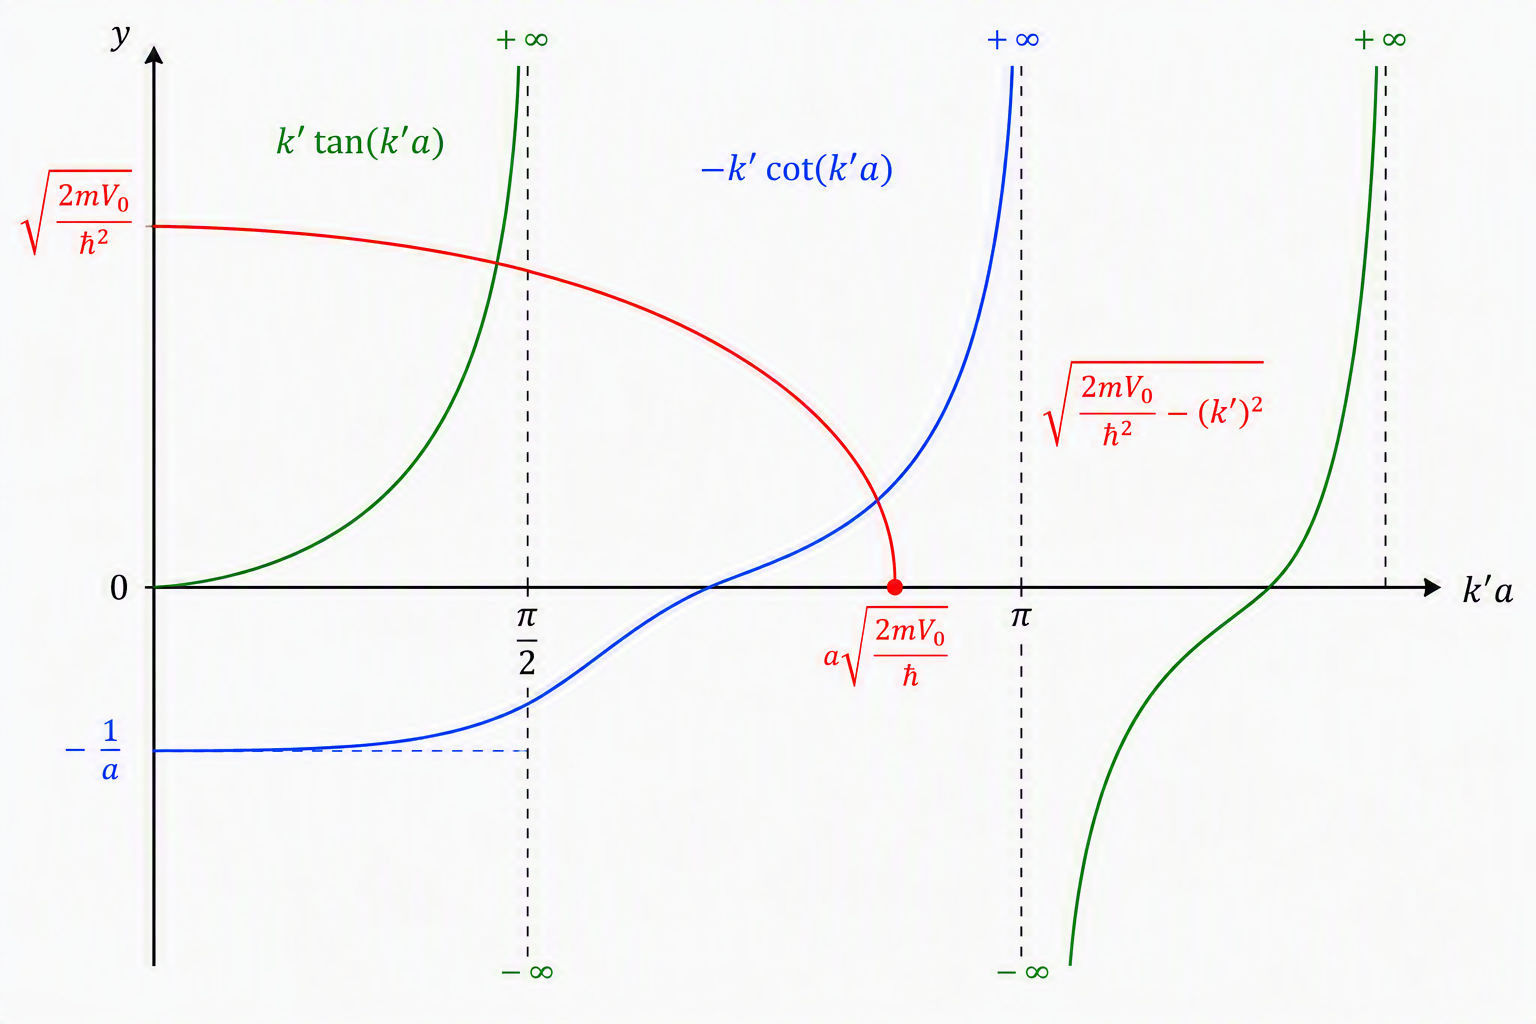
\includegraphics[width=\textwidth]{1d_finite_well_bound_states.png}
 \caption{Graphical solution of the even- and odd-parity finite-well
 bound-state equations. Intersections with the red curve determine the
 allowed bound-state energies.}
 \label{fig:finite-well-graphical-solution}
\end{figure}


Once an allowed $k'$ is found,
\begin{equation}
 E=-V_0+\frac{\hbar^2(k')^2}{2m}.
\end{equation}
Only finitely many intersections occur for a well of finite depth and width,
so a finite square well supports finitely many bound states.

Finally, note that in the limit of 
\begin{align}
    a\rightarrow0^+,~~~V_0\rightarrow+\infty,~~~2aV_0\rightarrow|D_0|
\end{align}
the square potential well discussed here reduces to the delta function potential studied in the last section. 

\subsection{Summary}
%\addcontentsline{toc}{chapter}{Summary}
\begin{itemize}
 \item Bound states are square-normalizable and decay at spatial infinity.
 \item One-dimensional bound-state energy levels are nondegenerate.
 \item The ground state has no nodes, and successive excited states acquire
       one additional node each.
 \item For an even potential, nondegenerate bound states have definite parity.
 \item Finite-well energies follow from separate even- and odd-parity
       transcendental equations.
\end{itemize}


\section{Scattering in one dimension (10/21)}

\referto{\tong~14.1}

\subsection{S-matrix formulation}



\appendix

% Disable the automatic page break before sections in the appendix
\RemoveFromHook{cmd/section/before}

\chapter{Homework 1 (due 9/4)}

\section{Franck-Hertz experiment}

In the Franck-Hertz experiment (see Fig. \ref{fig:franck-hertz} in lecture notes), the sharp drop of electric current through the vacuum tube at a voltage of 4.9 V corresponds to the absorption of electron energy by the mercury atoms in the vacuum tube, where the atomic energy level of mercury atoms go through a transition. Compute the wavelength of light associated with this atomic energy level transition, show that it is approximately 254 nm, as observed in optical emission of the same vacuum tube.

\section{Davisson-Germer experiment}

(1) \emph{Bragg's law}~~~Consider the diffraction of a wave by a lattice of atoms with a lattice constant of $d$ between layers. Derive the Bragg's law
\begin{align}\label{bragg law}
n\lambda=2d\cos\frac\theta2,~~~n=0,1,2,3,\cdots
\end{align}
for the diffraction pattern.

\begin{figure}
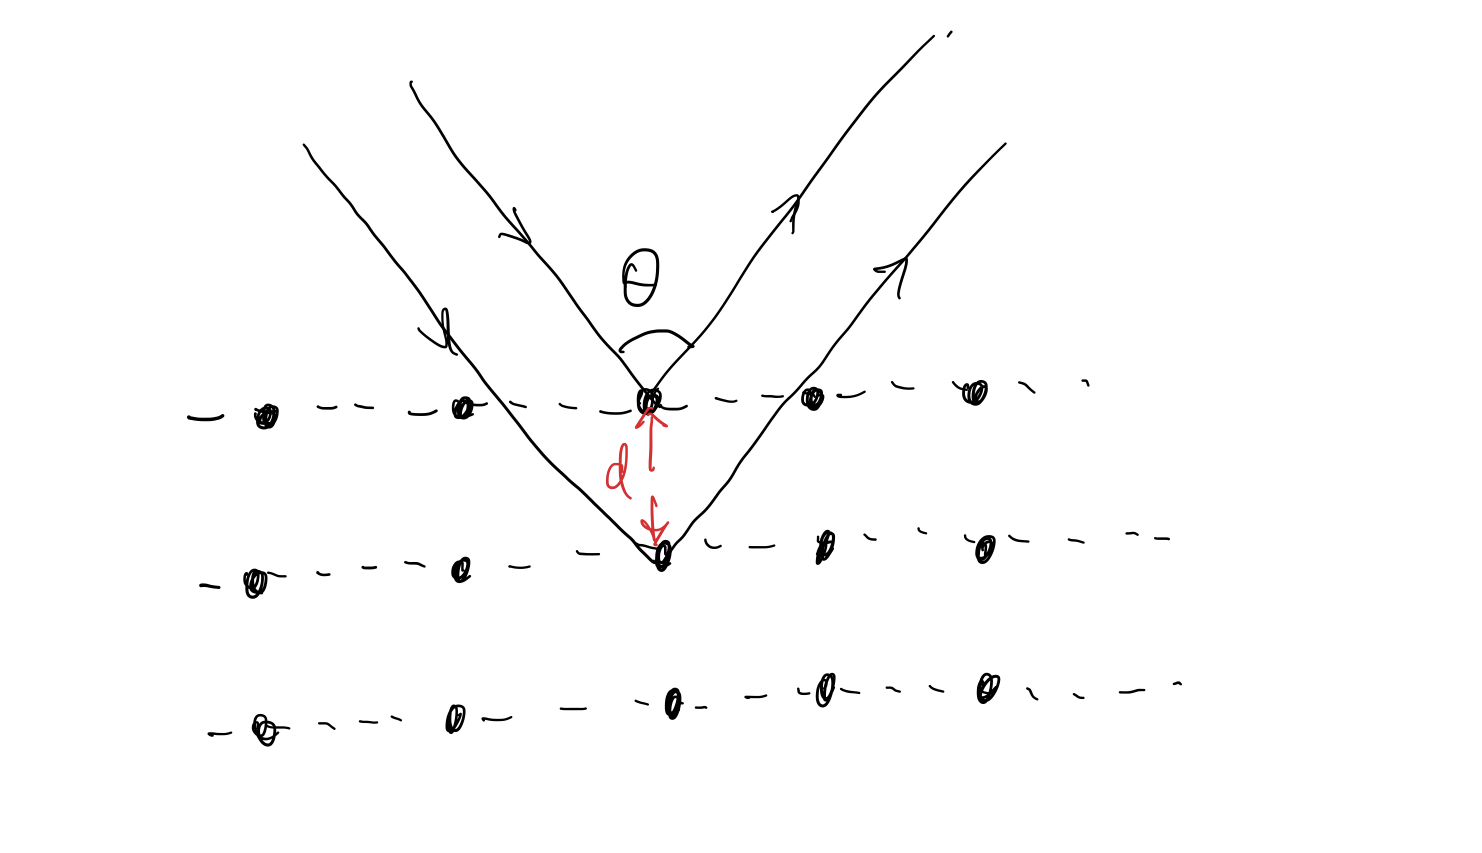
\includegraphics[width=0.9\columnwidth]{Bragg law.png}
\caption{Scattering of a wave by a lattice of atoms with a lattice constant $d$.}
\label{fig:bragg's law}
\end{figure}

(2) Consider the Davisson-Germer experiment illustrated in Fig. \ref{fig:davisson germer} of overleaf lecture notes. For $\theta=50^o$, $d=0.091$~nm for nickel crystals, and an electron beam accelerated by a $V=54$ volts voltage, show that it satisfies the Bragg's law with $n=1$.

In part (1) and (2), we have dealt with a simplified version of the actual Davisson-Germer experiment\cite{Davisson1927}, assuming the electron beam was scattered by a three-dimensional simple cubic lattice. Below we will seriously consider the actual situation of Davisson-Germer experiment in history, where an electron beam was scattered by the (111) surface of a nickel crystal in which Ni atoms form a face-centered cubic (FCC) lattice. In this case, we need to first derive the general Bragg condition for two-dimensional diffraction peaks and apply it to the setup of Davisson-Germer experiment. Below we carry out this calculation step by step.

(3) For electrons of energy $54$~eV in the Davisson-Germer experiment, their penetration depth into the nickel crystal is less than 1 nanometer, comparable to the FCC lattice constant $a=3.52$ \AA. This means as a zeroth order approximation, we can model the Davisson-Germer experiment as electrons scattered by the top layer of Ni atoms parallel to the crystal surface. In Davisson-Germer experiment the incident beam of electrons is perpendicular to the cleaved (111) surface of the nickel crystal. Can you draw the two-dimensional lattice formed on the (111) surface of a nickel crystal? Given the FCC lattice constant $a=3.52$ \AA in nickel cystals, what is the distance $\tilde a$ between two nearest Ni atoms on its (111) surface?

(4) For the two-dimensional (2d) plane parallel to the (111) surface, we can choose the following two orthonormal vectors as two basis vectors for the 2d plane:
\begin{align}
\hat e_1=(-1,1,0)/\sqrt2,~~~\hat e_2=(-1,-1,2)/\sqrt6,~~~\hat e_1\times\hat e_2=(1,1,1)/\sqrt3.
\end{align}
In this two-dimensional lattice on (111) surface, the periodic pattern of Ni atoms are described by two primitive vectors 
\begin{align}\label{hw1:primitive vectors}
\vec a_1=\tilde a \hat e_1,~~~\vec a_2=\tilde a\frac{-\hat e_1+\sqrt3\hat e_2}2.
\end{align}
where $\tilde a$ is the distance $\tilde a$ between two nearest Ni atoms on its (111) surface. They are called primitive vectors in the sense that any lattice site position $\vec R$ in the 2d lattice is a summation of integer multiples of $\vec a_i$
\begin{align}
\vec R=\sum_{j=1}^2m_j\vec a_j,~~~m_j\in\mbz.
\end{align}
One can also define \emph{reciprocal lattice primitive vectors} $\vec b_{1,2}$ by the following conditions
\begin{align}
\vec a_i\cdot\vec b_j=2\pi\delta_{i,j}
\end{align}
Note that $\vec b_{1,2}$ are both perpendicular to (1,1,1) as well. 

\textbf{For $\vec a_{1,2}$ defined in (\ref{hw1:primitive vectors}), express $\vec b_{1,2}$ using $\tilde a$ and $\hat e_{1,2}$.}\\

Most generally, the Bragg condition for diffraction peaks is given by
\begin{align}\label{bragg condition}
\sum_{\vec R}e^{\imth\vec q\cdot\vec R}\neq0\Longleftrightarrow\vec q\cdot\vec a_j=0\mod2\pi,~~~\forall~j=1,2.
\end{align}
where $\vec q$ is the in-plane component of electron momentum transfer before and after scattered by the nickel crystal:
\begin{align}\label{inplane mtm transfer}
\vec q\equiv(\vec k_\text{out}-\vec k_\text{in})-\frac{(1,1,1)}3(\vec k_\text{out}-\vec k_\text{in})\cdot(1,1,1).
\end{align}
In later lectures we will come back to (\ref{bragg condition}) when discussing Fourier transform as a change of basis (i.e. a unitary transformation). \textbf{From (\ref{bragg condition}), show that
\begin{align}\label{bragg peaks}
&\vec q=\sum_{j=1}^2n_j\vec b_j,~~~n_j\in\mbz
\end{align}}

(5) In the Davisson-Germer experiment, the incident momentum $\vec k_\text{in}$ is perpendicular to the (111) surface i.e. $\vec k_i=\frac{2\pi}{\lambda}(1,1,1)/\sqrt{3}$ where $\lambda$ is the wavelength of electrons with a kinetic energy of 54 eV. For elastic scatterings responsible for the diffraction pattern, we have 
\begin{align}\label{elastic scattering}
|\vec k_i|=|\vec k_f|=\frac{2\pi}{\lambda}
\end{align}
In the experimental setup of Fig. \ref{fig:davisson germer} (left), using results (\ref{inplane mtm transfer})-(\ref{bragg peaks}) of the previous part, derive the following Bragg's law for Davisson-Germer experiment:
\begin{align}\label{bragg cond:davisson germer}
\lambda\sqrt{n_1^2+n_1n_2+n_2^2}=\sqrt{\frac38}a\sin\theta,~~~n_{1,2}\in\mbz
\end{align}

Comment: specifically, if we choose $(n_1,n_2)=n(1,0)$ or $n(0,1)$ or $n(1,-1)$, Eq. (\ref{bragg cond:davisson germer}) reduces to the more familiar one
\begin{align}
n\lambda=d_{(111)}\sin\theta,~~~n\in\mbz,~~~d_{(111)}=a\sqrt{3/8}\approx2.16~\text{\AA}.
\end{align}

(6) Note that the in-plane momentum transfer $\vec q$ can be written as
\begin{align}
\vec q=|q|(\cos\phi\hat e_1+\sin\phi\hat e_2)
\end{align}
where $\phi$ is the azimuth angle in Fig. \ref{fig:davisson germer} of the lecture notes. Use relations (\ref{inplane mtm transfer})-(\ref{elastic scattering}) to explain the $\phi$-dependent peaks in the right panel of Fig. \ref{fig:davisson germer}.

(7) \textbf{Bonus} Can you qualitatively explain in Fig. \ref{fig:davisson germer} right panel, why are the peak heights at $\phi=\frac\pi2\mod2\pi/3$ are different from those at $\phi=\frac\pi6\mod2\pi/3$?

\section{Hilbert space $\mathbb{L}_\mathbb{V}$ of linear operators on $\mathbb{V}=\mathbb{C}^n$}

(1) Consider linear operators on complex vector space $\mathbb{V}=\mathbb{C}^n$, i.e. $n\times n$ complex matrices. Prove that they form a vector space, which we label as $\mathbb{L}_\mathbb{V}$. For the definition of a vector space, refer to Chapter 1.1 of \shankar.

(2) Prove that the following binary operation $(\cdot,\cdot)$ on $\mathbb{L}_\mathbb{V}\times \mathbb{L}_\mathbb{V}$ defined by
\begin{align}
(A,B)\equiv\text{tr}(A^\dagger B),~~~A,B\in\mathbb{L}_\mathbb{V}
\end{align}
is an inner product. For the definition of an inner product, refer to \shankar~1.2 or \nielsen~2.1.4. This is known as the Hilbert-Schmidt inner product on operators.

(3) Using the above Hilbert-Schmidt inner product, show that 3 Pauli matrices $\sigma_x,\sigma_y,\sigma_z$ defined below
\begin{align}
\sigma_x=\bpm0&1\\1&0\epm,~~\sigma_y=\bpm0&-\imth\\ \imth&0\epm,~~\sigma_z=\bpm1&0\\0&-1\epm
\end{align}
and the $2\times2$ identity matrix $\hat 1$ together can form a complete orthonormal basis for the vector space $\mathbb{L}_{\mathbb{C}^2}$ of all $2\times 2$ complex matrices.

(4) \textbf{Bonus} Prove the following \emph{completeness relation of Pauli matrices}:
\begin{align}
\sum_{i=x,y,z}(\sigma_i)_{a,b}(\sigma_i)_{c,d}=\vec\sigma_{a,b}\cdot\vec\sigma_{c,d}=2\delta_{a,d}\delta_{b,c}-\delta_{a,b}\delta_{c,d}
\end{align}

Hint: use the conclusion of part (3), i.e. any $2\times 2$ Hermitian matrix $\hat M$ can be written as
\begin{align}
\hat M=\frac{\text{Tr}(\hat M)}2\hat 1_{2\times2}+\sum_{a=x,y,z}\frac{\text{Tr}(\hat M\sigma_a)}2\sigma_a
\end{align}

\section{Compton shift}

\textbf{Bonus} Consider the Compton effect discussed in lecture notes (Fig. \ref{fig:compton}), where an $X$-ray photon was scattered by a stationary electron. Use energy and momentum conservations to derive the Compton shift formula:
\begin{align}
    \lambda^\prime-\lambda=\frac{h}{m_ec}(1-\cos\theta)
\end{align}
\chapter{Homework 2 (due 9/11)}


\subsection{Pauli matrices}

(1) Diagonalize the 3 Pauli matrices and find out their eigenvalues and eigenkets:
\begin{align}
\sigma_x=\bpm0&1\\1&0\epm,~~\sigma_y=\bpm0&-\imth\\ \imth&0\epm,~~\sigma_z=\bpm1&0\\0&-1\epm
\end{align}

(2) For an arbitrary function $f(\cdot)$ from complex numbers to complex numbers, if $\vec n$ is a normalized vector in three dimensions and $\theta$ is a real number, prove the following relation
\begin{align}
f(\theta\vec n\cdot\vec\sigma)=\frac{f(\theta)+f(-\theta)}2\hat 1+\frac{f(\theta)-f(-\theta)}2\vec n\cdot\vec\sigma
\end{align}
where $\vec\sigma=(\sigma_x,\sigma_y,\sigma_z)$ are three Pauli matrices.

Hint: a function $f(\hat M)$ of a matrix (operator) $\hat M$ can be defined by the Taylor expansion:
\begin{align}
f(\hat M)=\sum_{n=0}^\infty\frac{\hat M^n}{n!}\frac{\text{d}^{n}f}{\text{d}x^n}|_{x=0}
\end{align}



\subsection{Linear algebra}

(1) Use the Cauchy-Schwarz inequality to prove the triangle inequality
\begin{align}
|\dket{u}+\dket{v}|\leq|\dket{u}|+|\dket{v}|,~~~\forall~\dket{u},\dket{v}\in V
\end{align}

(2) A linear operator $\hat P$ is a projection operator (or a projector) if $\hat P^2=\hat P$. Prove that the eigenvalues of a projector are all either $0$ or $1$. 

(3) \textbf{Bonus} A projector has the following form:
\begin{align}
\hat P=\alpha\dket{1}\dbra{1}+\beta\dket{2}\dbra{2}
\end{align}
where $\dket{1}$ and $\dket{2}$ are two normalized vectors in the Hilbert space that are linearly independent. What conditions should coefficients $\alpha$ and $\beta$ satisfy in order for $\hat P$ defined above to be a projector (i.e. to satisfy $\hat P^2=\hat P$)?

%(4) Prove that a positive operator $\hat O$ satisfying 
%\begin{align}
%\expval{v|\hat O|v}\geq0,~~~\forall~\dket{v}\in\mathbb{V}
%\end{align}
%is necessarily Hermitian.

%Hint: any linear operator can be written as $O=H_1+\imth H_2$, where $H_{1,2}$ are two Hermitian operators.t

%(4) \textbf{ Bonus} Prove that a Hermitian linear operator $\hat O=\hat O^\dagger$ can be diagonalized, referring to how the spectral decomposition theorem is proved in Box 2.2 of \nielsen.


(4) Assume Hamiltonian $H$ commutes with two linear operators, $A_1$ and $A_2$, which do not commute with each other:
\begin{align}
[H,A_1]=[H,A_2]=0,~~~[A_1,A_2]\neq0
\end{align}
Show that the eigenstates of $H$ are in general degenerate. 

(5) Assume two observables $A_1$ and $A_2$ anticommutes with each other, i.e.
\begin{align}
    \{A_1,A_2\}=A_1A_2+A_2A_1=0
\end{align}
Show that for any eigenstate $\dket{\psi_1}$ of observable $A_1$ with a nonzero eigenvalue, its expectation value w.r.t. $A_2$ must vanish
\begin{align}
    \expval{\psi_1|A_2|\psi_1}=0
\end{align}
Comment: One such example is Pauli matrices $A_1=\sigma_x$ and $A_2=\sigma_y$. 


(5) \textbf{Bonus} For two linear operators satisfying $[\hat A,\hat B]=\alpha\hat 1$ where $\hat 1$ is the identity operator, prove the following identity:
\begin{align}
[\hat A,e^{\hat B}]=\alpha e^{\hat B}
\end{align}

Hint: first show that
\begin{align}
\hat f(x)=e^{-x \hat B}\hat Ae^{x\hat B}=\hat A+x\alpha\hat 1
\end{align}

\subsection{Consecutive measurements of incompatible operators}

Two consecutive projective measurements, for Pauli matrices $\hat \sigma_x$ and $\hat \sigma_z$ respectively, are carried out one after another on a quantum state of a single qubit (i.e. a Hilbert space $\mathbb{V}=\mathbb{C}^2$). In the first procedure, we first measured $\hat\sigma_x$ with an outcome $+1$ and probability $p(X=+1)$, and then measured $\hat\sigma_z$ with an outcome $+1$ with probability $p(Z=+1|X=+1)$. In the second procedure, we switched the order of the two measurements, i.e. we first measured $\hat\sigma_z$ with an outcome $+1$ and probability $p(Z=+1)$, and then measured $\hat\sigma_x$ with an outcome $+1$ with probability $p(X=+1|Z=+1)$. It is found that the probabilites do no depend on the order of the two incompatible measurements, i.e.
\begin{align}\label{hw3.1}
p(X=+1)=p(X=+1|Z=+1),~~~p(Z=+1|X=+1)=p(Z=+1)
\end{align}

(1) Find a single-qubit pure state $\dket{\psi}$ that satisfies the condition (\ref{hw3.1}). 

(2) If the quantum state is a single-qubit mixed state, it is generally described by a density matrix of the following form:
\begin{align}
\hat\rho=\frac{\hat 1+\vec r\cdot\vec\sigma}2,~~~\vec r=(x,y,z)\in\mathbb{R}^3,~~~|\vec r|\leq1.
\end{align}
Find those mixed states that satisfy the same condition (\ref{hw3.1}). 

\subsection{Quantum Zeno effect}

Consider a single qubit evolving under the following Hamiltonian:
\begin{align}
\hat H=-\mu_BB\hat\sigma_z
\end{align}
where $\mu_B=\hbar e/2m_e$ is the Bohr magneton. We define time $T$ as follows:
\begin{align}
T=\frac{\pi m_e}{eB}
\end{align}
Starting from the initial state
\begin{align}
\dket{\psi_0}=\dket{+}=\frac{\dket{\uparrow}+\dket{\downarrow}}{\sqrt2}
\end{align}
at time $t=0$, we evolve the system by time $T/n$, followed by a measurement of $\hat\sigma_x$, and then repeat the same 2-step (evolution by $\frac{T}{n}$ + $\hat\sigma_x$ measurement) procedure $n$ times. What is the probability at time $T$ (after $n$ such 2-step procedures) to produce the measurement outcome of $\sigma_x=+1$?
\chapter{Homework 3 (due 9/18)}


\subsection{Spin precession}

(1) For a unit vector $\vec n=(\sin\theta\cos\phi,\sin\theta\sin\phi,\cos\theta)$, diagonalize the matrix $\vec n\cdot\vec\sigma=\sum_{i=x,y,z}n_i\sigma_i$. Prove that it has two eigenvalues $\pm1$, and find out the two eigenvectors. 

(2) We denote $\dket{\vec n}$ as the eigenvector of $\vec n\cdot\vec\sigma$ with eigenvalue $+1$. Starting from time zero, the state vector $\dket{\psi(0)}\equiv\dket{\vec n}$ evolves under the following Hamiltonian:
\begin{align}
\hat H=-B\sigma_z
\end{align}
Prove that the following expectation value of $S_z=\hbar\sigma_z/2$ 
\begin{align}
\expval{S_z(t)}\equiv\expval{\psi(t)|S_z|\psi(t)}
\end{align}
does not change with time. 

(3) Compute the time-dependent expectation values of $S_x$ and $S_y$, and show that they oscillate with time. 

(4) Compute the transition probability that the state vector $\dket{\vec n}$ returns to itself after time $t$:
\begin{align}
P(\vec n\rightarrow\vec n:t)\equiv|\expval{\psi(t)|\psi(0)}|^2
\end{align}

\subsection{Neutrino oscillation}

Read the neutrino oscillation in \sakurai~2.1. Using the energy eigenvalues
\begin{align}
E_i=\sqrt{p^2c^+m_i^2c^4}\approx pc(1+\frac{m_i^2c^2}{2p^2})
\end{align}
prove the probability
\begin{align}
P(\nu_e\rightarrow\nu_e)=1-\sin^2(2\theta)\sin^2\big[\frac{(m_1^2-m_2^2)c^4t}{4E\hbar}\big],~~~E\approx pc.
\end{align}

\subsection{Propagator}

(1) Consider the following propagator for Hamiltonian $\hat H$:
\begin{align}
    G(i,f;t)\equiv-\imth\expval{f|e^{-\imth\hat Ht/\hbar}|i}
\end{align}
Show that its Fourier transform
\begin{align}
    G(i,f:\omega+\imth0^+)\equiv\lim_{\epsilon\rightarrow0^+}\int_0^\infty e^{\imth(\omega+\imth\epsilon)t}G(i,f:t)
\end{align}
is equal to
\begin{align}
    G(i,f:\omega+\imth0^+)=\expval{f|\frac{1}{\omega+\imth0^+-\hat H}|i}
\end{align}
where we have set $\hbar=1$. 

(2) \textbf{Bonus} Now consider a quantum particle in one dimension, by choosing $i,f$ to be position eigenstates $\dket{i}=\dket{x}$, $\dket{f}=\dket{y}$. Show that
\begin{align}
    G(x,y;t)=-\imth\sum_n\psi^\ast_n(x)\psi_n(y)e^{-\imth E_nt/\hbar}
\end{align}
where $E_n$ and $\psi_n(x)$ are the eigenvalues and eigenstates of Hamiltonian $\hat H$. 

(3) \textbf{Bonus} Show that the imaginary part of the frequency-domain propagator is given by
\begin{align}
    \Im G(x,x;\omega+\imth0^+)=-\pi\sum_n|\psi_n(x)|^2\delta(\omega-E_n/\hbar)
\end{align}
where $\delta(x)$ is a Dirac delta function. 

\subsection{2-qubit Hamiltonian}

Consider a closed quantum system consisting of two spin-$1/2$ particles $\{\vec S_i=\frac\hbar2\vec\sigma_i|i=1,2\}$, i.e. two qubits. The Hamiltonian of the system is given by the \emph{Heisenberg model}
\begin{align}\label{2-qubit heisenberg model}
\hat H=J\vec S_1\cdot\vec S_2=\sum_{a=x,y,z}J S_{1,a}\otimes S_{2,a}
\end{align}

(1) Using the matrix representation of Pauli matrices, show the commutation relation for each qubit:
\begin{align}
[S_{j,a},S_{j,b}]=\imth\hbar\epsilon_{abc}S_{j,c},~~~j=1,2;~~~a,b,c=x,y,z
\end{align}
where $\epsilon_{abc}$ is the Levi-Civita symbol. 

(2) Prove that each component of the total spin
\begin{align}
S^\text{tot}_a\equiv S_{1,a}\otimes\hat 1_2+\hat 1_1\otimes S_{2,a}
\end{align}
commutes with the Hamiltonian:
\begin{align}
[S^\text{tot}_a,\hat H]=0,~~~a=x,y,z.
\end{align}
The total spin of the system is defined as 
\begin{align}
S^2_\text{tot}=\vec S^\text{tot}\cdot\vec S^\text{tot}=\sum_aS^\text{tot}_aS^\text{tot}_a
\end{align}
Show that it commutes with both the Hamiltonian $\hat H$, and $S^\text{tot}_a,~a=x,y,z$.

(3) Show that if the Hamiltonian $\hat H$ commutes with another Hermitian operator $\hat O$ (known as a conserved quantity or a constant of motion), for any two eigenstates $\dket{\psi_1},\dket{\psi_2}$ of operator $\hat O$ with different eigenvalues $\lambda_1\neq\lambda_2$, the following matrix must vanish
\begin{align}
\expval{\psi_1|\hat H|\psi_2}=0
\end{align}
In other words, Hamiltonian $\hat H$ is a block diagnoal matrix in the eigenbasis of the conserved quantity $\hat O$. 

(4) Diagonalize the Hamiltonian $\hat H$ and find its energy levels. Find the simultaneous eigenstates of $\hat H$, $S^\text{tot}_z$ and $S^2_\text{tot}$, in the orthonormal basis of $\{\dket{\sigma_{1,z}=\pm1}\otimes\dket{\sigma_{2,z}=\pm1}\}$. Note: these 4 eigenstates can be properly chosen to form the \emph{Bell basis} of 2-qubit Hilbert space $\mathbb{C}^4$. (You are allowed to use computer programs, but please show your codes if you do so.)

(5) \textbf{Bonus} Can you explain the reason for the degenerate and non-degenerate energy levels, using what you have learnt from Problem 2.(4) in Homework 2?

\chapter{Homework 4 (due 9/25)}

\subsection{Bloch ball for single-qubit mixed states}

(1) Show that an arbitrary density matrix for a single-qubit mixed state can be written as
\begin{align}\label{Bloch sphere for mixed state}
\hat \rho=\frac{\hat 1+\vec r\cdot\hat{\vec\sigma}}2
\end{align}
where $\vec\sigma$ are 3 Pauli matrices, and $\vec r$ is a 3-dimensional vector such that $|\vec r|\leq1$. This vector $\vec r$ is known as the \emph{Bloch vector} for the state $\hat\rho$. 

Hint: a density matrix $\hat \rho$ is defined to satisfy two properties: $\hat \rho$ is positive (i.e. it can be diagnonalized and all eigenvalues are non-negative) and $\text{Tr}\rho=1$. 

(2) Show that a state $\rho$ is pure if and only if $|\vec r|=1$ i.e. $\vec r$ is a unit vector. 

Hint: a density matrix $\hat\rho$ is a pure state if and only if $\hat\rho^2=\hat\rho$.

(3) Consider the eigenstate $\dket{\vec r}$ of operator $\vec r\cdot\vec\sigma$ with eigenvalue $+1$, where $\vec r$ is a unit vector. Show that in this case, its density matrix $\rho=\dket{\vec r}\dbra{\vec r}$ is exactly given by Eq. (\ref{Bloch sphere for mixed state}) with $\vec r$ being a unit vector. This is known as the Bloch sphere. 

(4) Compute the von Neumann entropy $S(\rho)=-\trace\rho\log\rho$ for the mixed state (\ref{Bloch sphere for mixed state}). Plot it as a function of $|\vec r|$. 


\subsection{Entanglement entropy}

(1) If $\rho_1$ and $\rho_2$ are two density matrices, show that
\begin{align}\label{convex set:density matrix}
\hat\rho(x)\equiv x\hat\rho_1+(1-x)\hat\rho_2,~~~0\leq x\leq1.
\end{align}
is also a density matrix. 

(2) \textbf{ Bonus} Assume that $\hat\rho(x)$ in (\ref{convex set:density matrix}) is always invertible for any $0\leq x\leq1$, i.e. its inverse matrix $[\hat\rho(x)]^{-1}$ always exists. Prove that its von Neumann entropy is a concave function of $x$, i.e.
\begin{align}\label{concave:entropy}
\frac{\text{d}^2S(\hat\rho(x))}{\text{d}x^2}\leq0
\end{align}

(3) \textbf{ Bonus} Use the concave property (\ref{concave:entropy}) to prove the concavity of von Neumann entropy
\begin{align}
S(\sum_jp_j\hat\rho_j)\geq\sum_jp_jS(\hat\rho_j)
\end{align}
where $\{p_j\}$ is a probability distribution and $\{\hat\rho_j\}$ is a set of density matrices. 

Hint: for a concave function $f(x)$ satisfying $f^{\prime\prime}\leq0$, we always have $f(px_1+(1-p)x_2)\geq pf(x_1)+(1-p)f(x_2)$ for $0\leq p\leq 1$.

(4) Consider a pure state $\dket\psi_{AB}$ in a composite quantum system with Hilbert space $A\otimes B$. Show that for the reduced density matrices 
\begin{align}
\rho_A=\trace_B\dket{\psi_{AB}}\dbra{\psi_{AB}},~~~\rho_B=\trace_A\dket{\psi_{AB}}\dbra{\psi_{AB}}
\end{align}
they share the same von Neumann entropy
\begin{align}
S(\rho_A)=S(\rho_B)
\end{align}
Therefore either $S(\rho_A)$ or $S(\rho_B)$ can be defined as the entanglement entropy. 

(5) Consider a composite system of two qubits $A$ and $B$. Can you write down the generic form of a maximally entangled state $\dket{\psi_{AB}}$, satisfying that the reduced density matrix has a maximal entanglement entropy?

Hint: for a maximally entangled 2-qubit state, we must have
\begin{align}
\hat\rho_A=\hat\rho_B=\frac12\hat1.
\end{align}
so that $S(\rho_{A,B})=\log2$. 


(6) For a pure state in a composite system of 2 qubits $A$ and $B$:
\begin{align}
\dket{\psi_{AB}}=\alpha\dket{00}+\beta\dket{01}+\gamma\dket{10}+\delta\dket{11}
\end{align}
show that this state is (bipartite) entangled if and only if 
\begin{align}
\alpha\delta-\beta\gamma\neq0.
\end{align}

Hint: a pure state is (bipartite) entangled if and only if its bipartite entangled entropy is nonzero:
\begin{align}
S(\rho_A)=S(\rho_B)>0
\end{align}

(7) \textbf{Bonus} This problem is about \emph{tripartite entanglement}. Show that in a 3-qubit system, there are pure states that cannot be written in the following form:
\begin{align}
\dket{\psi}=\sum_{j=1}^2\lambda_{j}\dket{\alpha_j}_1\otimes\dket{\beta_j}_2\otimes\dket{\gamma_j}_3.
\end{align}
where $\{\alpha_j\},~\{\beta_j\},~\{\gamma_j\}$ are any complete basis for $\mathbb{C}^2$. Find one such state. 

\subsection{Entanglement negativity}

When we consider a mixed state $\rho_{AB}$ defined in a composite system $A\otimes B$, the entanglement entropy $S(\rho_A)$ should be replaced by the mutual information
\begin{align}\label{mutual information}
I(A:B)\equiv S(\rho_A)+S(\rho_B)-S(\rho_{AB})
\end{align}
Clearly it reduces to the entanglement entropy in the special case when $\rho_{AB}$ is a pure state.

In a generic mixed state, the mutual information (\ref{mutual information}) is incapable of distinguishing classical correlation betweem $A$ and $B$ from the quantum entanglement. To capture bipartite quantum entanglement in a mixed state $\rho_{AB}$, we need to introduce new entanglement measures. One such quantity is (logarithmic) entanglement negativity:
\begin{align}\label{log negativity}
    E_{\mathcal{N}}(\rho_{AB})\equiv\log||\rho_{AB}^{T_A}||_1
\end{align}
where $T_A$ denotes a partial transpose on subsystem $A$. 

The trace norm $||\cdot||_1$ for a density matrix $\rho$ is defined as
\begin{align}
    ||\rho||_1\equiv\text{Tr}\sqrt{\rho^\dagger\rho}=\sum_i|\lambda_i|
\end{align}
where $\{\lambda_i\}$ are the eigenvalues of density matrix $\rho$. 

Obviously the logarithmic negativity $E_{\mathcal{N}}$ vanishes if all eigenvalues of $\rho_{AB}^{T_A}$ are non-negative.

(1) Show that 
\begin{align}
    E_{\mathcal{N}}(\rho_{AB})=\log(1+2\sum_{\lambda_i<0}|\lambda_i|)
\end{align}
where $\{\lambda_i\}$ are all eigenvalues of matrix $\rho_{AB}^{T_A}$. 

(2) Now consider a composite system of two qubits, one qubit in $A$ and one qubit in $B$. Show that for the Bell state $\dket{Bell_0}$ in this composite system, the logarithmic negativity is $\log2$. 

(3) \textbf{Bonus} Next consider a mixed state, which is the equilibrium density matrix at inverse temperature $\beta=J/k_BT$ ($J$ is a constant of the dimension of energy)
\begin{align}
    \rho_{AB}\propto e^{-\beta Z_A\otimes Z_B}
\end{align}
where $\hat Z=\bpm1&0\\0&-1\epm$ is the 3rd Pauli matrix. Show that its logarithmic negativity (\ref{log negativity}) vanishes, while the mutual information (\ref{mutual information}) is nonzero. Plot its mutual information as a function of $\beta>0$. 

 


\chapter{Homework 5 (due 10/2)}


\subsection{Revisiting the quantum Zeno effect}

We will now revisit the quantum Zeno effect in the lens of generalized measurements. Consider an initial state of a single qubit 
\begin{align}\label{quantum zeno:initial state}
\hat{\rho}_0=\dket{+}\dbra{+},~~~\dket{+}=\frac{\dket{0}+\dket{1}}{\sqrt2}
\end{align}
evolving under the following Hamiltonian
\begin{align}
\hat H=-\mu_BB\hat Z,~~~T=\frac{\pi m_e}{eB}
\end{align}
where $\mu_B=\hbar e/2m_e$ is the Bohr magneton. After a small period $\Delta t=T/n$ of unitary time evolution, we carry out a projective measurement on Pauli matrix $\hat X$. Recall that while $\dket{0},\dket{1}$ are eigenstates of Pauli $\hat Z$ operator, $\dket{\pm}$ are eigenstates of $\hat X$.  

(1) As we have learnt in the lecture, the 2-step procedure, of unitary time evolution for $\Delta t=T/n$ followed by a projective measurement on $\hat X$, can be described by a generalized measurement. Compute the measurement operators $\{\hat M_m|m=\pm\}$ as $2\times2$ matrices, and show that they satisfy the completeness relation
\begin{align}
\sum_{m=\pm}\hat M^\dagger_m\hat M_m=\hat1. 
\end{align}

(2) In the generalized measurement discussed above, if we do not know the measurement outcomes, the density matrix after the measurement is given by the action of a quantum channel $\mathcal{E}$, which is characterized by measurement operators $\{\hat M_m\}$:
\begin{align}\label{quantum zeno:quantum channel}
\mathcal{E}[\hat\rho]\equiv\sum_m\hat M_m\hat\rho\hat M_m^\dagger
\end{align}
We have previously learnt that any single-qubit density matrix can be expressed in terms of the Bloch ball:
\begin{align}
\hat\rho=\frac{\hat 1+\vec r\cdot\vec\sigma}2,~~~|\vec r|\leq1.
\end{align}
How does the vector $\vec r$ transform under the quantum channel (\ref{quantum zeno:quantum channel})?

(3) In the discussion of quantum Zeno effect, such a generalized measurement (without knowing measurement outcomes) was performed $n$ times. Starting from the initial density matrix $\hat\rho_0$ in (\ref{quantum zeno:initial state}), what is the final density matrix $\mathcal{E}^n[\rho_0]$ after $n$ such operation? 

Hint: use the results of part (2). 


(4) Using the above results, compute the probability at time $T$ (after $n$ such 2-step procedures) to produce the measurement outcome of $\sigma_x=+1$. 

Comment: recall that we have obtained this probability in HW2. You should compare your results here to HW2.  

\subsection{Measurements}

(1) \textbf{Bonus: distinguishing states by POVM measurements} \nielsen~Exercise 2.64. 

(2) Let $\dket{\psi=a\dket{0}+b\dket{1}}$ be any single-qubit quantum state. Suppose we receive one of the four states $\dket\psi,~\hat X\dket\psi,~\hat Y\dket\psi,~\hat Z\dket\psi$ with equal prior probabilities of 1/4, where $(\hat X,\hat Y,\hat Z)$ are the three Pauli matrices. This is known as Pauli-twirling. Show that the density matrix received by us is exactly $\hat\rho=\frac12\hat1$. 

Comment: for such a single-qubit mixed state with $\hat\rho=\frac12\hat1$, the outcome for any projective measurement $\hat P$ has a probability of one half, thus the received state contains no information at all about the identity of $\dket\psi$. This is Problem 4 in Chapter 16 exercises of \tong. 



\subsection{Quantum channels}

(1) \textbf{Bonus} Consider an open quantum system $A$ interacting with its environment $B$. In the lectures, we have shown that for an initial state of $\rho_A\otimes\dket{0}\dbra{0}_B$ where $\dket{0}$ is a pure state in $B$, the time evolution for system $A$ is given by a quantum channel $\varepsilon$, which is specified by a set of Kraus operators $\{\hat M_k\}$ satisfying the completeness relation 
\begin{align}
\sum_k\hat M_k^\dagger\hat M_k=\hat 1_A.
\end{align}
Show that this is still true if we consider the initial state to be a product state $\rho_A\otimes\rho_B$, where $\rho_B$ is an arbitrary density matrix in $B$.

Hint: you will need to find the set of Kraus operators satisfying the completeness relation in this case. It is convenient to work in the eigenbasis of $\rho_B$.  
 
(2) \nielsen~Exercise 8.15

%(3) \nielsen~Exercise 8.18

(3) \textbf{Bonus: generalized depolarizing channel} \nielsen~Exercise 8.19

%(5) \nielsen~Exercise 8.28




\subsection{The master equation}

\subsubsection{Phase damping}

Time evolution of a single-qubit open system under the phase damping quantum channel $\varepsilon_z$ is given by:
\begin{align}
\hat\rho=\bpm\rho_{11}&\rho_{12}\\ \rho_{21}&\rho_{22}\epm\rightarrow\varepsilon_z[\hat\rho]=(1-p)\hat\rho+p\hat Z\hat\rho \hat Z=\bpm\rho_{11}&(1-2p)\rho_{12}\\ (1-2p)\rho_{21}&\rho_{22}\epm
\end{align}
where $p$ is the probability of error. For the time evolution by a small time $\Delta t$, the error probability is given by
\begin{align}
2p=\Gamma\Delta t
\end{align}
where $\Gamma$ is the rate of error. 

(1) Derive the differential equation 
\begin{align}
\frac{\text{d}\rho}{\text{d}t}=\lim_{\Delta t\rightarrow0^+}\frac{\varepsilon_z[\rho]-\rho(t=0)}{\Delta t}
\end{align}
and solve it. Obtain the form of $\rho(t)$ for a given initial state $\hat\rho(t=0)=\bpm\rho_{11}&\rho_{12}\\ \rho_{21}&\rho_{22}\epm$. 

(2) Write the differential equation in part (1) into the form of a master equation. Find the Hamiltonian $\hat H$ and the Lindblad operators $\{\hat L_k\}$ in the master equation. 


\subsubsection{Amplitude damping}

(1) Solve the following master equation for a 1-qubit density matrix $\rho(t)$, with a single Lindblad operator $L=\sqrt{\lambda}\sigma_-\equiv\sqrt{\lambda}(\hat X-\imth\hat Y)/2=\sqrt{\lambda}\bpm0&0\\1&0\epm$:
\begin{align}
\frac{\text{d}\rho}{\text{d}t}=\lambda\sigma_-\rho\sigma_+-\frac\lambda2\{\rho,\sigma_+\sigma_-\}
\end{align}
where $\sigma_+=(\hat X+\imth\hat Y)/2=\bpm0&1\\0&0\epm$. Express $\rho(t)$ as a function of the initial density matrix
\begin{align}\label{amplitude damping:initial state}
\rho(t=0)=\bpm\rho_{11}&\rho_{12}\\ \rho_{21}&\rho_{22}\epm
\end{align}

Comment: this master equation describes the amplitude damping of a 1-qubit system. 

(2) Consider the time evolution of a 1-qubit system by an amplitude-damping quantum channel $\varepsilon_p$ with the following set of Kraus operators:
\begin{align}
\hat M_0=\bpm\sqrt{1-p}&0\\0&1\epm,~~~\hat M_1=\bpm0&0\\ \sqrt p&0\epm
\end{align}
For the same initial state (\ref{amplitude damping:initial state}), obtain the final density matrix $\rho(p)=\varepsilon_p[\rho(t=0)]$ after the action of the quantum channel, as a function of the amplitude-damping probability $p$. Compare it with the previous problem, and obtain the relation between $p$ in this problem, and $t$ in the previous problem. 

\subsubsection{Amplitude + phase dampings}

\textbf{Bonus} \nielsen~Exercise 8.30. There is a typo in \nielsen~for this problem: you need to show that $T_2=2T_1$ for amplitude damping only, and $T_2\leq 2T_1$ for both amplitude and phase dampings. 

\chapter{Homework 6 (Due 10/14)}

\subsection{(Bonus) Position and momentum operators on a discrete periodic chain}

During the lecture, we showed that the position-space basis $\{\dket{x}\}$ and momentum-space basis $\{\dket{p}\}$ in the continuum can be approached as the limit of a one-dimensional periodic ring of $L$ lattice sites $\{\dket{n}\equiv\dket{n+L}|1\leq n\leq L\}$, where two neighboring sites are separated by a lattice constant $a$. The unitary translation operator (it's easy to check $\hat T_x^\dagger\hat T_x=\hat1$)
\begin{align}\label{momentum:finite L}
\hat T_x=\sum_{n=1}^{L}\dket{(n\mod L)+1}\dbra{n}=e^{-\imth a\hat p/\hbar}
\end{align}
allows us to define the unitary momentum operator $\hat p$, and the position operator is given by
\begin{align}\label{position:finite L}
\hat x=\sum_{n=1}^{L}(n-\frac{L}2)a\dket{n}\dbra{n}
\end{align}
where $a$ labels the lattice constant. In lectures we claimed that in the simultaneous limits of $a\rightarrow0^+$ and $La\rightarrow\infty$, they correspond to the position and momentum operators in the continuum. In this problem, we consider them in a finite chain for a finite positive integer $L$. 

(1) \textbf{Bonus} Find all eigenvalues and their associated eigenstates of the translation operator $\hat T_x$ for a finite $L\in\mbz_+$.

Hint: there should be $L$ eigenstates for a $L\times L$ unitary operator. These are also eigenstates of momentum operator $\hat p$. 

%(2) Can you write down the matrix representation of the momentum operator $\hat p$ in the eigenbasis of translation operator $\hat T_x$?

%Hint: it should be a diagonal matrix since $\hat T_x=e^{-\imth a\hat p/\hbar}$. There is in fact an ambiguity in choosing the eigenvalues of $\hat p$ operator in (\ref{momentum:finite L}):
%\begin{align}
%p\simeq p+\frac{2\pi\hbar}{a}
%\end{align}
%but we can always choose the $\hat p$ eigenvalues to be in the following range to fix the ambiguity:
%\begin{align}
%-\frac{\pi\hbar}{a}\leq p<\frac{\pi\hbar}{a}
%\end{align}


(2) \textbf{Bonus} In lectures, we used the fact that $[\hat x,\hat T_x]=a\hat T_x$ to derive the commutation relation $[\hat x,\hat p]=\imth\hbar\hat1$. But we know that in a finite-dimensional Hilbert space, it is impossible for the commutator of two linear operators to be a nonzero constant matrix. Here we will investigate what really happens in a finite-dimensional space, which is $\mathbb{C}^L$ here. 

Compute the commutator $[\hat x,\hat T_x]$ of the position and translation operators defined in (\ref{position:finite L}) and (\ref{momentum:finite L}), in the complete orthonormal basis of $\{\dket{n}\}$. Show that it is almost the same as $a\hat T_x$, except for one matrix element. 


(3) \textbf{Bonus} For an arbitrary momentum eigenstate (you can choose any one of the $L$ eigenstates of $\hat T_x$), compute the variance of the position operator:
\begin{align}
(\Delta x)^2\equiv\expval{\hat x^2}-\expval{\hat x}^2
\end{align}
How does the variance increase with $L$ in the limit of $L\rightarrow\infty$?

\subsection{Dirac delta function}

(1) In lectures we learnt that the Dirac delta function is given by
\begin{align}
\delta(x)=\frac1{{2\pi}}\int\text{d}p~e^{\imth px}
\end{align}
However, this integral does not converge since the integrand $e^{\imth px}$ does not vanish at infinity. To regulate this integral, and to define Dirac delta function more rigorously, we define
\begin{align}
\delta(x)=\lim_{\lambda\rightarrow0^+}\int\frac{\text{d}p}{{2\pi}}e^{\imth px-\lambda p^2}
\end{align}
Carry out this integral to show that
\begin{align}\label{dirac delta:def}
\delta(x)=\lim_{\lambda\rightarrow0^+}\frac{e^{-x^2/4\lambda}}{\sqrt{4\pi\lambda}}
\end{align}

(2) Show that the above definition (\ref{dirac delta:def}) satisfies the properties of Dirac delta functions:
\begin{align}\label{dirac delta:parity}
&\delta(x)=\delta(-x),\\
&\delta(x\neq0)=0,\\
&\int\text{d}x~\delta(x)=1.\label{dirac delta:integral}
\end{align}

(3) Prove the following property of the delta function:
\begin{align}
\delta(ax)=\delta(x)/|a|
\end{align}

Hint: consider the property (\ref{dirac delta:integral}) of Dirac delta functions.  

(4) Prove another property of the delta function:
\begin{align}
\delta\big[f(x)\big]=\sum_i\frac{\delta(x-x_i)}{|\text{d}f/\text{d}x|_{x=x_i}}
\end{align}
where $x_i$ are the zeros of $f(x)$.

%Hint: Where does $\delta\big[f(x)\big]$ blow up? Expand $f(x)$ near such points in a Taylor series, keeping the first nonzero term. 


\subsection{Inversion symmetry in one dimension}

(1) For a one-dimensional quantum mechanics problem, consider the following unitary operator $\hat U$:
\begin{align}
\hat U=\int\text{d}x\dket{-x}\dbra{x}
\end{align}
Show that $\hat U$ is a unitary operator first. 

(2) How does operator $\hat U$ act on the momentum-space basis? Using Fourier transform to show that
\begin{align}
\hat U\dket{p}=\dket{-p}
\end{align}
$\hat U$ is known as the inversion symmetry operator. 

(3) Consider a bound state $\dket{\psi}$, which is also an eigenstate of a Hamiltonian
\begin{align}\label{ham:1d particle}
\hat H=\frac{\hat p^2}{2m}+V(\hat x)
\end{align}
satisfying $V(x)=V(-x)$. Show that 
\begin{align}
\expval{\psi|\hat x|\psi}=\expval{\psi|\hat p|\psi}=0
\end{align}

\subsection{Double delta function potential}

Because the inversion symmetry operator $\hat U$ commutes with the Hamiltonian, each energy eigenstate must also be an eigenstate of inversion operator $\hat U$. Consider the Hamiltonian (\ref{ham:1d particle}) with the following attractive potential
\begin{align}
V(x)=-V_0~\delta(x-x_0)-V_0~\delta(x+x_0)
\end{align}
where both $V_0$ and $x_0$ are positive constants. 

(1) Write down the form of the bound state wavefunction in the three regions:

\[
  (i)~x<-x_0, 
  \qquad
  (ii)~-x_0<x<x_0 
  \qquad (iii)~x>x_0
\]

(2) Write down the boundary condition equations at $x=\pm x_0$, to continuously connect the wavefunctions of the 3 regions. 

(3) Solve for the wavefunction of an energy eigenstate with a negative energy $E<0$. What is the inversion eigenvalue of this state?

Hint: recall that the energies of bound states are discrete. It won't be surprising if your results depend on the energy $E$ and parameters $V_0,x_0$.
\chapter{Homework 7 (due 10/28)}

\subsection{(Bonus) Lippmann-Schwinger equation}

In this problem, we delve into the derivation of Lippmann-Schwinger equation, which was briefly mentioned in our lectures. Consider a Hamiltonian 
\begin{align}
\hat H=\hat H_0+\hat V
\end{align}
where $\hat H_0$ is the non-interacting Hamiltonian which is exactly solvable, e.g. the free particle Hamiltonian $\hat p^2/2m$ in lectures. $\hat V$ represents an interaction term, e.g. the potential term $V(\hat x)$ for a quantum particle in free space, whose presence makes the full Hamiltonian $\hat H$ hard to solve. 

Next we assume that $\hat H$ and $\hat H_0$ have the same energy spectrum. This is exactly the case for a localized potential
\begin{align}
\lim_{|x|\rightarrow\infty}V(x)=0.
\end{align}
that we have discussed in lectures: it is obvious from the asymptotic behavior of the Schrodinger equation at $|x|\rightarrow\infty$. 

Now we label the orthonormal diagonal basis of non-interacting Hamiltonian $\hat H_0$ to be $\{\dket{a}\}$, satisfying
\begin{align}
\hat H_0\dket{a}=E_a\dket{a},~~~\expval{a|b}=\delta_{a,b}.
\end{align}
We further label the eigenstate of full Hamiltonian $\hat H$ with energy $E_a$ as $\dket{\psi^\pm_{a}}$, satisfying the stationary Schrodinger equation
\begin{align}
\hat H\dket{\psi^\pm_a}=(E_a\pm\imth\epsilon)\dket{\psi^\pm_a}
\end{align}
where $\epsilon\rightarrow0^+$ is an infinitely small positive number. 

(1) \textbf{Bonus} Show that 
\begin{align}
\dket{\psi^\pm_a}=\alpha\dket{a}+(E_a-\hat H_0\pm\imth\epsilon)^{-1}\hat V\dket{\psi^\pm_a}
\end{align}
where $\alpha$ is a complex coefficient.

Comment: we can always absorb the coefficient $\alpha$ into the un-normalized eigenstate $\dket{\psi^\pm_a}$, which leads to the familiar form of Lippmann-Schwinger equation:
\begin{align}
\dket{\psi^\pm_a}=\dket{a}+\frac1{E_a-\hat H_0\pm\imth\epsilon}\hat V\dket{\psi^\pm_a}
\end{align}
But it is sometimes important to keep the coefficient $\alpha$ in mind, as we will see in the next problem when we are dealing with piecewise continuous wavefunctions.\\

(2) \textbf{Bonus} Show that $\{\dket{\psi^+_a}\}$ forms another set of complete orthonormal basis of the Hilbert space. In other words, show that
\begin{align}
\expval{\psi^+_a|\psi^+_b}=\delta_{a,b}=\expval{a|b}
\end{align}

Comment: we need to use the Gellmann-Low theorem for this problem, which we mentioend during lectures. Similarly one can show that $\{\dket{\psi^-_a}\}$ is also a set of complete orthonormal basis. 

\subsection{(Bonus) Solving Lippmann-Schwinger eq. for a delta function potential}

Next, we will use the Lippmann-Schwinger equation to solve the eigenstate wavefunctions for scattering states with a delta function potential:
\begin{align}
\hat H=\hat H_0+\hat V,~~~\hat H_0=\frac{\hat p^2}{2m},~~~\hat V=V(\hat x)
\end{align}
Recall the Lippmann-Schwinger equation:
\begin{align}\label{hw7:lippmann-schwinger eq}
\psi^{\pm}_k(x)=\alpha\expval{x|k}+\int\text{d}yG_0^{\pm}(E|x,y)V(y)\psi^{\pm}_k(y)
\end{align}
where $\alpha$ is an arbitrary coefficient to be determined, and $\dket{k}$ is a plane wave 
\begin{align}
\expval{x|k}=\frac1{\sqrt{2\pi}}e^{\imth kx}
\end{align}
with wavevector $k=\sqrt{2mE}/\hbar>0$, with a positive energy $E>0$ for the free particle Hamiltonian $\hat H_0$. The retarded ($G^+$) and advanced ($G^-$) Green's functions are defined as 
\begin{align}\label{hw7:Green's function}
G_0^{\pm}(E|x,y)=\int\text{d}k\expval{x|k}\frac{1}{E-\hbar^2k^2/2m\pm\imth\epsilon}\expval{k|y}=\int\frac{\text{d}k}{2\pi}\frac{e^{\imth k(x-y)}}{E-\hbar^2k^2/2m\pm\imth\epsilon}
\end{align}
where $\epsilon\rightarrow0^+$ is an infinitely small positive number. 

(1) \textbf{Bonus} Show the following relation holds for an arbitrary potential $V(\hat x)$
\begin{align}
\big[\psi^+_k(x)\big]^\ast=\psi^-_{-k}(x)
\end{align}
using the Lippmann-Schwinger equation (\ref{hw7:lippmann-schwinger eq}). This relation is a consequence of the time reversal symmetry $\hat H^\ast=\hat H$.

(2) \textbf{Bonus} Using the contour integral in complex analysis, compute the retarded Green's function $G_0^+(E|x,y)$ in (\ref{hw7:Green's function}). Explain why it corresponds to an outgoing wave. 

Hint: it should have different behaviors in $x<y$ and $x>y$ regions. 

(3) \textbf{Bonus} Similarly compute the advanced Green's function $G_0^-(E|x,y)$ in (\ref{hw7:Green's function}). Explain why it corresponds to an incoming wave. 

(4) \textbf{Bonus} Now we turn to the delta function potential $V(x)=V_0\delta(x)$. We will focus on only the outgoing states $\dket{\psi^+_k}$. Write down the Lippmann-Schwinger equation (\ref{hw7:lippmann-schwinger eq}) for $x>0$ and $x<0$ separately. Note that the coefficient $\alpha$ can be different for the two regions. Solve the Lippmann-Schwinger equation to obtain the transmission and reflection coefficents $t$ and $r$. They should recover the exact solution we derived in lectures. 

\subsection{S matrix and the phase shift}

In lectures we have mentioned that the $S$ matrix defined as the change of basis between two sets of complete orthonormal basis $\{\dket{\psi^+_a}\}$ and $\{\dket{\psi_a^-}\}$ (see problem 1.(2)~)
\begin{align}
S_{a,b}=\expval{\psi_a^-|\psi_b^+}=\expval{a|U_I(+\infty,-\infty)|b}
\end{align}
is a unitary matrix, satisfying $\hat S^\dagger\hat S=\hat 1$. A unitary matrix can always be diagonalized, and its eigenvalues are phase factors $e^{2\imth\delta}$ known as phase shifts in scattering problems. We will learn more about the phase shift in this problem. 

In our lectures, we have derived the asymptotic form of exact eigenstates for an arbitrary localized potential $V(x)$ satisfying $\lim_{|x|\rightarrow\infty}V(x)=0$:
\begin{align}
\psi^+_k(x)=\begin{cases}
    t e^{\imth kx},~~~&x\rightarrow+\infty,\\
    e^{\imth kx}+re^{-\imth kx},~~~&x\rightarrow-\infty.
\end{cases}\\
\psi^+_{-k}(x)=\begin{cases}
    e^{-\imth kx}+r^\prime e^{\imth kx},~~~&x\rightarrow+\infty,\\
    t^\prime e^{-\imth kx},~~~&x\rightarrow-\infty.
\end{cases}
\end{align}
and 
\begin{align}
\psi^-_k(x)=\big[\psi^+_{-k}(x)\big]^\ast,~~~\psi^-_{-k}(x)=\big[\psi^+_{k}(x)\big]^\ast
\end{align}

(1) Using the continuity of probability flux, show that
\begin{align}\label{hw7:continuity}
|t|^2+|r|^2=1=|t^\prime|^2+|r^\prime|^2.
\end{align}

(2) Using the fact that $(t\psi^+_{-k}-r^\prime\psi_k^+)^\ast\propto\psi_k^+$ and relation (\ref{hw7:continuity}), show that
\begin{align}
t^\prime=t,~~~r^\prime=-r^\ast t/t^\ast.
\end{align}

(3) Using the relations proved in parts (1) and (2), show that 
\begin{align}
\expval{\psi_k^+|\psi^+_{-k}}=\expval{\psi_k^-|\psi^-_{-k}}=0.
\end{align}

Comment: this verifies that either $\{\dket{\psi_k^+},\dket{\psi_{-k}^+}\}$ or $\{\dket{\psi_k^-},\dket{\psi_{-k}^-}\}$ forms a complete orthogonal basis of the Hilbert space. 

(4) \textbf{Bonus} In the subspace with energy $E=\hbar^2k^2/2m>0$, the $\hat S$ matrix is given by
\begin{align}
\hat S(k)=\bpm\expval{\psi^-_{k}|\psi^+_{k}}&\expval{\psi^-_{k}|\psi^+_{-k}}\\ \expval{\psi^-_{-k}|\psi^+_{k}}&\expval{\psi^-_{-k}|\psi^+_{-k}}\epm
\end{align}
Diagonalize it to obtain its eigenvalues $e^{2\imth\delta_+}$ and $e^{2\imth\delta_-}$ as a function of $r$ and $t$. 

Hint: since $|t|^2+|r|^2=1$ we can parameterize them as
\begin{align}
t=\cos\theta e^{\imth\phi_t},~~~r=\sin\theta e^{\imth\phi_r},~~~0\leq\theta\leq\pi/2.
\end{align}

Comment: the diagonal basis of $\hat S(k)$ are inversion eigenstates with inversion eigenvalue $+1$ and $-1$ respectively, if the potential is inversion symmetric i.e. $V(-x)=V(x)$. 

\subsection{Tunneling through a finite potential barrier}

Consider a finite potential barrier
\begin{align}
V(x)=\begin{cases}
    0,~~~&|x|>a/2,\\
    U>0,~~~&|x|<a/2.
\end{cases}
\end{align}
where $a>0$ is the width of the potential barrier. 

(1) Consider an eigenstate, the in $\dket{\psi_k^+}$ with energy $0<E<U$. Write down the form of its eigenstate wavefunction $\psi_k^+(x)$, without computing the coefficients. 

(2) Write down the boundary conditions satisfied by $\psi_k^+(x)$ at $x=\pm a/2$.

(3) Obtain the reflection and transmission coefficients $r$ and $t$ as functions of $E,U,a$. 

(4) Show that in the low energy limit of 
\begin{align}
U-E\gg\frac{\hbar^2}{ma^2}
\end{align}
the transmission probability decays exponentially with $\sqrt{U-E}$
\begin{align}
T\equiv|t|^2\sim e^{-C\sqrt{U-E}}
\end{align}
Compute the coefficient $C$. 

(5) Now we consider $U<0$ case, i.e. a finite potential well which we discussed in details in our lectures. In this case, the even-parity bound state solution is determined by the following equation
\begin{align}
    k'\tan(k'a/2)=\sqrt{\frac{2m|U|}{\hbar^2}-(k')^2},~~~E=\frac{(\hbar k')^2}{2m}-|U|<0.
\end{align}
Show that in the limits of
\begin{align}
    a\rightarrow0^+,~~~|U|\rightarrow\infty,~~~a|U|=|D_0|=\text{const.}
\end{align}
the finite potential well is reduced to an attractive delta function $V(x)=-|D_0|\delta(x)$, and show the bound state energy is given by
\begin{align}
    E=-\frac{m|D_0|^2}{2\hbar^2}
\end{align}

\subsection{A step potential}

Consider the following step potential 
\begin{align}
V(x)=\begin{cases}
    0,~~~&x<0,\\
    U>0,~~~&x>0
\end{cases}
\end{align}

(1) Compute the wavefunction for an eigenstate with energy $E>U$.

(2) Compute the wavefunction for an eigenstate with energy $0<E<U$. 
\chapter{Homework 8 (due 11/4)}

\subsection{The simple harmonic oscillator}

(1) When we learnt about Heisenberg's uncertainty relation, we know that the equality $\Delta x\Delta p=\hbar/2$ holds when the following two conditions hold simultaneously:
\begin{align}\label{hw8:cond 1}
&(\Delta\hat x+C\Delta\hat p)\dket{\psi}=0,\\
&\expval{\psi|\{\Delta\hat x,\Delta\hat p\}|\psi}=0\label{hw8:cond 2}
\end{align}
where $C$ is a constant, and 
\begin{align}
\Delta\hat x\equiv\hat x-\expval{\hat x},~~~\Delta\hat p\equiv\hat p-\expval{\hat p}.
\end{align}
Using the fact that $\Delta\hat x$ and $\Delta p$ are both Hermitian operators, show that the constant $C$ must be an imaginary number (e.g. we can choose $C=\imth R^2/\hbar$), and the two conditions (\ref{hw8:cond 1})-(\ref{hw8:cond 2}) turn out to be just one condition
\begin{align}\label{hw8:cond 3}
(\Delta\hat x+\frac{\imth R^2}{\hbar}\Delta\hat p)\dket{\psi}=0
\end{align}
Here $R$ is a constant length scale. 

(2) Following our lecture discussions, the ground state $\dket0$ of simple harmonic oscillator Hamiltonian
\begin{align}\label{hw8:sho}
\hat H_\text{SHO}=\frac{\hat p^2}{2m}+\frac{m\omega^2}2\hat x^2
\end{align}
must satisfy equation (\ref{hw8:cond 3}) where the length $R$ is given by
\begin{align}
R=\sqrt{\frac\hbar{m\omega}}
\end{align}
Consider the creation and annihilation operators defined as follows for a simple harmonic oscillator (\ref{hw8:sho}):
\begin{align}
\hat a=\frac{\hat x/R+\imth\hat p~R/\hbar}{\sqrt2},~~~\hat a^\dagger=\frac{\hat x/R-\imth\hat p~R/\hbar}{\sqrt2}
\end{align}
which simplifies the Hamiltonian (\ref{hw8:sho}) to the following form
\begin{align}
\hat H_\text{SHO}=\hbar\omega(a^\dagger a+\frac12)
\end{align}
Following our lecture discussions, show that in the orthonormal eigenbasis $\{\dket n|n=0,1,2,\cdots\}$, we have
\begin{align}
\expval{0|a^n(a^\dagger)^n|0}=n!
\end{align}

Comment: this means the normalized eigenstate of $\hat H_\text{SHO}$ can be written as
\begin{align}
\dket{n}=\frac{(a^\dagger)^n}{\sqrt{n!}}\dket0
\end{align}

(3) Show that 
\begin{align}
\hat a^\dagger(t)\equiv e^{\imth H_\text{SHO}t/\hbar}a^\dagger e^{-\imth H_\text{SHO}t/\hbar}=e^{\imth\omega t}a^\dagger
\end{align}

(4) In lectures we showed that the ground state wavefunction satisfying (\ref{hw8:cond 3}) is the Gaussian wavepacket:
\begin{align}
\psi_0(x)\equiv\expval{x|0}\propto e^{-x^2/2R^2}
\end{align}
Obtain the wavefunction $\psi_1(x)=\expval{x|1}$ of the first excited state $\dket{1}$.

Hint:
\begin{align}
\psi_1(x)=\expval{x|a^\dagger|0}
\end{align}

(5) Compute the wavefunction $\psi_2(x)=\expval{x|2}$ for the 2nd excited state $\dket2$. 



\subsection{Coupled harmonic oscillators}

Consider the following quantum-mechanical Hamiltonian describing two particles connected by a spring of spring constant $k$ in one dimension:
\begin{align}\label{coupled harmonic oscillator}
\hat H=\frac{\hat p_1^2}{2m}+\frac{\hat p_2^2}{2m}+\frac{k}2(\hat x_1-\hat x_2)^2
\end{align}
with canonical commutation relation
\begin{align}
[\hat x_i,\hat p_j]=\imth\hbar\delta_{i,j},~~~i,j=1,2.
\end{align}

(1) In the Heisenberg picture, derive the equation of motion for positions and momenta of the two particles:
\begin{align}
\frac{\text{d}}{\text{d}t}\bpm\hat p_1(t)\\ \hat p_2(t)\\ \hat x_1(t)\\ \hat x_2(t)\epm=?
\end{align}

(2) Based on results of question (1), show that 
\begin{align}
-\frac{\text{d}^2}{\text{d}t^2}\bpm\hat x_1(t)\\ \hat x_2(t)\epm=\textbf{K}\bpm\hat x_1(t)\\ \hat x_2(t)\epm
\end{align}
where $\textbf{K}$ is a $2\times2$ matrix. Diagonalize matrix $\textbf{K}$ to obtain its eigenvalues and eigenvectors. Can you explain their physical meanings? 

(3) Show that the center of mass momentum
\begin{align}\label{coupled harmonic oscillator:com mtm}
\hat P_\text{COM}\equiv \hat p_1+\hat p_2
\end{align}
is a constant of motion, i.e. 
\begin{align}
[\hat P_\text{COM},\hat H]=0
\end{align}

(4) Show that the Hamiltonian can be written as a summation of two terms: the center of mass part and the relative motion part
\begin{align}
\hat H=\hat H_{COM}(\hat P_\text{COM})+\hat H_\text{relative}(\hat x,\hat p)
\end{align}
where $\hat H_{COM}$ only depends on the center of mass momentum (\ref{coupled harmonic oscillator:com mtm}), and $\hat H_\text{relative}$ only depends on the following variables:
\begin{align}
\hat x=\hat x_1-\hat x_2,~~~\hat p\equiv\frac{\hat p_1-\hat p_2}2
\end{align}

(5) Show that $\hat x,\hat p$ defined above is a pair of conjugate variables, satisfying
\begin{align}
[\hat x,\hat p]=\imth\hbar
\end{align}
Using this relation to diagonalize the Hamiltonian $\hat H_\text{relative}$ of relative motions, show that it is just another simple harmonic oscillator, and find its eigen-frequency $\omega_\text{relative}$. 

(6) \textbf{ Bonus} Compute the ground state (labeled as $\dket{g}$) wavefunction of the full Hamiltonian (\ref{coupled harmonic oscillator})
\begin{align}
\psi_g(x_1,x_2)\equiv\expval{x_1,x_2|g}=?
\end{align}
You don't have to normalize the wavefunction. 

Hint: separate the center of mass and relative motions. 

\subsection{(Bonus) The operator algebra approach to solve a Hamiltonian}

The ladder operator approach to algebraically solve simple harmonic oscillator is one special case of the operator algebra approach to solve a Hamiltonian, which we describe below. 

Consider a finite-dimensional Hilbert space $\mathbb{V}\simeq\mathbb{C}^N$. In HW1 we learnt tht all linear operators therein also form a Hilbert space $L_\mathbb{V}$, where the inner product between two operators $\hat O_1$ and $\hat O_2$ is given by the Hilbert-Schmidt inner product:
\begin{align}
\expval{O_1|O_2}=\trace(O_1^\dagger O_2)
\end{align}

(1) \textbf{Bonus} Show that one can always find a complete orthonormal basis $\{T_j\}$ for $L_\mathbb{V}$, such that each basis vector of linear operator is Hermitian:
\begin{align}
\expval{T_i|T_j}=\delta_{i,j},~~~T_j^\dagger=T_j,~~~\forall~j
\end{align}

Hint: if $\{\dket a\}$ is a complete orthonormal basis for $\mathbb{V}$, then you can show that a complete orthonormal basis for $L_\mathbb{V}$ is 
given by
\begin{align}
\{O_{ab}\equiv\dket{a}\dbra{b};~\forall~a,b\}
\end{align}

(2) \textbf{Bonus} In the above Hermitian basis of $L_\mathbb{V}$, consider the commutator formula
\begin{align}
[\hat H,\hat T_i]=\sum_j\hat T_jM_{j,i}
\end{align}
Show that the square matrix $M_{i,j}$ is anti-symmetric and Hermitian:
\begin{align}
M_{i,j}=-M_{j,i}=M^\ast_{j,i}
\end{align}

Hint: 
\begin{align}
M_{j,i}=\expval{T_j|[H,T_i]}
\end{align}

(3) \textbf{Bonus} Show that each right eigenvector $\vec\xi$ of matrix $M$ associated with eigenvalue $\lambda$, corresponds to an operator $\hat O=\sum_j\xi_j\hat T_j$, such that
\begin{align}
[\hat H,\hat O]=\lambda\hat O
\end{align}
\chapter{Homework 9 (due 11/13)}

\subsection{Coherent states}

Consider a normalized coherent state $\dket{z}$ of a simple harmonic oscillator of mass $m$ and frequency $\omega$, defined as follows:
\begin{align}
\dket{z}\equiv e^{-|z|^2/2}e^{za^\dagger}\dket{0}=e^{-|z|^2/2}\sum_{n=0}^\infty\frac{z^n}{\sqrt{n!}}\dket{n},~~~z\in\mathbb{C}.
\end{align}

(1) Show that the coherent state defined above is an eigenstate of annihilation operator $\hat a$:
\begin{align}
\hat a\dket{z}=z\dket{z}
\end{align}

(2) Show that two different coherent states are not orgononal, with the following inner product:
\begin{align}
\expval{z|z^\prime}=e^{z^\ast z^\prime-|z|^2/2-|z^\prime|^2/2},~~~z,z^\prime\in\mathbb{C}.
\end{align}

(3) \textbf{ Bonus} Prove the completeness relation for coherent states
\begin{align}
\hat 1=\int\frac{\text{d}^2z}{\pi}\dket{z}\dbra{z}
\end{align}
Hint: for a complex variable $z=x+\imth y\in\mathbb{C}$, we have $\text{d}^2z=\text{d}x~\text{d}y$.

Comment: since coherent states are not orthogonal to each other, they form an overcomplete set of basis for the Hilbert space. 

(4) Show that under the time evolution by a simple hamonic oscillator Hamiltonian, a coherent state evolves as
\begin{align}
e^{-\imth\hat H_\text{SHO}t/\hbar}\dket{z}=e^{\imth\phi(t)}\dket{ze^{-\imth\omega t}}
\end{align}
Find out the phase $\phi(t)$. 

(5) A displacement operator $D(z)$ is defined as
\begin{align}\label{displacement operator}
D(z)=e^{za^\dagger-z^\ast a},~~z\in\mathbb{C}
\end{align}
Show that $D(z)$ is a unitary operator, and further show that
\begin{align}
D(z)\dket{0}=\dket{z}
\end{align}
where $\dket{0}$ is the normalized ground state of a SHO. 

Hint: according to the Baker-Campbell-Hausdorff formula, if 
\begin{align}
[\hat A,\hat B]=\alpha\hat 1
\end{align}
we have
\begin{align}
e^{\hat A+\hat B+\frac12[\hat A,\hat B]}=e^{\hat A}e^{\hat B}
\end{align}

\subsection{Quantization of electromagnetic fields in a one-dimensional cavity}

(1) Considering a propagating mode in a one-dimensional optical cavity, with momentum $k$ and frequency $\omega=c|k|$, its electric field is given by
\begin{equation}
 \hat E_x(y,t)=
 \sqrt{\frac{\hbar\omega}{\epsilon L}}
 \left(\hat a e^{\imth(ky-\omega t)}
 -\hat a^\dagger e^{\imth(\omega t-ky)}\right).
\end{equation}
For phase factor defined below
\begin{equation}
\Phi=\omega t-ky,
\end{equation}
show the electric field can be written as 
\begin{equation}
\hat E_x(y,t)=\sqrt{\frac{2\hbar\omega}{\epsilon L}}
\left(\hat X\cos\Phi+\hat Y\sin\Phi\right).
\end{equation}
where the quadratures $X,Y$ are defined as
\begin{equation}
\hat X=\frac{\hat a+\hat a^\dagger}{\sqrt2},
\qquad
\hat Y=\frac{\imth(\hat a^\dagger-\hat a)}{\sqrt2}.
\end{equation}

(2) In classical electromagnetism, the energy density is given by
\begin{align}
    u=\frac{\epsilon}{2}|\textbf{E}|^2+\frac{1}{2\mu}|\textbf{B}|^2
\end{align}
where $\epsilon$ is the dielectric constant and $\mu$ is the permeability. For a single mode of standing wave in the one-dimensional optical cavity (along $y$ direction), as we discussed in section \ref{section:1d optical cavity}, the electric and magnetic fields are given by
\begin{equation}
 {
 \hat E_x(y,t)=\imth
 \sqrt{\frac{\hbar\omega}{\epsilon L}}
 \sin(ky)
 \left(\hat a e^{-\imth\omega t}
 -\hat a^\dagger e^{\imth\omega t}\right).}
\end{equation}
and
\begin{equation}
{
 \hat B_z(y,t)=-
 k\sqrt{\frac{\hbar}{\epsilon L\omega}}
 \cos(ky)
 \left(\hat a e^{-\imth\omega t}
 +\hat a^\dagger e^{\imth\omega t}\right).}
\end{equation}
Show that the total energy of electromagnetic fields is carried by the photon:
\begin{align}
    \int_0^L u(y,t)\dif{y}=\hbar\omega (\hat a^\dagger\hat a+\frac12)
\end{align}


(3) In classical eletromagnetism, the momentum density of the electromagnetic fields is given by 
\begin{align}
    \textbf{g}=\epsilon~\textbf{E}\times\textbf{B}
\end{align}
Again we consider a single mode of standing wave in the one-dimensional cavity with $g_y=-\epsilon E_xB_z$, and compute total momentum $\int_0^L g_y(y,t)$ of electromagnetic fields carried by this standing wave. 


(4) In this problem we discuss the Planck formula of blackbody radiation, by considering electromagnetic fields as standing waves in a 3-dimensional cube of size $L\times L\times L$. The total energy density of photons (including the two polarization modes) is given by
\begin{align}
    u=\frac2{2\pi^2}\int|k|^2\dif|k|\expval{\hat n_k}\omega_k,~~~\omega_k=c|k|.
\end{align}
where the expectation value of photon number $\hat n_k=\hat a_k^\dagger\hat a_k$ is for thermal equilibrium at temperature $T>0$. By changing the integration variable from $|k|$ to (angular) frequency $\omega=c|k|$, derive the Planck formula:
\begin{align}
    u=\int\dif\omega~u(\omega),~~~u(\omega)=\frac1{\pi^2c^3}\frac{\omega^3}{e^{\beta\hbar\omega}-1}
\end{align}

Comment: in the original version of Planck's formula discussed in section \ref{sec:blackbody radiation}, we used the light frequency $\nu=\omega/2\pi$, hence the extra factor of $(2\pi)^4$. 


\subsection{Casimir effect}

Consider the quantization of light in a one-dimensional optical cavity of length $L$, as we discussed in section \ref{section:1d optical cavity}. 

(1) Compute the ground state energy $E_0$ (i.e. zero point energy) of the system as a function of $L,c,\hbar$. 

Hint: by the zeta function regularization we have
\begin{align}
    \sum_{n=1}^\infty n=\zeta{(-1)}=-\frac1{12}
\end{align}

(2) Show that $E_0$ increases with an increasing cavity length $L$, and compute the attractive Casimir force between the two cavity walls (separated by a distance $L$): 
\begin{align}
    F_\text{Cas}=-\frac{\partial E_0}{\partial L}
\end{align}




\subsection{(Bonus) Squeezed states}

We consider a generic squeezed state $\dket{\xi,z}$, characterized by two complex numbers $\xi,z\in\mathbb{C}$ as
\begin{align}\label{squeezed state}
\dket{\xi,z}\equiv\hat S(\xi)\hat D(z)\dket{0}\propto\hat S(\xi)\dket{z}
\end{align}
where $\dket{0}$ is the normalized ground state of a dimensionless (set $\hbar=m=\omega=1$) simple harmonic oscillator
\begin{align}
\hat H=\frac{\hat x^2+\hat p^2}{2}=a^\dagger a+\frac12
\end{align}
with 
\begin{align}\label{SHO:dimensionless}
[\hat x,\hat p]=\imth,~~~a=\frac{\hat x+\imth\hat p}{\sqrt2}e^{\imth\frac\theta2},~a^\dagger=\frac{\hat x-\imth\hat p}{\sqrt2}e^{-\imth\frac\theta2},~~~\forall~\theta\in\mathbb{R}.
\end{align}
The unitary squeezing operator $\hat S(\xi)$ is defined as
\begin{align}\label{suqeezing operator}
\hat S(\xi)\equiv e^{\frac{\xi^\ast a^2-\xi(a^\dagger)^2}2},~~~\xi\in\mathbb{C}
\end{align}
while the displacement operator $\hat D(z)$ is defined in (\ref{displacement operator}).

(1) \textbf{ Bonus} Show that for $\xi=re^{\imth\theta}$ with $r,\theta\in\mathbb{R}$, we have
\begin{align}
&S^\dagger(\xi)aS(\xi)=a\cosh{r}-e^{\imth\theta}a^\dagger\sinh r,\\
&S^\dagger(\xi)a^\dagger S(\xi)=a^\dagger\cosh{r}-e^{-\imth\theta}a\sinh r
\end{align}

Hint: use the Baker-Campbell-Hausdorff formula
\begin{align}
e^{A}Be^{-A}=B+[A,B]+\frac{1}{2!}[A,[A,B]]+\frac{1}{3!}[A,[A,[A,B]]]+\cdots
\end{align}

(2) \textbf{Bonus} Show that the squeezed state (\ref{squeezed state}) satisfies:
\begin{align}\label{squeezed state:gaussian wave packet}
(\hat x+\imth\hat pe^{-2r}-C)\dket{\xi,z}=0.
\end{align}
where position and momentum operators $\hat x,\hat p$ are defined in (\ref{SHO:dimensionless}), and $C\in\mathbb{C}$ is a constant. 

Hint: $(a-z)\dket{z}=0$ for a coherent state $\dket{z}$, which is related to the squeezed state by the squeezing operator $S(\xi)$ as shown in (\ref{squeezed state}). 

Comment: Eq. (\ref{squeezed state:gaussian wave packet}) shows that each squeezed state $\dket{\xi,z}$ is a Gaussian wave packet, with a characteristic radius of $R=e^{-r}$. 

(3) \textbf{ Bonus} Now let's consider the electric field operator in single-mode quantum optics
\begin{align}
\hat E(\chi)=\frac{a e^{-\imth\chi}+a^\dagger e^{\imth\chi}}{\sqrt2}
\end{align}
where 
\begin{align}
\chi=\omega t-{\vec k}\cdot\vec r+\pi/2
\end{align}
is the phase factor. Compute its variance 
\begin{align}
\Delta E^2(\chi)\equiv\expval{\xi,z|\big[\Delta\hat E(\chi)\big]^2|\xi,z}
\end{align}
w.r.t. the squeezed state (\ref{squeezed state}). For the specific case of $\xi=2$, plot $\Delta E^2(\chi)$ as a function of $\chi$. 

\input{app10_hw10}
\input{app11_hw11}

\backmatter
\bibliographystyle{apsrev4-2}
\bibliography{refs}

\end{document}